\documentclass[11pt]{article}
\usepackage[T1]{fontenc}
\usepackage[utf8]{inputenc}
\usepackage{lmodern}
\input{glyphtounicode}
\pdfgentounicode=1
\usepackage[a4paper,margin=30mm,headheight=15pt]{geometry}
\usepackage{amsmath,amssymb,amsthm,mathtools,mathrsfs,bm}
\usepackage{microtype}
\usepackage{enumitem,booktabs,array,graphicx}
\usepackage{needspace}
\usepackage{tikz}
\usetikzlibrary{arrows.meta,positioning,calc}
\usepackage{xcolor}
\definecolor{linkblue}{RGB}{28,63,99}
\usepackage[colorlinks=true,linkcolor=linkblue,citecolor=linkblue,urlcolor=linkblue,
  pdfencoding=auto,psdextra]{hyperref}
\usepackage[capitalise,noabbrev,nameinlink]{cleveref}
\urlstyle{same}
\expandafter\def\expandafter\UrlBreaks\expandafter{\UrlBreaks\do\-}
\Urlmuskip=0mu plus 1mu
\numberwithin{equation}{section}
\newtheorem{theorem}{Theorem}[section]
\newtheorem{proposition}[theorem]{Proposition}
\newtheorem{lemma}[theorem]{Lemma}
\newtheorem{corollary}[theorem]{Corollary}
\theoremstyle{definition}
\newtheorem{definition}[theorem]{Definition}
\newtheorem{convention}[theorem]{Convention}
\newtheorem{hypothesis}[theorem]{Hypothesis}
\theoremstyle{remark}
\newtheorem{remark}[theorem]{Remark}
\makeatletter
\newcommand{\reserveStatementSpace}{%
  \if@nobreak\else\Needspace{7\baselineskip}\fi}
\makeatother
\AddToHook{env/theorem/before}{\reserveStatementSpace}
\AddToHook{env/proposition/before}{\reserveStatementSpace}
\AddToHook{env/lemma/before}{\reserveStatementSpace}
\AddToHook{env/corollary/before}{\reserveStatementSpace}
\AddToHook{env/definition/before}{\reserveStatementSpace}
\AddToHook{env/convention/before}{\reserveStatementSpace}
\AddToHook{env/hypothesis/before}{\reserveStatementSpace}
\AddToHook{env/remark/before}{\reserveStatementSpace}
\DeclareMathOperator{\Tr}{Tr}
\DeclareMathOperator{\tr}{tr}
\DeclareMathOperator{\Ad}{Ad}
\DeclareMathOperator{\End}{End}
\DeclareMathOperator{\Hom}{Hom}
\DeclareMathOperator{\supp}{supp}
\DeclareMathOperator{\rank}{rank}
\DeclareMathOperator{\ran}{ran}
\DeclareMathOperator{\dist}{dist}
\DeclareMathOperator{\Stab}{Stab}
\DeclareMathOperator{\diag}{diag}
\DeclareMathOperator{\id}{id}
\setlist{topsep=4pt,itemsep=2pt,parsep=0pt}
\setlength{\emergencystretch}{2em}
\allowdisplaybreaks[1]
\hypersetup{pdftitle={Elliptic squares and Zilber-Pink for curves in A2},
  pdfsubject={Unlikely intersections, elliptic squares, and polynomial height bounds},
  pdfauthor={OpenAI}}

\newcommand{\Q}{\mathbb Q}
\newcommand{\Z}{\mathbb Z}
\newcommand{\R}{\mathbb R}
\newcommand{\C}{\mathbb C}
\newcommand{\Qbar}{\overline{\mathbb Q}}
\newcommand{\A}{\mathcal A}
\newcommand{\cP}{\mathcal P}
\newcommand{\cO}{\mathcal O}
\newcommand{\Gm}{\mathbb G_m}
\newcommand{\Ga}{\mathbb G_a}
\DeclareMathOperator{\Sp}{Sp}
\DeclareMathOperator{\GSp}{GSp}
\DeclareMathOperator{\SO}{SO}
\DeclareMathOperator{\GL}{GL}
\DeclareMathOperator{\SL}{SL}
\DeclareMathOperator{\Lie}{Lie}
\DeclareMathOperator{\Spec}{Spec}
\DeclareMathOperator{\Gal}{Gal}
\DeclareMathOperator{\Mat}{Mat}
\DeclareMathOperator{\disc}{disc}
\DeclareMathOperator{\ord}{ord}
\DeclareMathOperator{\codim}{codim}
\DeclareMathOperator{\Res}{Res}

\pdfglyphtounicode{Delta}{0394}
\pdfglyphtounicode{Omega}{03A9}
\pdfglyphtounicode{openbullet}{2218}
\pdfglyphtounicode{parenleftbig}{0028}
\pdfglyphtounicode{parenrightbig}{0029}
\pdfglyphtounicode{angbracketleftbig}{27E8}
\pdfglyphtounicode{angbracketrightbig}{27E9}
\pdfglyphtounicode{parenleftBig}{0028}
\pdfglyphtounicode{parenrightBig}{0029}
\pdfglyphtounicode{angbracketleftBig}{27E8}
\pdfglyphtounicode{angbracketrightBig}{27E9}
\pdfglyphtounicode{parenleftbigg}{0028}
\pdfglyphtounicode{parenrightbigg}{0029}
\pdfglyphtounicode{angbracketleftbigg}{27E8}
\pdfglyphtounicode{angbracketrightbigg}{27E9}
\pdfglyphtounicode{parenleftBigg}{0028}
\pdfglyphtounicode{parenrightBigg}{0029}
\pdfglyphtounicode{angbracketleftBigg}{27E8}
\pdfglyphtounicode{angbracketrightBigg}{27E9}
\pdfglyphtounicode{bracketleftbig}{005B}
\pdfglyphtounicode{bracketrightbig}{005D}
\pdfglyphtounicode{braceleftbig}{007B}
\pdfglyphtounicode{bracerightbig}{007D}
\pdfglyphtounicode{braceleftBigg}{007B}
\pdfglyphtounicode{bracerightBigg}{007D}
\pdfglyphtounicode{ceilingleftBig}{2308}
\pdfglyphtounicode{ceilingrightBig}{2309}
\pdfglyphtounicode{vextendsingle}{23D0}
\pdfglyphtounicode{circleplusdisplay}{2A01}
\pdfglyphtounicode{summationtext}{2211}
\pdfglyphtounicode{summationdisplay}{2211}
\pdfglyphtounicode{producttext}{220F}
\pdfglyphtounicode{productdisplay}{220F}
\pdfglyphtounicode{integraltext}{222B}
\pdfglyphtounicode{integraldisplay}{222B}
\pdfglyphtounicode{uniontext}{22C3}
\pdfglyphtounicode{uniondisplay}{22C3}
\pdfglyphtounicode{logicalandtext}{22C0}
\pdfglyphtounicode{hatwide}{02C6}
\pdfglyphtounicode{tildewide}{02DC}
\pdfglyphtounicode{tildewider}{02DC}
\pdfglyphtounicode{radicalbig}{221A}
\pdfglyphtounicode{radicalBig}{221A}
\pdfglyphtounicode{radicalbigg}{221A}
\pdfglyphtounicode{radicalBigg}{221A}
\pdfglyphtounicode{parenlefttp}{239B}
\pdfglyphtounicode{parenleftex}{239C}
\pdfglyphtounicode{parenleftbt}{239D}
\pdfglyphtounicode{parenrighttp}{239E}
\pdfglyphtounicode{parenrightex}{239F}
\pdfglyphtounicode{parenrightbt}{23A0}
\usepackage{accsupp}
\let\UnicodeOriginalMapsto\mapsto
\let\UnicodeOriginalLongmapsto\longmapsto
\let\UnicodeOriginalHookrightarrow\hookrightarrow
\DeclareRobustCommand{\mapsto}{%
  \BeginAccSupp{method=hex,unicode,ActualText=21A6}%
  \UnicodeOriginalMapsto\EndAccSupp{}}
\DeclareRobustCommand{\longmapsto}{%
  \BeginAccSupp{method=hex,unicode,ActualText=27FC}%
  \UnicodeOriginalLongmapsto\EndAccSupp{}}
\DeclareRobustCommand{\hookrightarrow}{%
  \BeginAccSupp{method=hex,unicode,ActualText=21AA}%
  \UnicodeOriginalHookrightarrow\EndAccSupp{}}


\title{Elliptic squares and Zilber--Pink for curves in $\mathcal A_2$}
\author{OpenAI}
\date{September 24, 2026}
\begin{document}
\maketitle
\begin{abstract}
We prove that every Hodge-generic algebraic curve in $\mathcal A_2$ over
$\overline{\mathbb Q}$ contains only finitely many points whose abelian
surface is isogenous to the square of an elliptic curve without complex
multiplication (CM). Combining this result with the companion
$E\times\mathrm{CM}$ and quaternionic-division finiteness theorems, we prove
the curve case of Zilber--Pink in $\mathcal A_2$ over
$\overline{\mathbb Q}$, without a boundary hypothesis.
\end{abstract}
\tableofcontents
\section{Introduction}\label{intro:section}

Let $\A_2$ be the coarse moduli variety of principally polarized abelian
surfaces. A curve in $\A_2$ is \emph{Hodge generic} if it is contained in no
proper Shimura-special subvariety. The curve case of the Zilber--Pink
conjecture predicts that such a curve meets the union of all special
subvarieties of dimension at most one in only finitely many points.
The word ``all'' includes every Hecke translate; neither an isogeny degree
nor an endomorphism order is fixed.

We first prove the elliptic-square part of this prediction, then combine
it with the two companion branch theorems to obtain the full conclusion.
For a point $s\in\A_2(\Qbar)$, write $(A_s,\lambda_s)$ for its principally
polarized abelian surface, and set
\[
 \Sigma_{E^2}(C)=
 \bigl\{s\in C(\Qbar): A_s\sim E^2
       \text{ for an elliptic curve }E/\Qbar\text{ without CM}\bigr\}.
\]
Here $\sim$ denotes isogeny over $\Qbar$, without any requirement that it
respect the principal polarization. The condition is equivalent to
$\End_{\Qbar}(A_s)\otimes_{\Z}\Q\simeq M_2(\Q)$.

\begin{theorem}[The elliptic-square case]\label{intro:squares}
Let $C\subset\A_2$ be a nonempty reduced irreducible closed algebraic
curve over $\Qbar$. If $C$ is Hodge generic, then $\Sigma_{E^2}(C)$ is
finite.
\end{theorem}

No condition is imposed on the closure of $C$ at the boundary of a
compactification. In particular, the theorem includes complete curves.
The elliptic curve, its isogeny degree and the principal polarization may
all vary.

\subsection{The companion branches and the full theorem}

The two remaining special-curve loci are treated by the following
companion theorems. We state their exact conclusions to specify the
inputs to the full finiteness theorem.

\begin{theorem}[The two companion branches]\label{intro:branches}
For every nonempty reduced irreducible closed Hodge-generic curve
$C\subset\A_2$ over $\Qbar$, the following two subsets of $C(\Qbar)$
are finite:
\begin{enumerate}[label=\textup{(\Alph*)}]
 \item the points for which $A_s$ is isogenous over $\Qbar$ to
 $E_1\times E_2$, with at least one elliptic factor having CM;
 \item the points for which the full algebra
 $\End_{\Qbar}(A_s)\otimes_{\Z}\Q$ is an indefinite quaternion division
 algebra over $\Q$.
\end{enumerate}
These statements allow all CM fields, endomorphism orders, quaternion
algebras, isogeny degrees and principal polarizations. They impose no
boundary, reduction, integrality, height or field-degree condition.
\end{theorem}

In (B), indefiniteness means that the algebra becomes $M_2(\R)$ over
$\R$; the division condition excludes $M_2(\Q)$. An embedding of a
quaternion algebra into a larger endomorphism algebra does not satisfy
(B). In (A), both-CM products are included. The complete proofs of
these conclusions are given respectively in the companion articles
\cite[Theorem~1.1]{CompanionECM} and
\cite[Theorem~1.1]{CompanionQuaternion}. The proof below keeps their
use separate from the elliptic-square theorem.

\begin{theorem}[Zilber--Pink for curves in $\A_2$]
\label{intro:zp}
For every nonempty reduced irreducible
closed Hodge-generic curve $C\subset\A_2$ over $\Qbar$, the set
\[
 \Sigma(C)=C(\Qbar)\cap
 \bigcup_{\substack{Z\subset\A_2\ \mathrm{special}\mathstrut\\
                     \dim Z\le 1}} Z(\Qbar)
\]
is finite.
\end{theorem}

\Cref{intro:zp} resolves positively the Hodge-generic-curve
case of the Zilber--Pink conjecture in $\A_2$ over $\Qbar$. Its proof combines
\Cref{intro:squares,intro:branches} with the classification of special
curves and Andr\'e--Oort for special points, as explained in
\Cref{fin:classification,fin:complete}. Theorem~\ref{intro:squares}
and its proof are independent of the two companion results.
After removing special points, the three branch statements cover the
points of $C$ that are Hodge generic on a special curve;
\Cref{fin:classification}
proves this classification with the full endomorphism algebras specified.
For a curve that is not Hodge generic in $\A_2$, Andr\'e--Oort also gives
the corresponding special-closure formulation: if $S_C$ is the smallest
special subvariety containing $C$, then $C$ meets the union of special
$Z$ with $\dim Z<\dim S_C-1$ in finitely many points
(\Cref{fin:special-closure}).

\subsection{History and the arithmetic step}

Zilber's atypical-intersection principle for semiabelian varieties
\cite{Zilber2002} and Pink's formulation for mixed Shimura varieties
place this problem in a common unlikely-intersection framework.
Pink's formulation predicts finiteness for a
Hodge-generic curve meeting special subvarieties of codimension at least
two \cite[Conjecture~1.3]{Pink2005}. In the three-dimensional space
$\A_2$, the special curves have three generic types:
elliptic products with a CM factor, non-CM elliptic squares, and
quaternion-division multiplication. Pila and Tsimerman established
Andr\'e--Oort for $\A_2$, which supplies the special-point case
\cite[Theorem~1.1]{PilaTsimerman2013}. Daw and Orr developed the
corresponding unlikely-intersection arguments for these curve loci
\cite{DawOrrECM2021,DawOrr2022}.

The arithmetic-to-geometric strategy compares lower bounds coming
from Galois conjugates with upper bounds for rational points in
definable sets. Pila and Zannier introduced this strategy in their
proof of Manin--Mumford \cite{PilaZannier2008}, using the counting
theorem of Pila and Wilkie \cite{PilaWilkie2006}. In Siegel moduli,
the arithmetic difficulty is to obtain a sufficiently large orbit
uniformly as the special subvariety varies. Daw and Orr's quantitative
reduction theory supplies the geometric and counting implication
for the elliptic-square and quaternionic loci. Their unconditional
quaternionic theorem assumes that the curve meets the zero-dimensional
Baily--Borel boundary \cite[Theorem~1.4]{DawOrr2022}; the orbit-to-finiteness
implication we use has no such hypothesis.

Daw and Orr subsequently proved the full special-curve finiteness
conclusion, including elliptic squares, under the same total
multiplicative-degeneration hypothesis
\cite[Theorem~1.1 and Corollary~1.2]{DawOrrMultiplicative2025}.
Papas studied splitting points using periods centered at an interior
$E\times\mathrm{CM}$ or elliptic-square point. For an everywhere
potentially-good center, his height bound depends polynomially on the
point degree and the number of supersingular places of proximity;
his finiteness corollary fixes an upper bound for that number
\cite[Theorem~1.5 and Corollary~1.6]{PapasGFunctionsI2025}.
His analogous bad-reduction statements are conditional on comparison
conjectures \cite[Theorem~1.8 and Corollary~1.9]{PapasGFunctionsI2025}.
In the product $Y(1)^3$ of three modular curves, Daw, Orr and Papas
obtain finiteness from an interior
basepoint, allowing bad reduction but restricting the growth of the
number of supersingular places of proximity
\cite[Theorems~1.6 and~1.8]{DawOrrPapas2026}.
The present height estimate permits bad reduction of the center and
does not bound that number of places.

For the elliptic-square locus, the implication we use is Daw--Orr's
\cite[Theorem~1.3]{DawOrr2022}: a suitable polynomial lower bound for
Galois orbits in terms of the endomorphism-order discriminant implies
finiteness. Their arithmetic hypothesis is stated in
\cite[Conjecture~6.2]{DawOrr2022}. We prove the required bound for the
entire elliptic-square locus before applying that theorem. The constants
may depend on $C$; effectivity is not required.

The main arithmetic result is a polynomial height bound for selected
lifts $t$ to one fixed fine-level curve. Write
$d=\max\{2,[K(t):K]\}$, where $K$ contains the fixed data, and let
$h(t)\geq2$ be a shifted ample logarithmic height. If $s$ is the coarse
image of $t$, let $\Delta_s$ be the discriminant of the full geometric
order $\End_{\Qbar}(A_s)$, using the trace of its regular representation.
The two arithmetic estimates are
\[
 h(t)\leq c d^{\kappa},\qquad
 \Delta_s\leq c\bigl(dh(t)\bigr)^{\kappa'}.
\]
We prove the first in \Cref{nid:height}; the second comes from the
endomorphism estimates of Masser and W\"ustholz
\cite{MasserWustholz1994}, as explained in \Cref{ht:endomorphisms}.
Since the cover degree is fixed, $d\leq c[K(s):K]$. Combining the two
estimates therefore gives the required orbit bound
$[K(s):K]\geq c'\Delta_s^{\delta}$ for some $\delta>0$.
The discriminant belongs to the full order, not just the symmetric plane
used in our period equations. This is why we bound endomorphisms spanning
the whole algebra as well as a pair spanning that plane.
\Cref{fin:orbit,fin:squares} account for every fixed omission and identify
$\Delta_s$ with the complexity in the counting theorem.

Several classical inputs make this reduction quantitative. Andr\'e's
normality theorem for connected algebraic monodromy identifies the
monodromy group of our Hodge-generic family
\cite[\S5, Theorem~1]{Andre1992}. Strong approximation then permits
independent markings at two auxiliary levels \cite{MVW1984}.
Deligne's regularity theorem and Schmid's Hodge-norm estimates control
fixed algebraic frames near the punctures
\cite{Deligne1970,Schmid1973}, while rational crystalline comparison
identifies horizontal transport at nearby good reductions
\cite{BerthelotOgus1983,Berthelot1982}. The interpolation argument uses
effective polynomial ideal membership and arithmetic intersection
bounds \cite{Hermann1926,Dube1990,Aschenbrenner2004,KrickPardoSombra2001};
its graph construction is what turns those bounds into the height
estimate needed here.

The use of arithmetic auxiliary functions and period equations belongs
to the tradition of Bombieri's and Andr\'e's work on $G$-functions
\cite{Bombieri1981,Andre1989}. For curves in products of modular curves
with multiplicative degeneration, Daw and Orr use relations valid
simultaneously at all nonarchimedean places, obtained from Tate
uniformization \cite[\S1.B]{DawOrrModular2025}.
Interior $p$-adic periods are developed
in Andr\'e's motivic account \cite{Andre1995}; see also his recent
discussion \cite[\S\S2.2 and 3.3.4]{AndreSurvey2025} and
\cite[Theorem~3.4]{PapasGFunctionsI2025}. Our interpolation theorem
is formulated for fixed differential systems at an ordinary point.
\Cref{int:section} states the theorem and explains its mechanism;
\Cref{int:proof} proves the varying-curve multiplicity estimate and
two-argument graph descent.

\subsection{The proof mechanism}

Suppose the square locus is infinite, and fix one of its points $t_0$
on a smooth fine-level cover. This interior point will be the center of
our local equations. On first homology, put
\[
 \cP=\{D:D^\dagger=D,\ \Tr(D)=0\},\qquad
 \langle D,E\rangle=\Tr(DE),
\]
where $\dagger$ is the adjoint for the polarization. This is a rank-five
quadratic system. At a non-CM elliptic square, its actual rational
endomorphisms form a positive plane. Choose labeled integral pairs
$\mathbf B=(B_1,B_2)$ and $\mathbf P=(P_1,P_2)$ spanning the center and
target planes, with the target pair chosen using the endomorphism
estimate. Let $a=x(t)$ for a local parameter $x$ vanishing at $t_0$,
and let $Y(a)$ be horizontal back-transport in a fixed de Rham frame
from the target to the center, with $Y(0)=1$. We study the four cross
pairings
\[
 \langle\mathbf B,Y(a)\mathbf P\rangle
   :=\bigl(\langle B_i,Y(a)P_j\rangle\bigr)_{1\leq i,j\leq2}.
\]

When the two fibers have the same good reduction, rational cohomological
comparison identifies these entries with traces of products of actual
endomorphisms of that reduction. Frobenius preserves the traces after
simultaneously conjugating both fibers and both pairs. Writing primes
for those conjugate data gives the equation
\[
 \langle\mathbf B,Y(a)\mathbf P\rangle
   =\langle\mathbf B',Y'(aR)\mathbf P'\rangle,
 \qquad R=a'/a,\quad |R|_v=1.
\]
The residue characteristic no longer occurs in this equation. Grouping
places by the two labeled conjugate tuples gives only polynomially many
systems in $d$, even when the number of proximity primes is unbounded.
At the archimedean and finitely many exceptional places we instead use
a single equation $\langle\mathbf B,Y(a)\mathbf P\rangle=\mathbf r$
with a rational matrix $\mathbf r$.

Two fixed prime levels make these equations usable. At the first,
$\ell_1$, the separately saturated center and target plane lattices are
marked so that their reductions span a degenerate four-space; at the
second, $\ell_2$, their sum is nondegenerate. Both conditions can be
imposed on one connected finite cover. The second incidence excludes
sufficiently close targets at a place where the center is not potentially
good: both planes would preserve the same toric two-space, forcing their
sum to be degenerate. Thus every retained finite place admits the
good-reduction comparison just described.

The first incidence serves a different purpose. Full monodromy rules out
identities among the equations unless the target and its conjugate lie
on one of a fixed finite list of polarized Hecke correspondences. On that
list, isogenies of fixed multiplier transport the primed pairs back to
the unprimed fibers. Monodromy then forces any identity to identify the
transported pairs with the original pairs by a scalar on the center pair
and its reciprocal on the target pair. The center norms force that
scalar to be $+1$ or $-1$. The positive sign would
make a rational square equal to $p/m$, where $p$ is the residue
characteristic and $m$ is a fixed isogeny multiplier prime to $p$.
The negative sign contradicts the degenerate incidence at $\ell_1$.
The Hecke list and its multipliers are fixed before choosing these
levels, so $\ell_1$ can avoid all those multipliers.

There are two different size estimates in the interpolation step. Let
$U$ collect the base coordinates, the target endomorphism coordinates
and, when needed, $R$. Their global height can grow like $h=h(t)$:
$h_{\rm aff}(a,U)\leq Cd^C h$. Unless $h$ is already polynomially
bounded in $d$, we select a group of nearby places at which the weighted
positive logarithms of $U$ are at most $Cd^C(1+\log h)^C$, while
the weighted sum of $\log|a|_v^{-1}$ is at least
$h/(Cd^C)$. Here the weights are the normalized absolute-height weights.
The center divisor supplies the large proximity sum; integral lattices
preserved by endomorphisms and bounded center frames supply the much
smaller coordinate sum. These estimates hold before any bound for $h$
in terms of $d$ is known.

\Cref{int:height} turns this imbalance, together with the nonidentity
just explained, into $h\leq Cd^C$. Its proof constructs a polynomial
whose degree is small compared with its order of local smallness.
The product formula either bounds $h$ or forces the target into a
proper algebraic subvariety. The process repeats in that subvariety,
which explains why nonidentity must hold on boundary branches of
arbitrary algebraic varieties through the target, even when their
operator coordinates are not Hodge classes. \Cref{int:section} explains how a graph construction
makes this dimension descent quantitative.

The quaternionic companion develops Frobenius cross-pairing
interpolation and the degenerate auxiliary incidence
\cite[Sections~2--5]{CompanionQuaternion}. The arguments needed here, including
the second incidence, the integral coordinate bounds and the
nonidentity analysis for split endomorphism algebras, are proved below.
The interpolation theorem and the separation of bad-center disks from
good-reduction comparisons are the parts of the construction that may
be useful in other height problems.

Figure~\ref{fig:two-incidences} distinguishes the two uses of the
auxiliary levels and their roles alongside the arithmetic estimates.
\begin{figure}[t]
\centering
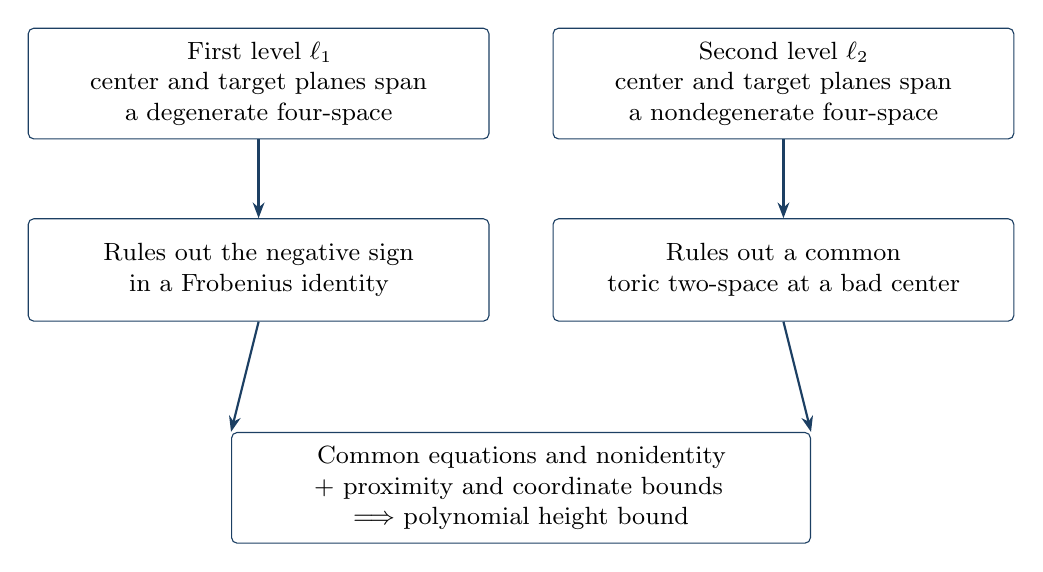
\begin{tikzpicture}[
  box/.style={draw=linkblue,rounded corners=2pt,align=center,
    text width=55mm,minimum height=13mm,inner sep=5pt,font=\small},
  arr/.style={-{Stealth[length=2mm]},draw=linkblue,thick},
  node distance=10mm and 8mm]
\node[box] (minus) {First level $\ell_1$\\
  center and target planes span\\a degenerate four-space};
\node[box,right=of minus] (plus) {Second level $\ell_2$\\
  center and target planes span\\a nondegenerate four-space};
\node[box,below=of minus] (sign) {Rules out the negative sign\\
  in a Frobenius identity};
\node[box,below=of plus] (torus) {Rules out a common\\
  toric two-space at a bad center};
\draw[arr] (minus)--(sign);
\draw[arr] (plus)--(torus);
\node[box,text width=70mm,below=14mm of $(sign.south)!0.5!(torus.south)$]
  (height) {Common equations and nonidentity\\
  + proximity and coordinate bounds\\
  $\Longrightarrow$ polynomial height bound};
\draw[arr] (sign.south)--(height.north west);
\draw[arr] (torus.south)--(height.north east);
\end{tikzpicture}
\caption{The two level incidences have different roles. The first is used
to exclude the negative sign in the nonidentity argument; the positive
sign is excluded by the Frobenius multiplier. The second excludes
proximity to centers with non-potentially-good reduction. The height
conclusion uses common equations at the retained places, nonidentity on
algebraic boundary branches, the large proximity sum, and the small
positive coordinate logarithms described in the text. The diagram is
schematic: all plane positions are in the separately marked finite-field
quadratic spaces.}
\label{fig:two-incidences}
\end{figure}


\subsection{Conventions and organization}

All heights are absolute logarithmic heights. Place sums use normalized
absolute-height weights, so extending a field preserves the sum for
pulled-back quantities. Constants may depend on the curve, the center,
fixed levels, frames and other fixed data. They never depend on the
varying target, its height or degree, or a varying residue characteristic.
In an estimate described as polynomial, the exponent is fixed.

We use covariant first homology and its de Rham and prime-to-residue-
characteristic \'etale realizations. The term \emph{ordinary point} for a
differential equation means a point where the connection has no
singularity; it places no ordinarity condition on the reduction of an
abelian variety. Every reduction of an endomorphism plane uses its
saturation in the specified integral lattice.

\Cref{int:section} states the interpolation theorem and explains its
proof mechanism.
\Cref{geo:section} constructs the geometric systems and controls the
exceptional Hecke correspondences. \Cref{inc:section} gives the two
incidences and excludes bad-center disks. \Cref{ht:section} proves the
coordinate estimates, and \Cref{loc:section} constructs the local
equations with their quantitative bounds. \Cref{nid:section} rules out
identities and obtains the height bound. Finally,
\Cref{fin:section} proves \Cref{intro:squares,intro:zp} and the
special-closure corollary. The complete proof of the interpolation
theorem is given in \Cref{int:proof}.

\section{Interpolation with a common small parameter}
\label{int:section}

The height theorem below applies to equations assembled from a fixed
collection of ordinary differential systems.  Its hypotheses distinguish
the global height of the target from the much smaller positive coordinate
logarithms at the places used for interpolation.  We state the theorem
and explain the graph construction that exploits this distinction here.
The full proof is given in Appendix~\ref{int:proof}.

\subsection{The quantitative statement}

For a tuple $x=(x_1,\ldots,x_r)$ over a number field $F$, write
\[
 h_{\mathrm{aff}}(x)
   =\sum_v w_v\log\max(1,|x_1|_v,\ldots,|x_r|_v),
 \qquad w_v=\frac{[F_v:\Q_v]}{[F:\Q]}.
\]
At an archimedean place we use the ordinary absolute value, so that a complex
place has weight $2/[F:\Q]$. At a finite place above $p$, the absolute
value extends $|p|_p=p^{-1}$. The same notation for a polynomial means the
height of its coefficient tuple.  A weighted subcollection of places may
split a place into its embeddings, with the corresponding weights.  When
$F$ is enlarged, these weights are split among the extensions of each
embedding.  In particular all sums for quantities defined over the old
field are unchanged.  We write $\sum_V w_v$ with this convention even when
the subcollection is described in terms of embeddings.

An \emph{ordinary germ} below is a horizontal analytic solution in a rational
frame in which the connection is regular at the specified center.  This is
a condition on a differential equation.  The rank, frame, center, and curve
carrying each such equation are fixed.

\begin{theorem}[Conditional height bound]\label{int:height}
Fix an ambient dimension $N$, a bound $s_0$ for the number of equations,
an integer $b$ bounding the degrees of the polynomial combinations below,
and a real constant $C_0\geq2$.  Fix also a finite list of algebraic regular
germs and ordinary horizontal matrix germs on fixed algebraic curves over
number fields.  Dual and inverse matrices are allowed in this list.
Then there is a constant $C$, depending only on these fixed data, with the
following property.

Let $d,h\geq2$ and let $z=(a,U)\in\mathbb A^N(\Qbar)$ with $a\ne0$.
Suppose a weighted subcollection $V$ and $1\leq s\leq s_0$ equations
\begin{equation}\label{int:equations}
 E_\alpha(a,U)=\sum_{j\geq0}a^j e_{\alpha,j}(U)=0
 \quad(1\leq\alpha\leq s)
\end{equation}
satisfy the following conditions.
\begin{enumerate}[label=\textup{(\roman*)}]
\item The point and the selected places satisfy
\begin{align}
 h_{\mathrm{aff}}(z)&\leq C_0d^{C_0}h,
 &|a|_v&<1\quad(v\in V),\label{int:global-input}\\
 \sum_{v\in V}w_v\log |a|_v^{-1}
   &\geq \frac{h}{C_0d^{C_0}},
 &\sum_{v\in V}w_v\log^+\|U\|_v
   &\leq C_0d^{C_0}(1+\log h)^{C_0}.
 \label{int:local-input}
\end{align}
Here $\|U\|_v$ is the maximum of the coordinate absolute values.
\item The coefficients are polynomials over a number field containing the
target and equation data, with
\begin{equation}\label{int:coefficient-input}
 \deg e_{\alpha,j}\leq C_0(1+j),\qquad
 h_{\mathrm{aff}}(e_{\alpha,j})
  \leq C_0(1+j+d)^{C_0}(1+\log h)^{C_0}.
\end{equation}
The same equations are used at every selected embedding.  They converge
there at the target, and there are numbers $b_v\geq0$ such that, for all
$\ell\geq0$ and all $\alpha$,
\begin{align}
 \left|\sum_{j\geq\ell}a^j e_{\alpha,j}(U)\right|_v
   &\leq |a|_v^\ell\exp((\ell+1)b_v),\label{int:tail-input}\\
 \sum_{v\in V}w_vb_v
   &\leq C_0d^{C_0}(1+\log h)^{C_0}.
\end{align}
\item As analytic functions in the variables $(a,U)$, the $E_\alpha$ are
polynomial combinations of degree at most $b$ of the coordinates and the
fixed germs evaluated at $a$, and possibly at $aR$, where $R$ is one of
the coordinates of $U$.  Their constant coefficients may depend on the
target.  The algebraic germs are regular functions on the specified local
curve charts.  Thus every expression is also a convergent complex analytic
germ near any finite point of $a=0$.
\item Let $W\subseteq\mathbb A^N_{\Qbar}$ be any irreducible closed
subvariety containing $z$ on which $a$ is nonconstant.  For each prime
divisor $D$ in its finite normalization lying above a component of
$W\cap\{a=0\}$, at least one $E_\alpha$ is not identically zero as an
analytic germ on the local branch at a general point of $D$.
\end{enumerate}
Then $h\leq Cd^C$.
\end{theorem}

The quantifier in condition \textup{(iv)} includes varieties defined using
the coefficients of the equations and the auxiliary polynomials constructed
below.  It concerns the germ on a whole local branch, rather than its value
on the boundary divisor.  No bound on the degree of the field of equation
coefficients is part of this theorem.

For the elliptic-square application, the inputs to conditions
\textup{(i)--(iii)} are assembled in \Cref{loc:groups}, and condition
\textup{(iv)} is verified in \Cref{nid:nonidentity}; the resulting height
bound is stated in \Cref{nid:height}.  We next explain why the theorem
requires nonidentity on every algebraic branch, and why small positive
local logarithms are needed in addition to a global height bound.

\subsection{Why the graph gives a height bound}

The proof constructs an auxiliary polynomial of degree $L$ whose value
at the target gains a factor $a^n$ at the selected places.  To make the
product formula useful, the construction must allow a sufficiently
large ratio $n/L$.
The graph construction makes this possible by lowering the dimension
of the boundary on which the interpolation conditions are imposed.

Start with $W=\mathbb A^N$.  During the proof, $W$ will be an irreducible
algebraic subvariety containing $z$, with controlled degree and defining
heights.  Write $k=\dim W$ and first suppose that $a$ varies on $W$ and
that $W\cap\{a=0\}$ is nonempty.  Condition \textup{(iv)} and an ordinary
differential multiplicity estimate give an integral linear combination
$E=\sum c_\alpha E_\alpha=\sum_{j\geq0}a^je_j(U)$ and an integer $m$
such that its truncation
\[
 F=E_{<m}:=\sum_{j=0}^{m-1}a^je_j(U)
 \quad\text{satisfies}\quad
 \ord_D F<m\ord_D a
\]
on every normalized boundary divisor $D$.  The coefficients $c_\alpha$
and $m$ are polynomially bounded in $\deg W$.  This strict inequality
means that $F/a^m$ has a pole at the generic point of every such divisor;
a nonzero restriction of $E$ to the boundary itself is not required.

Let $W'$ be the affine closure of the graph of $q=F/a^m$ over $a\ne0$.
It has dimension $k$.  Its boundary over $a=0$ has no point above a general
point of any boundary divisor of $W$, because $q$ has a pole there.
Thus the projection of $W'\cap\{a=0\}$ to $W$ has dimension at most
$k-2$.  Imposing $q=-e_m(U)$ fixes the graph coordinate, so
\[
 \dim\bigl(W'\cap\{a=0,\ q+e_m(U)=0\}\bigr)\leq k-2.
\]
For $k=1$ this intersection is empty.  This is a bound on the indicated
incidence, not on the whole graph boundary, whose fibers may have
positive dimension.

The lifted target $z'=(a,U,F(z)/a^m)$ has a different useful property.
At each selected place $E(z)=0$, and therefore
\[
 q(z')=-a^{-m}\sum_{j\geq m}a^je_j(U).
\]
The tail estimate bounds the positive local logarithm of this new
coordinate by $(m+1)b_v$, with the errors enlarged to accommodate the
chosen integral combination.  Hence $z'$ still has small positive
local logarithms, although its global height can be proportional to $h$.

Choose equations generating an ideal $I$ whose zero set is $W'$ and put
\[
 F_n=q+\sum_{j=0}^{n-1}a^je_{m+j}(U).
\]
The dimension bound above permits a polynomial $P$, nonzero on $W'$,
with
\[
 \deg P\leq L,\qquad P\in(I,a^n,F_n),\qquad n=cL,
\]
for any prescribed positive integer $c$, with $L$ polynomially bounded
in $c$ and the degree bounds of the construction.  Here membership is
in the displayed ideal itself, even if $I$ is nonradical.  The reason
for the freedom in $c$ is a count of linear conditions.  For $k\geq2$,
reducing successively through $n$ powers of $a$ imposes
$O(n(L+n)^{k-2})$ conditions, with a constant polynomial in the defining
degree bounds.  Restrictions of degree-$\leq L$ polynomials to $W'$
span a space of dimension at least $\binom{L+k}{k}$.  For $n=cL$ these
grow respectively as $L^{k-1}$ and $L^k$.  When $k=1$ there are no
conditions.  This saving of one power of $L$ is the purpose of the graph.

At the selected places, evaluating the ideal-membership certificate and
using the tail bound gives the factor $|a|_v^n$.  Even if the certificate
has degree larger than $L$, its degree multiplies only the small
positive local logarithms of $z'$.  At the remaining places one evaluates
$P$ itself, so the global height cost is proportional to $Lh$.
Consequently, if $P(z')\ne0$, the product formula gives an inequality
of the form
\[
 0\leq\left(-\frac n{A(d)}+L C(d)\right)h
        +D(d)(1+\log h)^B,
\]
where $A,C,D$ are fixed polynomials and $B$ is fixed.  The polynomials
$A,C$ are determined before $c$ is chosen.  Taking $c$ sufficiently
large, still polynomially bounded in $d$, makes the coefficient of $h$
negative and yields a polynomial bound for $h$ in $d$.

If that bound does not hold, $P(z')=0$.  Substituting $q=F/a^m$ and
clearing denominators gives a polynomial nonzero on $W$ and zero at
$z$.  An irreducible component through $z$ of its zero set in $W$
has smaller dimension and controlled degree and height.  This explains
the universal quantifier in condition \textup{(iv)}: the next variety
is chosen using the equations and the auxiliary polynomial.  After at
most $N$ such steps, either the height is bounded or one reaches a
variety disjoint from $a=0$.  If $G_1,\ldots,G_r$ define that variety,
a polynomial identity $1=aA+\sum_\rho G_\rho A_\rho$ and the small
positive local logarithms give the bound directly.
Appendix~\ref{int:proof} proves these degree, height, and multiplicity
assertions and the descent in detail.

\section{The geometric systems and a finite list of correspondences}
\label{geo:section}

We first fix the curves, the family, and an elliptic-square center.  The
trace-free self-adjoint endomorphisms form a five-dimensional orthogonal
system.  Its monodromy gives an alternative for two varying points: the
two systems have product monodromy, or their joint image lies in a
polarized isogeny correspondence.  The final result of this section
reduces the latter alternative to a fixed finite list.  This list is
chosen before the auxiliary levels of \Cref{inc:markings}.

\subsection{Fixed covers and the center}

\begin{proposition}\label{geo:setup}
In proving \Cref{intro:squares}, we may work with a smooth geometrically
irreducible curve $S$ over a fixed number field, a principally polarized
abelian scheme $\mathscr A\to S$, and a nonconstant finite map from $S$
onto a dense open of the original curve $C$.  We may equip the family
with full symplectic levels at two distinct fixed primes at least three.
Under the supposition that the required elliptic-square locus is
infinite, we may fix a point $t_0\in S(\Qbar)$ in that locus.

Further fixed finite covers, normalization, and removal of finite sets
preserve this reduction.  After enlarging a fixed field of definition
$K$, there is a constant $b$ such that every selected lift $t$ of a
retained coarse point $s$ satisfies
\begin{equation}\label{geo:degree-descent}
 [K(s):K]\leq [K(t):K]\leq b[K(s):K].
\end{equation}
The smooth projective completion of $S$ and the divisor $[t_0]$ are
available even when $C$ is complete.
\end{proposition}

\begin{proof}
Choose distinct primes $r_1,r_2\geq3$ and put $N=r_1r_2$.
These preliminary levels give a fine moduli cover.  The auxiliary
incidence primes will be chosen separately in \Cref{inc:markings},
after the correspondence list has been fixed.
After adjoining the requisite roots of unity, the fine Siegel moduli
space $\A_2(N)$ carries a universal principally polarized abelian
scheme and has a finite surjective forgetful map to the coarse space
$\A_2$; its analytic uniformization and the algebraicity of the
universal family are described in
\cite[Theorem~4.6 and Corollary~4.7]{MilneModuli2013}.
Take an irreducible component of its pullback to $C$ that
dominates $C$, and normalize.  Normalization is finite for a curve over
a field of characteristic zero.  The resulting curve is smooth, and
pullback supplies the abelian scheme.  Removing the preimages of any
finite exceptional set of coarse points leaves a finite surjective map
onto the complementary open of $C$.

All these varieties, components, morphisms, and level structures are
defined over a number field after a fixed enlargement.  The fibers of
a fixed finite map have bounded length; on a dense open this length is
its degree.  The residue field degree of any point in such a fiber is
at most that length.  This proves \eqref{geo:degree-descent}, with the
degrees of any additional fixed covers included in $b$.  It also shows
that the image of every omitted finite set is finite.  An infinite
coarse locus therefore has infinitely many lifts after every such
fixed omission, and we choose one of them as $t_0$.  Later covers may
be supplied with a fixed lift of this point; we then reuse $S,t_0$ for
the refined data.  Open charts and frames used at the center are
chosen to contain it.

A smooth curve over a number field has a smooth projective completion.
The point $t_0$ is an interior point of the moduli family, and its
divisor has positive degree on that completion.  This construction
uses no geometric boundary point and imposes no condition on the
arithmetic reduction of $\mathscr A_{t_0}$.
\end{proof}

Fix a number field $K_C$ defining the original coarse curve.  There
are only finitely many coarse conjugate curves
\begin{equation}\label{geo:coarse-curves}
 C_1,\ldots,C_e\subset\A_2,
\end{equation}
obtained by applying embeddings of $K_C$ into $\Qbar$.  All conjugate
families used below have coarse images in this list.  Enlarging the
field to define centers, levels, or individual endomorphisms does not
add coarse images: the image of $C$ depends only on the restriction
of the embedding to $K_C$.  We always retain the closed coarse curves
in \eqref{geo:coarse-curves}, even when their working parameter curves
have been restricted to open subsets.

\subsection{The five-dimensional orthogonal system}

Let $H=R_1\mathscr A_*\Q$ denote rational covariant first homology.
The polarization gives an alternating form $\psi$, with its usual
Tate twist in the different realizations.  For an operator $D$, write
$D^\dagger$ for the adjoint defined by
$\psi(Dv,w)=\psi(v,D^\dagger w)$.  Define
\begin{equation}\label{geo:operator-space}
 \cP=\{D\in\End(H):D^\dagger=D,\ \Tr_H(D)=0\},
 \qquad \langle D,E\rangle=\Tr_H(DE).
\end{equation}
These definitions commute with all the realization functors used
later.  On actual endomorphisms, $\dagger$ is the Rosati involution
of the given principal polarization.

\begin{proposition}\label{geo:five-space}
The system $\cP$ has rank five and a split nondegenerate trace pairing.
Conjugation induces a surjective morphism
\[
 \GSp_4\longrightarrow\SO(\cP)
\]
with scalar kernel.  Its restriction to $\Sp_4$ is the spin covering,
with kernel $\{1,-1\}$, and $\cP$ is absolutely irreducible.
For every odd prime $\ell$, the lattice
\begin{equation}\label{geo:integral-lattice}
 \Lambda_\ell=
 \{D\in\End_{\Z_\ell}(T_\ell\mathscr A_t):
       D^\dagger=D,\ \Tr(D)=0\}
\end{equation}
is free of rank five with unimodular trace pairing.

If $\mathscr A_t$ is isogenous to the square of a non-CM elliptic
curve, then
\begin{equation}\label{geo:hodge-plane}
 F_t=\End^0(\mathscr A_t)\cap\cP_t
\end{equation}
is a rational two-dimensional plane on which the trace pairing is
positive definite.  Here the intersection denotes Hodge
endomorphisms in the Betti realization, equivalently actual rational
endomorphisms in every realization.
\end{proposition}

\begin{proof}
Use a symplectic basis, with matrix
$J=\left(\begin{smallmatrix}0&I_2\\-I_2&0\end{smallmatrix}\right)$.
The equations $D^{\mathsf t}J=JD$ and $\Tr D=0$ give exactly
\begin{equation}\label{geo:matrix-model}
 D=\begin{pmatrix}A&uK_2\\vK_2&A^{\mathsf t}\end{pmatrix},
 \qquad
 A=\begin{pmatrix}a&b\\c&-a\end{pmatrix},
 \qquad K_2=\begin{pmatrix}0&1\\-1&0\end{pmatrix}.
\end{equation}
Multiplication gives
\begin{equation}\label{geo:trace-form}
 D^2=(a^2+bc-uv)I_4,
 \qquad \Tr(D^2)=4(a^2+bc-uv).
\end{equation}
Thus the form is the orthogonal sum of a nonzero one-dimensional
form and two hyperbolic planes.  Its Gram determinant in the five
coordinates displayed above is $64$, a unit over every $\Z_\ell$
with $\ell$ odd.  A principal polarization makes the Tate module
symplectically unimodular, so the same calculation proves
\eqref{geo:integral-lattice}.

Conjugation by a symplectic similitude preserves both conditions in
\eqref{geo:operator-space} and the trace pairing.  Since $\GSp_4$ is
connected, its orthogonal image has determinant one.  The induced
action of $\Sp_4$ is nontrivial, as is already seen by conjugating the
matrices in \eqref{geo:matrix-model}.  The simple Lie algebra
$\mathfrak{sp}_4$ consequently has zero kernel in this action.  Both
$\Sp_4$ and $\SO_5$ have dimension ten, so the image is all of
$\SO_5$.  The finite kernel is central in the connected group
$\Sp_4$ and is exactly $\{1,-1\}$.  Over an algebraic closure a
similitude is a scalar times a symplectic element, which proves the
scalar-kernel assertion for $\GSp_4$ and identifies the restriction
as the spin covering.  The natural representation of $\SO_5$ is
irreducible over an algebraically closed field of characteristic
zero: the orbit of any nonzero vector, whether isotropic or not,
spans the entire quadratic space.  This proves absolute
irreducibility.  Equivalently, $D\mapsto\psi(D\cdot,\cdot)$
identifies the self-adjoint space with alternating two-forms, and
the trace-free summand with the primitive exterior-square
representation.

For the last assertion, put $A=\mathscr A_t$.  The equivalence between
complex abelian varieties up to isogeny and polarizable rational
Hodge structures of type $(-1,0),(0,-1)$ identifies
$\End^0(A)$ with the Hodge endomorphisms of $H_1(A,\Q)$
\cite[Theorem~4.1]{MilneShimura1995}.  Write
$H_1(A,\Q)=H_1(E,\Q)\otimes\Q^2$ using the given unpolarized
isogeny.  Since $E$ has no CM, its endomorphism algebra is $\Q$;
the Hodge endomorphism algebra of $A$ is therefore $\Mat_2(\Q)$.
An alternating polarization on this tensor product has the form
$\psi_E\otimes B$, where $B$ is a symmetric rational form on
$\Q^2$.  Indeed, each of its four matrix entries is a Hodge
alternating pairing on $H_1(E,\Q)$, hence a scalar multiple of
$\psi_E$; alternation of the total form makes these four scalars
symmetric.  Positivity of the polarization, after choosing the sign
of $\psi_E$, makes $B$ positive definite.  The Rosati involution on
$\Mat_2(\Q)$ is consequently the adjoint for $B$.

Its self-adjoint part has dimension three and contains the identity.
The homology trace on this algebra is twice the ordinary matrix
trace, so imposing trace zero leaves dimension two.  Over $\R$,
conjugation by the positive square root of $B$ turns a self-adjoint
matrix $D$ into a symmetric matrix $D_0$.  Hence, for $D\ne0$,
\[
 \Tr_{H_1(A)}(D^2)=2\tr(D_0^2)>0.
\]
This proves the asserted positivity for every principal
polarization, without requiring the initial isogeny from $E^2$ to
preserve it.
\end{proof}

Fix a labeled pair $\mathbf B=(B_1,B_2)$ of linearly independent
integral endomorphisms spanning $F_0:=F_{t_0}$; clear denominators
in a rational basis to obtain it.  At any target and prime, the
plane lattice used for reduction is
\begin{equation}\label{geo:saturated-plane}
 \Pi_{t,\ell}=(F_t\otimes\Q_\ell)\cap\Lambda_\ell.
\end{equation}
It is saturated and has rank two, so its image in
$\Lambda_\ell/\ell\Lambda_\ell$ has dimension two.  We do not
identify this image with the span of a chosen pair reduced modulo
$\ell$: that pair can fail to be a lattice basis.  At the fixed
center, the restriction of the pairing to
$\Pi_{t_0,\ell}$ is nondegenerate modulo $\ell$ outside finitely
many primes.  To see finiteness, intersect $F_0$ with the integral
Betti operator lattice, choose a $\Z$-basis of this intersection,
and exclude the prime divisors of its nonzero Gram determinant.
Betti--Tate comparison gives precisely the lattices above.

\subsection{Full and joint monodromy}

\begin{proposition}\label{geo:monodromy}
The connected algebraic monodromy of $H$ is $\Sp_4$, and that of
$\cP$ is $\SO_5$.  This remains true on every fixed finite cover,
on a dense open, and for the conjugate families under consideration.
The same connected monodromy is obtained by pullback to a smooth
connected algebraic variety mapping dominantly to the base curve.

Suppose a smooth connected algebraic variety $W$ maps dominantly to
two such curves.  The connected joint monodromy on the two
five-dimensional systems is either $\SO_5\times\SO_5$, or the
coarse joint image of $W$ is contained in a polarized isogeny
correspondence.  If only the first projection varies, its connected
monodromy is still $\SO_5$.
\end{proposition}

\begin{proof}
Hodge genericity in Siegel moduli means that the generic
Mumford--Tate group of $H$ is $\GSp_4$.  The variation is pure and
polarizable and comes from an abelian scheme over a smooth
algebraic curve.  Thus it is among the good variations to which
the connected-monodromy normality theorem applies: connected
algebraic monodromy is a normal subgroup of the derived generic
Mumford--Tate group
\cite[\S5, Theorem~1]{Andre1992}.  Since $\Sp_4$ is almost simple,
the connected monodromy is trivial or all of $\Sp_4$.

Here is a direct exclusion of the trivial possibility.  It would
make the monodromy group finite, and a finite cover would trivialize
the integral local system.  The period map would then be a
single-valued holomorphic map from a smooth algebraic curve to
Siegel space.  Realize Siegel space as a bounded domain in
$\C^3$.  Each coordinate of this map is bounded near each of the
finitely many missing points of the smooth projective completion,
so has a removable singularity there.  Every extended coordinate
is constant on the projective curve.  The family would have
constant moduli image, contrary to its domination of $C$.
This also explains concretely the applicability of
\cite[\S6, Remark~1]{Andre1992}.  The monodromy conclusion is
independent of the Mumford--Tate group at the chosen center.
\Cref{geo:five-space} now gives the assertion on $\cP$.

A nonconstant morphism between smooth algebraic curves restricts,
after removal of finitely many points, to a finite etale morphism
onto a dense open.  Its topological fundamental group therefore
has image of finite index in that of this open; the latter maps
surjectively to the fundamental group of the original curve.
Finite-index subgroups have the same connected Zariski closure.
This proves invariance under finite covers and open restrictions.
For a dominant map from a higher-dimensional smooth variety,
choose an algebraic curve in that variety whose projection is
nonconstant, and normalize it.  Such a curve is obtained by
successive general affine hyperplane sections through a point
where the differential of the projection is nonzero.  Its
monodromy is contained in the pullback monodromy and is already
full by the curve case.  This proves the pullback assertion.

For completeness, full monodromy persists under field conjugation
without a choice of a conjugation-compatible complex period map.
Choose a prime $\ell$.  The Betti monodromy is Zariski dense in
$\Sp_4$, so its image on $H\otimes\Q_\ell$ is Zariski dense in
$\Sp_{4,\Q_\ell}$.  The comparison of topological and geometric
etale fundamental groups identifies the latter image with a dense
subgroup of the geometric etale monodromy image.  A field
conjugation identifies the corresponding geometric etale families
and their symplectic Tate systems.  Applying the same comparison
on the conjugate complex curve proves that its Betti algebraic
monodromy is again full.  In particular its coarse image is Hodge
generic: otherwise its monodromy would lie in the derived group
of a proper generic Mumford--Tate subgroup.  One can also use
the preservation of Siegel special subvarieties by conjugation.

It remains to prove the assertion concerning $W$.  Work at a
generic Mumford--Tate point of the direct sum of the two pulled
back homology variations, in rational symplectic bases.  Both
projections of its connected algebraic monodromy are full, by the
pullback assertion just proved.  Pass to the adjoint groups
$G_1,G_2$, each isomorphic to $\operatorname{PGSp}_4$ and to the
corresponding $\SO_5$.  Let $M\subset G_1\times G_2$ be the
connected joint image.  The kernel of either projection is a
normal subgroup of the other adjoint simple group.  Thus either
one kernel is the whole factor, giving $M=G_1\times G_2$, or both
are trivial and
\begin{equation}\label{geo:graph-group}
 M=\{(x,\phi(x)):x\in G_1\}
\end{equation}
for a $\Q$-isomorphism $\phi:G_1\to G_2$.  This is the group
form of Goursat's argument; no passage to a merely real graph has
been made.

The remaining task is to lift this adjoint graph to a positive rational
similitude identifying the homology Hodge structures.  This requires
both the graph relation and the polarization characters.
Let $T$ be the generic Mumford--Tate group of the direct sum.
The normality theorem applies on the smooth algebraic variety
$W$ and says that $T$ normalizes connected monodromy.  Its
adjoint image therefore normalizes \eqref{geo:graph-group}.
The normalizer of this graph in $G_1\times G_2$ is the graph
itself.  Indeed, normalization by $(u,v)$ says that
$v\phi(x)v^{-1}=\phi(u)\phi(x)\phi(u)^{-1}$ for all $x$;
the trivial center of $G_2$ gives $v=\phi(u)$.

The root diagram of type $C_2$ has no nontrivial automorphism,
so every automorphism of its adjoint split group is inner.
The conjugating element is unique, hence is rational when the
automorphism is rational.  Finally the sequence
\[
 1\longrightarrow\Gm\longrightarrow\GSp_4
   \longrightarrow\operatorname{PGSp}_4\longrightarrow1
\]
and $H^1(\Q,\Gm)=1$ lift it to a rational similitude
$g\in\GSp_4(\Q)$.  Consequently the two Hodge homomorphisms,
after conjugation by $g$, agree in the adjoint group.  Their
remaining difference is a scalar character $c$ of the Deligne
torus.  Each polarization is a morphism of Hodge structures
$\psi_i:H_i\otimes H_i\to\Q(1)$.  Thus the full similitude
character $\nu\circ h_i$ is the character of the same Tate
structure $\Q(1)$ for both $i$, on the whole Deligne torus.
Since a scalar $c$ has multiplier $c^2$, the equality
$h_2=c\,g h_1g^{-1}$ therefore gives $c^2=1$.
The Deligne torus is connected as an
algebraic group, whence $c=1$.  We have obtained a rational Hodge
isomorphism on $H_1$, not just an identification of its adjoint
representation.

Its multiplier is positive.  For if $J_i$ are the complex
structures at this point, then $gJ_1=J_2g$, and positivity of
the two polarization metrics in
\[
 \psi_2(gv,J_2gv)=\nu(g)\psi_1(v,J_1v)
\]
forces $\nu(g)>0$.  By the rational Hodge equivalence
\cite[Theorem~4.1]{MilneShimura1995}, an integral multiple of
$g$ is a polarized isogeny.

This same $g$ describes an analytic open of the joint image.
Indeed, trivialize the rational local system in a simply
connected open.  For each of its countably many rational tensors,
the locus where it is Hodge is closed analytic.  A point outside
the union of those loci that are proper has the generic
Mumford--Tate group.  Every tensor Hodge at that point is
therefore Hodge throughout the open.  By the tensor-stabilizer
description of the Mumford--Tate group, all Hodge homomorphisms
there factor through the transported generic group $T$.
Applying the graph relation
for that group makes $g$ a Hodge isomorphism throughout the
open.  The joint period map is therefore locally in the graph
of $g$, and its coarse image lies locally in the Hecke
correspondence $T_g$.  This correspondence is closed and
algebraic: it is the image of the finite polarized-isogeny
moduli correspondence, or equivalently of the quotient for
$\Gamma\cap g^{-1}\Gamma g$, where
$\Gamma=\Sp_4(\Z)/\{1,-1\}$.  An algebraic equation for $T_g$
vanishing on a nonempty analytic open of the irreducible image
vanishes on that image.  Thus the entire joint image lies in
$T_g$.  The claim when the second projection is constant follows
already from full monodromy of the first projection.
\end{proof}

\subsection{Finitely many dominating correspondence types}

For $g\in\GSp_4(\Q)$ of positive multiplier, write $T_g$ for its
coarse Hecke correspondence in $\A_2\times\A_2$.  Scalar multiples
and integral changes of symplectic markings on either side give
the same correspondence.  A \emph{dominating relation} between
closed curves $C_i,C_j$ means an irreducible algebraic curve
contained in $(C_i\times C_j)\cap T_g$ with both projections
dominant.

\begin{proposition}\label{geo:hecke-list}
For the fixed finite collection \eqref{geo:coarse-curves}, only
finitely many coarse Hecke correspondences admit a dominating
relation between a pair of these curves.  In particular there is
a fixed finite list $\mathcal T$ containing every exceptional
joint image in \Cref{geo:monodromy}.  We may take this list closed
under exchanging the two factors and choose, for every member,
positive integral multipliers for isogenies realizing all its
pairs.  The list and these multipliers are fixed before any
additional auxiliary levels are chosen.
\end{proposition}

\begin{proof}
We prove finiteness, including the analytic stabilizer assertion
on which it depends.  Use one fixed torsion-free principal level $N$ as
in \Cref{geo:setup}.  There are finitely many irreducible closed
curves $D_\alpha\subset\A_2(N)$ lying above the curves $C_i$.
All of them have full connected monodromy by
\Cref{geo:monodromy}.  Write $\mathfrak H_2$ for Siegel space and
\[
 G=\GSp_4(\R)^+/\R^\times
     \simeq\Sp_4(\R)/\{1,-1\},
 \qquad \Gamma_N\subset G
\]
for the effective level group.  The map
$\pi_N:\mathfrak H_2\to\A_2(N)(\C)$ is a covering: the choice
of torsion-free level eliminates stabilizers.

\paragraph{Lift components and their integral stabilizers.}
Remove the finitely many singular points of $D_\alpha$, and
choose a connected component $U_\alpha$ of its inverse image.
Let $Y_\alpha$ be its closure in $\mathfrak H_2$.  It is a
closed irreducible analytic curve.  To check this last assertion,
the inverse image of $D_\alpha$ is locally analytically identical
to $D_\alpha$ under the covering.  It has a locally finite
collection of curve branches, and closure of a chosen connected
smooth part joins precisely its continued branches.  The
normalization of that closure is connected, so the closure is
irreducible.  Conversely every irreducible component arises this
way.  The deck group acts transitively on these components, by
path lifting along the connected nonsingular part of
$D_\alpha$.

Put $\Delta_\alpha=\Gamma_N\cap\Stab_G(Y_\alpha)$.  This is
also the subgroup preserving $U_\alpha$, and covering-space
monodromy identifies it with the image of
$\pi_1(D_\alpha^{\mathrm{reg}})$ in $\Gamma_N$.  In particular
it is Zariski dense in $G$.  Moreover
\begin{equation}\label{geo:lift-quotient}
 \Delta_\alpha\backslash U_\alpha
       \simeq D_\alpha^{\mathrm{reg}}.
\end{equation}
The identification follows because any two lifts of a point in
the chosen component differ by a deck transformation preserving
that component.  Removing additional finite sets, if needed,
has no effect on these statements.

\paragraph{Closedness and discreteness of the real stabilizer.}
Let $L_\alpha=\Stab_G(Y_\alpha)$.  If $g_n\in L_\alpha$ and
$g_n\to g$ in $G$, closedness of $Y_\alpha$ gives
$gY_\alpha\subset Y_\alpha$.  Applying the same argument to
$g_n^{-1}$ proves the reverse inclusion.  Thus $L_\alpha$ is a
closed subgroup of the real Lie group $G$.

Its Lie algebra is invariant under $\Ad(\Delta_\alpha)$.
The stabilizer of a linear subspace of $\mathfrak{sp}_4(\R)$
under the adjoint action is algebraic.  Zariski density therefore
makes $\Lie(L_\alpha)$ invariant under all of $G$, hence an
ideal in the simple real Lie algebra $\mathfrak{sp}_4(\R)$.
It is zero or the entire Lie algebra.  The second possibility
would imply $L_\alpha=G$, since $G$ is connected, and would make
the nonempty curve $Y_\alpha$ invariant under the transitive
action of $G$ on the three-dimensional domain $\mathfrak H_2$.
This is impossible.  Thus $\Lie(L_\alpha)=0$ and $L_\alpha$
is discrete.

\paragraph{Finite area of the integral quotient.}
Equip $\mathfrak H_2$ with its invariant Hermitian metric, and
use the induced area on the regular part of $Y_\alpha$.  We
claim
\begin{equation}\label{geo:finite-area}
 \operatorname{area}(\Delta_\alpha\backslash
                         Y_\alpha^{\mathrm{reg}})<\infty.
\end{equation}
By \eqref{geo:lift-quotient}, it suffices to estimate the induced
metric on the normalization of $D_\alpha$.  Its smooth
projective completion adds finitely many punctures.

Here is the required uniform disk estimate.  Move the value at
zero of a holomorphic disk map into $\mathfrak H_2$ to $iI_2$
by an element of $G$, and use the Cayley transform to the
bounded domain of symmetric two-by-two matrices of operator
norm less than one.  The resulting map $Z$ has $Z(0)=0$.
Scalar Schwarz applied to $u^*Z v$ for unit vectors $u,v$ gives
$\|Z'(0)\|_{\mathrm{op}}\leq1$.  At the origin the invariant
metric is a fixed positive multiple of
$\tr(dZ\,dZ^*)$.  Hence the derivative has a uniform bound.
Precomposing with disk automorphisms gives, with an absolute
constant $c$, the metric inequality
\[
 f^*ds^2_{\mathfrak H_2}
       \leq c\frac{|dz|^2}{(1-|z|^2)^2}
\]
for every holomorphic disk map $f$.

On a punctured disk $0<|q|<R$ in the normalization, lift its
universal covering disk to $\mathfrak H_2$ and apply this
inequality.  It descends to
\begin{equation}\label{geo:cusp-area}
 ds^2\leq c'\frac{|dq|^2}
 {|q|^2\log^2(R/|q|)}.
\end{equation}
Its area integral for $0<|q|<r<R$ is bounded by a constant
times
\[
 \int_0^r\frac{d\rho}{\rho\log^2(R/\rho)}
       =\frac{1}{\log(R/r)}<\infty.
\]
The compact remainder has finite area by smoothness.  Zeros of
the derivative only decrease the area, and singular points and
their discrete lifts have area zero.  This proves
\eqref{geo:finite-area}.

\paragraph{Finite index in the full stabilizer.}
The action of $G$ on $\mathfrak H_2$ is proper: this symmetric
space is $G/K$ with $K$ compact.  Its restriction to the closed
discrete subgroup $L_\alpha$ is consequently proper, with finite
point stabilizers.  Choose a smooth point $y\in Y_\alpha$ and
write $F=(L_\alpha)_y$, a finite group.  Properness provides a
sufficiently small neighborhood $U$ of $y$ in the regular curve
of positive area $a$, such that $hU\cap U=\varnothing$ unless
$h\in F$.

For representatives $h_i$ of distinct double cosets in
$\Delta_\alpha\backslash L_\alpha/F$, the images of $h_iU$
in $\Delta_\alpha\backslash Y_\alpha$ are disjoint.  Indeed,
an intersection would imply
$h_i^{-1}\delta h_jU\cap U\ne\varnothing$ for some
$\delta\in\Delta_\alpha$, hence
$h_i^{-1}\delta h_j\in F$.  Each image has area at least
$a/|F|$, since only members of a conjugate of $F$ can identify
points within it.  Infinitely many such double cosets would
contradict \eqref{geo:finite-area}.  There are therefore finitely
many of them; because $F$ is finite, this proves
\begin{equation}\label{geo:finite-index}
 [L_\alpha:\Delta_\alpha]<\infty.
\end{equation}

\paragraph{Transporters and Hecke double classes.}
For two fixed lift components, consider the real transporter
\[
 \mathcal R_{\alpha\beta}
  =\{g\in G:gY_\alpha=Y_\beta\}.
\]
If it is nonempty and $g_0$ belongs to it, then
$\mathcal R_{\alpha\beta}=g_0L_\alpha$.
By \eqref{geo:finite-index} this set has finitely many right
$\Delta_\alpha$-cosets.  Among the cosets that meet the image
of $\GSp_4(\Q)^+$ choose rational representatives.  These give
finitely many integral double classes for all rational elements
of the transporter, because $\Delta_\alpha\subset\Gamma_N$
and passage to the full integral group only identifies more
classes.

Now suppose $T_g$ admits a dominating relation between two
coarse curves.  Over a smooth point of that relation, both
projections have nonconstant local parametrizations.  Lift them
to the fixed torsion-free level and then locally to Siegel space.  A
local sheet of the Hecke correspondence identifies the two
lifted arcs by a rational positive similitude in the integral
double class of $g$.  The arcs lie on some translates of
$Y_\alpha,Y_\beta$; applying deck transformations makes these
the chosen components.  The translated similitude takes a
nonempty open arc of $Y_\alpha$ into $Y_\beta$.  Its image of
$Y_\alpha$ and $Y_\beta$ are closed irreducible analytic curves
with a one-dimensional intersection, so the analytic identity
principle makes them equal.  The similitude thus belongs to the
transporter just considered.  There are finitely many pairs
$(\alpha,\beta)$ and finitely many double classes for each.
This proves the claimed finiteness of coarse correspondences.

Finally choose a rational similitude representative $g$ of each
retained class.  Multiplying it by a positive integer clears its
matrix denominators.  Its multiplier $m$ is then a positive
integer: applying the equality of alternating forms to a pair
of integral vectors of pairing one shows that the multiplier
is integral.  It yields an isogeny $f$ with
$f^*\lambda'=m\lambda$ at every pair of its correspondence.
This also follows from the finite moduli description by kernels
of such isogenies in the $m$-torsion.  Repeat the choice for the
inverse representatives to include both directions.  There are
only finitely many resulting positive integers.  The construction
has involved only the fixed coarse curves and an initial torsion-free
level; further levels change their parametrizations, not these
curves or the list.  Thus all multipliers are fixed before the
auxiliary incidence primes are selected.
\end{proof}

The finiteness just proved concerns dominating relations.  It places
no bound on the isogeny degrees of isolated pairs of points on the
two curves.  A pair on a retained correspondence, whether or not it
lies on a dominating component, does have an isogeny of that
correspondence's fixed multiplier.  Also, if an irreducible
algebraic joint image is contained in a retained correspondence on
a dense open, its whole image, including any specified target
pair where the maps are defined, is contained there by closedness.
These are precisely the two uses of the finite list in
\Cref{loc:equations,nid:nonidentity}.

\section{Two auxiliary markings and exclusion of bad disks}\label{inc:section}

We impose two conditions on the relative positions of the center and target
endomorphism planes.  The first will be used with Frobenius in
\Cref{nid:frobenius}.  The second rules out proximity to the center at
every place where it is not potentially good.  Both conditions concern
reductions of saturated planes; they impose no primitivity condition on
the particular endomorphisms later chosen to span those planes.

\subsection{Finite-field positions of two planes}

We first give the linear algebra uniformly in the target plane.  Write
$V$ for the split quadratic five-space obtained from a symplectic
four-space by the representation in \Cref{geo:five-space}.  We use the
associated symmetric bilinear form, and call the rank of its restriction
to a subspace the rank of that subspace.
The target is reduced from a saturated rank-two lattice, so it remains
a plane, but its restricted form may have rank zero, one, or two.
The lemma therefore allows an arbitrary target plane $H$.

\begin{lemma}\label{inc:finite-fields}
There is an absolute constant $q_0$ with the following property.  Let
$k$ be a finite field of odd cardinality $q>q_0$, let $H_0\subset V_k$
be a nondegenerate plane, and let $H\subset V_k$ be any plane.  There
are $g_-,g_+\in\Sp_4(k)$ such that
\[
 \dim(H_0+g_-H)=\dim(H_0+g_+H)=4,
\]
the first sum is degenerate, and the second is nondegenerate.
Here the action is the quadratic representation, so the assertion
does not require surjectivity of $\Sp_4(k)\longrightarrow\SO(V_k)$.
\end{lemma}

\begin{proof}
We will use the following elementary observation about rational charts.
The big Bruhat cell of the split group $\Sp_4$ has coordinates
$\mathbb A^4\times\Gm^2\times\mathbb A^4$: multiply the four negative
root subgroups, a diagonal torus element, and the four positive root
subgroups, in a fixed order.  Their matrices, their inverses, and their
actions on $V$ have Laurent-polynomial entries of bounded degrees in
these ten coordinates, independently of $k$.  The same assertion holds
for a big cell of a split parabolic, using its Levi root subgroups and
unipotent radical.  Conjugating a parabolic or inserting a fixed group
element changes coefficients and does not change these degree bounds.

Consequently, an open condition expressed by minors of a bounded-size
matrix in this representation can be tested on either chart by a
polynomial of degree at most an absolute constant $D$.  If the condition
holds at some geometric point, it holds on the corresponding dense
chart: both the group and the parabolic are geometrically irreducible.
Choose a minor that is not identically zero, clear its torus
denominators, and multiply by the torus coordinates.  The resulting
nonzero polynomial has a degree bounded by another absolute constant.
A nonzero polynomial of total degree less than $q$ cannot vanish on
all of $k^n$.  This follows by induction on $n$, applying the univariate
root bound to its nonzero coefficients.  Thus every such geometrically
nonempty open condition has a $k$-point once $q>q_0$, for one constant
$q_0$ that works for all planes under consideration.  No coefficient
height or isometry type enters this bound.

For the nondegenerate sum, work first over $\bar k$.  Choose a
nondegenerate four-space $M$ containing $H_0$, and write
$M=H_0\perp K$ with $\dim K=2$.  Choose bases in which both forms
are $I_2$.  The plane that is the graph of
$A=\diag(a,b):K\longrightarrow H_0$ is disjoint from $H_0$ and has
Gram matrix
\[
 I_2+A^{\mathsf t}A=\diag(1+a^2,1+b^2).
\]
Choices of $a,b\in\bar k$ give each of the ranks $0,1,2$.  Over
$\bar k$, bilinear forms on a two-space are classified by rank, so
there is a graph isometric to $H$, including when $H$ is degenerate.
Witt's extension theorem for subspaces of a nondegenerate space extends
this isometry to an orthogonal transformation of $V_{\bar k}$.
Its determinant can be changed by a reflection in a nonisotropic vector
perpendicular to the graph.  Such a vector exists: that perpendicular
has dimension three, whereas the largest totally isotropic subspace of
$V_{\bar k}$ has dimension two.  We obtain an element of $\SO(V_{\bar
k})$, which lifts to $\Sp_4(\bar k)$ by the spin covering.
Nonvanishing of the Gram determinant of the four concatenated basis
vectors is an open condition and implies their independence.  The
chart argument just proved supplies $g_+\in\Sp_4(k)$ uniformly.

For the degenerate sum, choose an isotropic line $L\subset H_0^\perp$
over $k$.  The perpendicular is a nondegenerate ternary space.  Every
such space over a finite field of odd cardinality is isotropic: after
diagonalization, the two sets
$\{ax^2:x\in k\}$ and $\{-c-by^2:y\in k\}$ each have
$(q+1)/2$ elements and therefore meet, giving an isotropic vector with
third coordinate $1$.  The three-space $H^\perp$ also has an isotropic
line over $k$.  If it is nondegenerate the same argument applies; if
it is degenerate its nonzero radical supplies one.

The group $\Sp_4(k)$ is transitive on the isotropic lines of $V_k$.
Indeed, under the primitive exterior-square realization these lines are
the Pl\"ucker lines of the Lagrangian two-spaces in the symplectic
four-space; symplectic bases show transitivity over $k$ itself.
Move the chosen line in $H^\perp$ to $L$.  After this preliminary
move, $H\subset L^\perp$.  Let $P$ be the stabilizer of $L$ in
$\Sp_4$ and put
\[
 Q=L^\perp/L.
\]
This is a nondegenerate ternary space.  The projection of $H_0$ is
a plane $\overline H_0\subset Q$ because $H_0\cap L=0$.
Over $\bar k$, the Levi action of $P$ on $Q$ includes $\SO(Q)$.
If $H$ contains $L$, its projection is a line.  This line can be
moved outside $\overline H_0$, since the standard representation of
$\SO(Q)$ is irreducible.  Its inverse image then meets $H_0$ trivially.

If $H$ does not contain $L$, its projection is a plane
$\overline H\subset Q$.  Move it so that
$\overline H\ne\overline H_0$.  Such a move exists since a plane
cannot be invariant under the irreducible group $\SO(Q)$.  The two
projected planes now meet in a line $J$.  The unipotent radical permits
an arbitrary change of the lift $Q\longrightarrow L^\perp$ by a
linear map $Q\longrightarrow L$.  Explicitly, choose a hyperbolic
pair $e,f$, with $L=\bar k e$ and $\langle e,f\rangle=1$, and
identify $Q$ with $(\bar k e+\bar k f)^\perp$.  For $z\in Q$ the
orthogonal unipotent transformation is
\[
 e\longmapsto e,\qquad
 n\longmapsto n-\langle n,z\rangle e,\qquad
 f\longmapsto f+z-\tfrac12\langle z,z\rangle e.
\]
These transformations lift to the unipotent radical in $\Sp_4$;
equivalently, in its symplectic realization that radical consists of
the matrices $\left(\begin{smallmatrix}I&Z\\0&I\end{smallmatrix}\right)$
with $Z$ symmetric.  Since the form on $Q$ is nondegenerate,
$n\mapsto-\langle n,z\rangle$ runs through all linear forms on
$Q$.  Choose it so that the lifts of the nonzero vectors of $J$ in
the moved $H$ and in the fixed $H_0$ are distinct.  Then
$H\cap H_0=0$.

We have exhibited a geometric point of $P$ where a four-by-four
minor of the concatenated bases of $H_0$ and the moved $H$ is
nonzero.  The parabolic chart argument gives such a point over $k$
for the same uniform lower bound on $q$.  Their sum, contained in
$L^\perp$ and of dimension four, is exactly $L^\perp$.  Its radical
is $L$, so it is degenerate.  This proves the first assertion and
completes all three possible target-rank cases.
\end{proof}

\subsection{Independent markings on one connected cover}

For a non-CM elliptic-square point $u$, denote its rational Hodge
endomorphism plane by $F_u$.  At an odd prime $\ell$, let
$\Lambda_{u,\ell}$ be the lattice of trace-free self-adjoint operators
on $T_\ell A_u$ from \Cref{geo:five-space}, and set
\begin{equation}\label{inc:saturation}
 \Pi_{u,\ell}=(F_u\otimes\Q_\ell)\cap\Lambda_{u,\ell},
 \qquad
 \overline\Pi_{u,\ell}=\Pi_{u,\ell}/\ell\Pi_{u,\ell}
       \ \subset\Lambda_{u,\ell}/\ell\Lambda_{u,\ell}.
\end{equation}
The quotient $\Lambda_{u,\ell}/\Pi_{u,\ell}$ is torsion free,
so the displayed reduction is an embedded two-space.  A full
symplectic $\ell$-marking identifies its ambient five-space with the
fixed $V_{\mathbb F_\ell}$.  This definition is independent of the
integral pair used to span $F_u$ rationally.

\begin{proposition}\label{inc:markings}
After one fixed finite cover of the curve in \Cref{geo:setup}, there
are distinct fixed odd primes $\ell_1,\ell_2$ and a fixed lift of the
center $t_0$ with the following properties.  Every non-CM elliptic-square
target on the previous curve has a lift $t$ for which, in the respective marked
five-spaces,
\begin{align}
 \overline\Pi_{t_0,\ell_1}+\overline\Pi_{t,\ell_1}
   &\text{ is a degenerate four-space},\label{inc:first}\\
 \overline\Pi_{t_0,\ell_2}+\overline\Pi_{t,\ell_2}
   &\text{ is a nondegenerate four-space}.\label{inc:second}
\end{align}
The prime $\ell_1$ divides none of the fixed Hecke multipliers in
\Cref{geo:hecke-list}.  The prime $\ell_2$ is different from every
residue characteristic at which the fixed center is not potentially
good.  Both center-plane reductions are nondegenerate.  The conditions
remain valid upon simultaneous conjugation of all the data, and the
degree of any chosen lift increases by at most a fixed factor.
\end{proposition}

\begin{proof}
Choose a symplectic integral Betti lattice.  Its geometric monodromy
group $\Gamma\subset\Sp_4(\Z)$ is finitely generated, because the
fundamental group of a smooth algebraic curve is finitely generated,
and is Zariski dense by \Cref{geo:monodromy}.  Strong approximation
for a finitely generated Zariski-dense subgroup of a connected,
simply connected, absolutely almost simple rational group gives
\[
 \Gamma\longrightarrow\Sp_4(\mathbb F_\ell)
 \quad\hbox{surjective for every sufficiently large prime }\ell;
\]
these are precisely the hypotheses of
\cite[Introduction, Theorem, p.~515]{MVW1984} for $\Sp_4$.

Fix $\ell_1>q_0$ outside this theorem's finite exceptional set,
the finitely many primes of degeneracy of the fixed center plane,
and the primes dividing the already fixed multipliers in
\Cref{geo:hecke-list}.  Its reduction kernel
$\Gamma_1$ has finite index in $\Gamma$.  Schreier's theorem gives
finite generation of $\Gamma_1$; its Zariski closure is still
$\Sp_4$, since a connected algebraic group cannot be a finite union
of translates of a proper closed subgroup.  Apply strong approximation
to $\Gamma_1$, and choose $\ell_2>q_0$ distinct from $\ell_1$,
outside its exceptional set, outside the center-plane degeneracy set,
and outside the residue characteristics of all non-potentially-good
places of $A_{t_0}$.  The last set is finite because the fixed abelian
variety has good reduction away from finitely many places.  All these
exclusions use fixed data.

It follows that
\begin{equation}\label{inc:product-reduction}
 \Gamma\longrightarrow
 \Sp_4(\mathbb F_{\ell_1})\times\Sp_4(\mathbb F_{\ell_2})
 \quad\hbox{is surjective}.
\end{equation}
To check this explicitly, first realize a prescribed element in the
first factor by an element of $\Gamma$; correct its second factor
using an element of $\Gamma_1$.  The cover parametrizing the two
full markings with fixed Weil pairings is therefore connected:
its monodromy acts transitively on the product torsor of markings.
After a fixed extension of the field of definition, it is a fixed
geometrically connected finite \'etale cover of our curve, carrying
both markings.  Fix any lift of $t_0$ to it.

For each target, \Cref{inc:finite-fields} prescribes a marking at
$\ell_1$ and, independently, a marking at $\ell_2$ satisfying
\eqref{inc:first} and \eqref{inc:second}.  The full product torsor
lies in the connected cover, so these choices give a point of that
cover.  We continue to write $S,t_0,t$ for the resulting curve,
center, and selected target.  Selection need not be an algebraic rule:
every point in a fiber of a finite morphism of fixed degree has degree
over the original point bounded by that degree.  Subsequent finite
omissions on the curve omit only finitely many points downstairs, as
in \Cref{geo:setup}.

Finally, the planes come from actual rational endomorphisms.  Their
\'etale realizations, intersections with integral Tate lattices,
and induced marked reductions all commute with simultaneous
conjugation.  A conjugation changes the pairing trivialization by the
same similitude on the center and target; on the operator five-space
this is an isometry.  Dimensions and degeneracy are unchanged.
Potential good reduction is also invariant under finite extension,
so adjoining levels and a field of definition creates no new residue
characteristics to be excluded from the choice of $\ell_2$.
\end{proof}

\subsection{A common toric subspace in a strict local model}

We specify the integral models that will also be used in
\Cref{ht:integral-model}.  For each $i=1,2$, forget all levels except
the full $\ell_i$-level and its Weil pairing.  The Siegel datum is
principally polarized, its integral symplectic lattice is self-dual,
and $\ell_i\ge3$ is invertible on
$\Spec\Z[1/\ell_i,\zeta_{\ell_i}]$.  Thus it is the unramified
Siegel case of the integral toroidal construction.  A smooth admissible
projective cone decomposition exists by
\cite[Proposition~7.3.1.4]{Lan2013}; the principal level is neat by
\cite[Remark~1.4.1.9]{Lan2013}.  At this neat level the
construction yields a smooth proper compactification and a
semiabelian extension of the universal abelian scheme; the projective
choice makes the compactification a projective scheme.  We use
\cite[Theorems~6.4.1.1 and~7.3.3.4]{Lan2013}, with the smooth
admissible cone condition of Definition~6.3.3.4, or the Siegel
construction of \cite[Chapter~IV]{FaltingsChai1990}.
In particular we are not identifying an arbitrary toroidal
compactification with a smooth scheme.

After base change to the appropriate ring of integers of our fixed
number field, each base is regular: it is smooth over the regular
Dedekind base with $\ell_i$ inverted.  The semiabelian family is
smooth and separated, of relative dimension two, with geometrically
connected integral fibers.  One of these two models is available at
every residue characteristic, since their levels are coprime.  No
additional common set of primes is inverted here.

We also use the homomorphism extension theorem in its normal-base
form: a homomorphism between two semiabelian schemes on a dense open
of a noetherian normal base extends uniquely to the base
\cite[Chapter~I, Proposition~2.7]{FaltingsChai1990},
\cite[Proposition~3.3.1.5]{Lan2013}.  It applies in particular to
the discrete valuation rings below, after any finite extension needed
to define an endomorphism.  Equivalently, over a trait the semiabelian
extension with abelian generic fiber is the connected part of the
N\'eron model in the semistable case
\cite[\S7.4, Proposition~3 and Corollary~4]{BLR1990}.
We use the extension theorem
directly, so no N\'eron mapping property over a higher-dimensional
ramified base is being assumed.

\begin{lemma}\label{inc:torus}
Let $X$ be one of the regular integral toroidal models just specified,
let $\mathcal G\to X$ be its semiabelian family, and suppose its
interior carries a full $\ell$-marking with $\ell$ invertible on
$X$.  Let $\bar z$ be a geometric point such that
$\mathcal G_{\bar z}$ is a two-dimensional torus.  Any two traits
through $\bar z$ whose generic points lie in the interior have the
same marked two-space
\[
 W_{\bar z}\subset (\Z/\ell\Z)^4
\]
coming from the special torus torsion.  Along each trait it lifts to
a saturated rank-two lattice $\mathcal T\subset T_\ell A$.
Every actual integral endomorphism of the generic abelian variety,
after extension of its field of definition, preserves $\mathcal T$.
If $F\subset\End^0(A)$ is a rational space of endomorphisms, the
reduction of $(F\otimes\Q_\ell)\cap\Lambda_\ell$ therefore
preserves $W_{\bar z}$ as well.
\end{lemma}

\begin{proof}
Take $R=\cO^{\mathrm{sh}}_{X,\bar z}$.  This ring is noetherian
and regular, hence is an integral domain.  The inverse image $U$ of
the moduli interior in $\Spec R$ is a nonempty open in an integral
scheme, hence is connected.  We make this construction on the
regular toroidal base before pulling back to either trait.

For every $n\ge1$, multiplication by $\ell^n$ on the smooth
semiabelian scheme is \'etale: its differential is multiplication by
the invertible integer $\ell^n$.  Its kernel $\mathcal G[\ell^n]$
is consequently separated, quasi-finite and \'etale over $R$.
It need not be finite over $R$.  The finite-part decomposition over
a henselian local base writes it as its finite open-and-closed part
and a part with empty closed fiber.  The finite part is a subgroup;
its formation commutes with local morphisms of henselian local
schemes.  More generally this is the construction of the finite
part and the torus part of quasi-finite flat subgroups in
\cite[\S3.4.1, equations~(3.4.1.1)--(3.4.1.4)]{Lan2013}.

Here the whole special fiber is a torus, so the finite part and the
torus part coincide.  Denote this subgroup by $E_n$.  It is finite
\'etale of rank $\ell^{2n}$, with special fiber
$\mathcal G_{\bar z}[\ell^n]$.  Since $R$ is strictly henselian,
$E_n$ is constant and each of its special points has a unique lift
to an $R$-section.  The multiplication and transition maps among
the $E_n$ are the unique lifts of those on the special torus.  Thus
the system is isomorphic to the standard system
$(\Z/\ell^n\Z)^2$, with its usual reduction transition maps,
after choosing compatible generators in the special torus.

Over $U$, the full $\ell$-marking identifies
$\mathcal G[\ell]_U$ with the constant group $(\Z/\ell\Z)^4$.
Every section of $E_1$ has a constant label under this identification,
because $U$ is connected.  The labels form a subgroup of dimension
two; call it $W_{\bar z}$.  Lift either trait to the strict
henselizations using the chosen geometric specialization.  Compatibility
of the finite part under these local base changes shows that its
generic toric torsion has exactly these labels.  This proves that
the two traits have the same marked subspace.  In particular,
uniqueness is being used over a common strict local base, rather
than separately to compare unrelated trait liftings.

On a trait, passage to the inverse limit of the generic fibers of
$E_n$ gives a rank-two lattice $\mathcal T\subset T_\ell A$.
Its reduction modulo $\ell$ is the embedded two-space $W_{\bar z}$.
It is saturated.  Indeed, lift a basis of $W_{\bar z}$ to compatible
generators of the system $E_n$; the resulting two Tate vectors have
independent reductions in the free rank-four Tate module.  They
extend to a $\Z_\ell$-basis, so their span is a direct summand.
The inverse-limit construction shows that this span is precisely
$\mathcal T$.

An integral endomorphism of the generic fiber extends to the
semiabelian scheme on the trait by the normal-base extension theorem
above.  On the special fiber it preserves the torus and its torsion.
Uniqueness of the lifted torsion sections implies preservation of
each $E_n$ and therefore of $\mathcal T$.  This argument is
compatible with extending the trait, even ramifiedly.  Rational
linear combinations preserve $\mathcal T_{\Q_\ell}$.
Since $\mathcal T$ is saturated,
\[
 \mathcal T=\mathcal T_{\Q_\ell}\cap T_\ell A.
\]
Every integral Tate operator lying in their rational span preserves
this intersection.  Reducing that assertion modulo $\ell$ proves
the last statement, in particular for the full saturation of an
endomorphism plane even if its chosen spanning pair becomes
dependent modulo~$\ell$.
\end{proof}

\Needspace{8\baselineskip}
\subsection{Excluding proximity at a bad center place}

\begin{lemma}\label{inc:stabilizer}
Let $V_4$ be a symplectic four-space over a field of characteristic
different from two.  No nondegenerate four-space of trace-free
symplectic-self-adjoint operators can preserve a two-space
$W\subset V_4$.
\end{lemma}

\begin{proof}
Write $\psi$ for the symplectic form. Its restriction to $W$ has rank
two or zero. In the first
case $V_4=W\perp W^\perp$.  A self-adjoint operator preserving
$W$ also preserves $W^\perp$, since
$\psi(Xv,w)=\psi(v,Xw)$.
A self-adjoint operator on a symplectic two-space is scalar, as is
seen by solving $D^{\mathsf t}J=JD$ for a two-by-two matrix.
Our operator is consequently $aI_W\oplus bI_{W^\perp}$, and its
trace-zero condition is $2a+2b=0$.  The space of such operators has
dimension one.

In the rank-zero case $W$ is Lagrangian.  Choose it as the first
Lagrangian in a symplectic basis, with form matrix
$\left(\begin{smallmatrix}0&I\\-I&0\end{smallmatrix}\right)$.
The self-adjoint trace-free operators preserving $W$ are exactly
\begin{equation}\label{inc:lagrangian-stabilizer}
 \left\{
 X(D,J)=\begin{pmatrix}D&J\\0&D^{\mathsf t}\end{pmatrix}:
 \tr D=0,\quad J^{\mathsf t}=-J
 \right\}.
\end{equation}
This is a four-space, since $\dim\mathfrak{sl}_2=3$ and the
skew-symmetric two-by-two matrices have dimension one.  Its trace
pairing is
\[
 \Tr\bigl(X(D,J)X(D',J')\bigr)=2\tr(DD').
\]
The trace pairing on $\mathfrak{sl}_2$ is nondegenerate in odd
characteristic: in coordinates
$D=\left(\begin{smallmatrix}a&b\\c&-a\end{smallmatrix}\right)$
it pairs $(a,b,c)$ with $(a',b',c')$ as
$2aa'+bc'+cb'$.  Hence the radical of
\eqref{inc:lagrangian-stabilizer} is exactly the one-dimensional
$J$-space.  Any four-space of operators contained in this stabilizer
equals it and is degenerate.  Both cases give the required
contradiction.
\end{proof}

\begin{proposition}\label{inc:bad-disks}
Fix a finite place of the field of the center at which $A_{t_0}$
is not potentially good.  There is a sufficiently small disk about
the actual point $t_0$ in the completed local curve such that no
selected target from \Cref{inc:markings} lies in this disk.  The
radius is independent of the finite, possibly ramified extension
over which a target is defined.  The same conclusion holds for
every conjugate of the fixed data, with a fixed finite collection
of radii.
\end{proposition}

\begin{proof}
We first identify the special group at the center.  After a finite
local extension the elliptic curve $E$ in an isogeny
$A_{t_0}\sim E^2$ has semistable reduction.  One may obtain this
extension by choosing a full elliptic level invertible at the place
and applying the same proper toroidal construction in dimension one.
An elliptic curve with
semistable reduction is either good or multiplicative.  Toric rank
is invariant under isogeny and is additive on products: extend an
isogeny and a quasi-inverse, with composites multiplication by an
integer, to the semiabelian models.  On special fibers their
restrictions map tori into tori, since a homomorphism from a torus
to an abelian variety is zero.  The two composites on the tori
are multiplication by that integer, so these restrictions are
isogenies and the torus dimensions agree.  Thus the potential
toric rank of $A_{t_0}$ is zero or two.  Rank zero in the
semistable model is good reduction; in that case $A_{t_0}$ would
be potentially good.  Our hypothesis therefore gives rank two.

Use the full $\ell_2$-level toroidal model, which is available at
this residue characteristic by \Cref{inc:markings}.  Properness
extends the center point to a section over the valuation ring,
after a fixed local extension if needed.  Its pullback semiabelian
scheme is the semistable model of the center, by uniqueness of
semiabelian extension over a normal trait.  Its geometric special
fiber is therefore a two-dimensional torus.  Denote the
specialization in the toroidal base by $\bar z$.

We show that a disk of fixed radius forces this very same
specialization for every target.  Choose an affine open of the
toroidal scheme containing $\bar z$, and enlarge the fixed local
field so that the center section and the required residue point
are defined.  The generic image of $t_0$ lies in this affine open.
Finitely many affine coordinate generators pull back to rational
functions on the curve that are regular at $t_0$; shrink its
parameter neighborhood also to exclude their denominators and
the complement of this affine open.  Their values at $t_0$ are
integral. Choose a local parameter $x$ at $t_0$ with $x(t_0)=0$.
Continuity gives a real $r>0$ such that
\[
 |x(t)|<r
 \quad\Longrightarrow\quad
 |f_j(t)-f_j(t_0)|<1
 \qquad\hbox{for every coordinate generator } f_j.
\]
The assertion uses the branch of $x$ through $t_0$.  Each $f_j$
has a convergent expansion on a fixed smaller disk, so the same
inequalities hold in the fixed algebraic closure of the local
field, for points in every finite extension.  They do not involve
a valuation normalization by a varying ramification index.
The values $f_j(t)$ are integral and satisfy the equations of
the chosen affine chart, and have the center's residues.
They consequently define an integral section with specialization
$\bar z$.  Separatedness identifies its generic point with
the given moduli point of $t$.

If a selected target lay in this disk, the two traits would
therefore satisfy \Cref{inc:torus} with $\ell=\ell_2$.
Both $\overline\Pi_{t_0,\ell_2}$ and
$\overline\Pi_{t,\ell_2}$ would preserve the same two-space
$W_{\bar z}$ in the marked symplectic four-space.  Their sum
is a nondegenerate four-space by \eqref{inc:second}, in direct
contradiction to \Cref{inc:stabilizer}.  This proves exclusion
of the target point from the disk itself.

The center has only finitely many non-potentially-good places,
and the fixed data have only finitely many conjugates.  Apply
the argument at each of them.  Simultaneous conjugation preserves
\eqref{inc:second}, so it gives finitely many fixed radii with
the asserted properties.  All of this argument uses integral
models and prime-to-characteristic torsion.  No comparison with
de Rham horizontal transport at a bad center is needed.
\end{proof}

\section{Heights and integral frames}
\label{ht:section}

The endomorphisms used in the local equations must satisfy two different
size estimates. Their coordinates may have height proportional to the
height of the target, whereas their positive local logarithms near the
fixed center must have only logarithmic growth in that height. We first
choose small endomorphisms, then construct integral lattices to control
their finite-place coordinates, and finally compare these lattices and
the archimedean Hodge metrics with fixed rational frames.

\subsection{Height conventions and small endomorphisms}

\begin{convention}\label{ht:conventions}
Fix the smooth curve $S$, its smooth projective completion $\overline S$,
the abelian scheme $\A\to S$, and the center $t_0$ supplied by
\Cref{geo:setup,inc:markings}. Enlarge a fixed number field $K$ to contain
all these data and the finitely many fixed charts, levels and center
endomorphisms. Write
\[
 d=\max\{2,[K(t):K]\},\qquad
 h=h_{[t_0]}(t)+c_0\geq 2.
\]
Here $h_{[t_0]}$ is an absolute logarithmic Weil height. The divisor
$[t_0]$ is ample on $\overline S$, and $c_0$ is a fixed constant.
The letters $C$ and $\kappa$ below denote positive constants depending
only on the fixed data; they may be increased in successive estimates.

Choose rational frames of $H_{\rm dR}=H_1^{\rm dR}(\A/S)$ and of
$\cP_{\rm dR}$ that are regular and invertible on an affine neighborhood
of $t_0$. Choose a rational parameter $x$ with a simple zero at $t_0$,
and put $a=x(t)$. Throughout, a sufficiently small disk means the
actual branch about $t_0$, not all points with small $|x|$.
Remove the finitely many poles, frame singularities, and unwanted zeros
of the rational functions being used. Perform the same choices for the
finitely many conjugate data. Such finite omissions are covered by
\Cref{geo:setup}.

For a number field $L$ containing the varying data, put
$n_v=[L_v:\Q_v]/[L:\Q]$ and use the absolute values extending the
usual real or $p$-adic absolute values on $\Q$. In particular,
\[
 h_{\rm aff}(z_1,\ldots,z_r)
   =\sum_v n_v\log\max\{1,|z_1|_v,\ldots,|z_r|_v\}.
\]
At a real or complex place the local degree is understood in the usual
sense. The sum of the archimedean weights is one, and the weights above
any rational prime sum to one. When passing to a finite extension, the
weights of places above a given place sum to its old weight. This also
allows computations after finite local extensions. Weighted sums below
use this convention, including when only a subcollection of embeddings
and places is retained.
\end{convention}

Every fixed rational map from $\overline S$ to a projective space has
height at most $Ch$ wherever it is defined. Indeed its pulled-back
hyperplane divisor is dominated, for height inequalities, by a sufficiently
large multiple of the ample divisor $[t_0]$: their difference can be
chosen ample and its height is bounded below. This proves in particular
$h(a)\leq Ch$ and the same estimate for all fixed base coordinates.

\begin{proposition}\label{ht:endomorphisms}
Let $t$ be a target with
$\End_{\Qbar}(\A_t)\otimes\Q\simeq\Mat_2(\Q)$, and let
$\mathcal O_t=\End_{\Qbar}(\A_t)$. For the principal Rosati involution
$\dagger$, set
\[
 Q_t(f)=\Tr_{H_1}(ff^\dagger).
\]
Then
\begin{equation}\label{ht:small-bounds}
 h_F(\A_t)\leq Ch,\qquad
 |\disc\mathcal O_t|\leq C(dh)^\kappa.
\end{equation}
The discriminant here is that of the full geometric order for the trace
of the regular representation of $\Mat_2(\Q)$.
There are integral endomorphisms $f_1,\ldots,f_4$ spanning
$\mathcal O_t\otimes\Q$ and an independent labeled pair
$\mathbf P=(P_1,P_2)$ spanning its Rosati-symmetric trace-free plane,
all with
\begin{equation}\label{ht:rosati-small}
 Q_t(f_i),\ Q_t(P_j)\leq C(dh)^\kappa.
\end{equation}
All geometric endomorphisms, and hence this pair and its de Rham
coordinates, are defined over an extension $L/K(t)$ of bounded degree.
The bound depends only on the dimension and the fixed data.
\end{proposition}

\begin{proof}
After a fixed finite theta-level cover, a symmetric ample line bundle
and its theta data give an algebraic theta-null map. On that cover use
the pullback of $[t_0]$ as the ample divisor; its height at a lift is
$h_{[t_0]}(t)+O(1)$. The theta-null projective height is therefore at
most $Ch$ by the preceding height comparison. Pazuki's
comparison of theta height and stable Faltings height
\cite[Corollary~1.3(1)]{Pazuki2012} gives $h_F(\A_t)\leq Ch$.
The logarithmic error in that comparison is absorbed into this upper
bound. The cover has fixed degree, so using it does not impose a bound
on the varying degree $d$.

We spell out the field-degree dependence in the endomorphism estimate.
The Proposition of \cite[\S4]{MasserWustholz1994}, with its induction
parameter $m=n$ and with principal polarization, gives integral
endomorphisms spanning the geometric endomorphism algebra with Rosati
quadratic sizes at most
\[
 c\max\{2,[L:\Q],h_F(\A_t)\}^{\kappa_2},
\]
where $c$ and $\kappa_2$ depend only on the dimension $n=2$.
The degree dependence is exposed in that proposition and in
\cite[\S5, equation~(5.3) and Lemma~5.1]{MasserWustholz1994}; it is not
an unspecified constant allowed to depend arbitrarily on $[L:\Q]$.
The estimates apply to arbitrary abelian varieties and thus include the
split algebra $\Mat_2(\Q)$.

Here one can take $[L:K(t)]$ bounded. The continuous Galois action on
the rank-four lattice $\mathcal O_t$ has finite image. To see finiteness,
choose an integral basis; each basis endomorphism is defined over a
finite extension, so an open Galois subgroup fixes the entire basis.
Finite subgroups of $\GL_4(\Z)$ have bounded order. One elementary
bound follows by reduction modulo $3$: its kernel has no nontrivial
torsion. In fact a torsion element in that kernel has a prime-order
power; writing it as $1+3^sA$, with some entry of $A$ a $3$-adic unit,
the binomial expansion rules out order prime to $3$, and also rules out
order $3$ by comparing the valuations of the linear and higher terms.
Thus reduction embeds the finite image in $\GL_4(\mathbf F_3)$.
Taking the fixed field of its kernel proves the assertion about $L$.
Since $K$ is fixed, $[L:\Q]\leq Cd$, which gives the generator bound
in \eqref{ht:rosati-small}.

For completeness, the generator bound controls the full-order
discriminant without requiring the chosen generators to be an integral
basis. Put
\[
 b(f,g)=\Tr_{H_1}(fg),\qquad q(f,g)=b(f,g^\dagger).
\]
The form $q$ is positive definite and integral. Principal polarization
makes $\dagger$ an automorphism of the integral order. Consequently,
in an integral basis, the matrices of $b$ and $q$ differ by right
multiplication by an integral matrix of determinant $\pm1$. Their
determinants have the same absolute value. Select four independent
small generators and let $\Lambda$ be their span over $\Z$.
Hadamard's inequality gives
\[
 \det(q|_\Lambda)\leq\prod_{i=1}^4 Q_t(f_i)
       \leq C(dh)^\kappa,
 \qquad
 \det(q|_{\mathcal O_t})
       =\frac{\det(q|_\Lambda)}{[\mathcal O_t:\Lambda]^2}.
\]
On $\Mat_2(\Q)$ the rank-four homology representation is the sum of
two copies of its standard module. Thus
$\Tr_{H_1}(f)=2\tr_2(f)$, which also equals the trace of the regular
representation. This proves the discriminant convention and its bound.

The $q$-orthogonal projection onto the symmetric trace-free subspace is
\[
 \pi(f)=\frac{f+f^\dagger}{2}
             -\frac{\Tr_{H_1}(f)}4\id.
\]
The two projections commute, and neither increases the $q$-norm.
Moreover
\begin{equation}\label{ht:integral-projection}
 4\pi(f)=2(f+f^\dagger)-\Tr_{H_1}(f)\id\in\mathcal O_t.
\end{equation}
By \Cref{geo:five-space}, the image has dimension two. The images of
the chosen rationally spanning generators span it. Select two
independent nonzero images and use \eqref{ht:integral-projection} to
obtain $P_1,P_2$. Their quadratic sizes increase by at most $16$.
All these operations take place over $L$.
\end{proof}

Fix once and for all an analogous integral pair
$\mathbf B=(B_1,B_2)$ at $t_0$. Neither $\mathbf B$ nor $\mathbf P$
is required to be an integral basis of its plane. The reductions used
in \Cref{inc:markings} concern the saturated plane lattices.

\subsection{A bundle whose trait lattices preserve endomorphisms}

To bound finite-place coordinates, we need a lattice preserved by every
integral endomorphism, including at fibers with bad reduction. We construct
one from the polarization biextension. Its Lie bundle agrees with de Rham
homology on the abelian characteristic-zero open and remains locally free
on the semiabelian model.

\begin{proposition}\label{ht:integral-model}
Let $T$ be a regular noetherian integral scheme, $U\subset T$ a dense
open, and $\mathcal G\to T$ a smooth separated semiabelian scheme of
relative dimension two with geometrically integral fibers. Suppose that
$\mathcal G_U$ is an abelian scheme with principal polarization.
The Poincar\'e bundle, viewed on
$\mathcal G_U\times_U\mathcal G_U$ using that polarization, has a
unique extension as a normalized biextension $\mathscr B$ on
$\mathcal G\times_T\mathcal G$.

This biextension defines a smooth vector-group extension
\begin{equation}\label{ht:vector-extension}
 0\longrightarrow\omega_{\mathcal G/T}
 \longrightarrow\mathcal E\longrightarrow\mathcal G
 \longrightarrow0,
 \qquad \omega_{\mathcal G/T}=e^*\Omega^1_{\mathcal G/T},
\end{equation}
where a locally free module denotes the additive group of its sections.
The vector bundle $\mathscr H=\Lie(\mathcal E)$ has rank four and,
on the characteristic-zero abelian open, identifies functorially with
$H_1^{\rm dR}(\mathcal G_U/U)$.

For any trait $\Spec R\to T$ whose generic point belongs to that open,
and any integral endomorphism $f$ of its generic abelian variety, the
action of $f$ preserves the lattice $\mathscr H_R$. This remains true
after every finite extension of traits on which $f$ is defined.
\end{proposition}

\begin{proof}
We first extend the normalized biextension, then construct its vector
extension, and finally show that endomorphisms act integrally on the
resulting Lie bundle. Every power $\mathcal G^r$ is
regular. A line bundle on $(\mathcal G^r)_U$ has a rational section;
the closure of its divisor is a Weil divisor on $\mathcal G^r$ and is
Cartier by regularity. This extends the line bundle.

Every prime divisor of $\mathcal G^r$ supported over $T\setminus U$
is the reduced pullback of a unique prime divisor of $T$. Indeed
flatness implies that the image of a codimension-one point has
codimension at most one. It cannot be the generic point of $T$.
The fiber above a codimension-one point is geometrically integral,
so its generic point is unique; smoothness makes the pullback divisor
reduced. It follows that two extensions, with their generic
identification, differ by a divisor pulled back from $T$.

Start with any extension $\mathscr B_0$ of the Poincar\'e bundle and
write $p:\mathcal G^2\to T$. Replacing it by
\[
 \mathscr B=\mathscr B_0\otimes
         p^*((e,e)^*\mathscr B_0)^{-1}
\]
gives the prescribed trivialization at the simultaneous origin.
The generic axis rigidifications extend uniquely: the divisor of each
rational rigidification is pulled back from $T$, and restriction to
the origin, where it is already the identity, makes that divisor zero.
For the same reason, the two generic biextension isomorphisms extend
on $\mathcal G^3$. For example, the ratio line bundle in
\[
 (m,1)^*\mathscr B\simeq
          p_{13}^*\mathscr B\otimes p_{23}^*\mathscr B
\]
has a rational trivialization whose vertical divisor is detected at
$(e,e,e)$. It is therefore zero. A rational section of a line bundle
on a regular scheme with zero divisor is an everywhere invertible
section. Associativity, compatibility of the two laws, and the unit
identities hold on the dense open, hence everywhere. The same argument
proves uniqueness of a normalized extension. This is the divisorial
argument used over a trait in
\cite[Proposition~6.7.1]{EdixhovenLido2023}; the argument just given
establishes the stated version over $T$.

Let $N$ be the first infinitesimal neighborhood of the identity in
the second copy of $\mathcal G$. Its ideal is square-zero, and
$\cO_N=\cO_T\oplus\omega_{\mathcal G/T}$ as an augmented
$\cO_T$-module. Over a test scheme $V\to T$, an element of
$\mathcal E(V)$ is a point $g\in\mathcal G(V)$ together with a
trivialization of $\mathscr B|_{\{g\}\times N_V}$ extending its
given value at the origin. Such trivializations exist locally on $V$.
Two of them differ by an element of
$1+\omega_{\mathcal G/T}\otimes\cO_V$, whose multiplication is
addition because the ideal is square-zero. The resulting torsor is
represented explicitly as follows. If
$q:\mathcal G\times_TN\to\mathcal G$ is the finite flat projection
and $\pi:\mathcal G\to T$ is the structure map, axis normalization
gives an exact sequence of vector bundles
\[
 0\longrightarrow\pi^*\omega_{\mathcal G/T}
 \longrightarrow q_*(\mathscr B|_{\mathcal G\times_TN})
 \longrightarrow\cO_{\mathcal G}\longrightarrow0.
\]
The inverse image of the section $1$ is the required affine torsor.
Its points are actual sections of this fixed bundle; no quotient by
automorphisms of semiabelian extensions is taken. The first
biextension law supplies its group law. Its fiber over $e$ is the
vector group $\omega_{\mathcal G/T}$, with its canonical origin.
This proves \eqref{ht:vector-extension}, including smoothness and
compatibility with arbitrary base change. Taking Lie algebras gives
an exact sequence of vector bundles of ranks $2,4,2$.

Over the abelian open, this is the universal vector extension of
$\mathcal G_U$, expressed as infinitesimally rigidified line bundles
on its dual; see \cite[I, \S2.6 and \S4]{MazurMessing1974} and
\cite[Proposition~2.2]{Cais2010}. In cohomological notation the
classical Lie realization is
\[
 \Lie E(A)=H^1_{\rm dR}(A^\vee).
\]
The Poincar\'e de Rham pairing identifies the right side with
$H_1^{\rm dR}(A)$, with the usual Tate line understood over the base
field. This is the covariant realization: a map $f:A\to A$ acts via
$(f^\vee)^*$ on $H^1_{\rm dR}(A^\vee)$ and via $f_*$ on homology.
The Hodge filtration and functoriality in this statement are made
explicit in \cite[Proposition~5.1 and Corollary~5.2]{Cais2010}.
Only this characteristic-zero identification is needed. On a toric
special fiber we retain the constructed rank-four Lie bundle; no
universal property or integral de Rham duality is asserted there.

Now pull back to a trait. The normal-base homomorphism extension
theorem \cite[Chapter~I, Proposition~2.7]{FaltingsChai1990},
\cite[Proposition~3.3.1.5]{Lan2013} applies directly to the
semiabelian scheme $\mathcal G_R$. It extends both $f$ and
$f^\dagger=\lambda^{-1}f^\vee\lambda$ to $\mathcal G_R$;
principal polarization is what makes $f^\dagger$ integral.
The generic normalized biextension identity
\begin{equation}\label{ht:adjoint-biextension}
 (f,1)^*\mathscr B\simeq(1,f^\dagger)^*\mathscr B
\end{equation}
extends over $R$ by the same divisor argument. Pulling an
infinitesimal rigidification back along $f^\dagger|_N$ therefore
sends the fiber of $\mathcal E$ over $g$ to its fiber over $f(g)$.
It defines an $R$-homomorphism $\mathcal E\to\mathcal E$.
On the generic fiber it is the covariant map just described.
Its differential preserves $\Lie(\mathcal E_R)$, proving the
integrality assertion. After a finite trait extension the base-changed
group scheme is again semiabelian and the new trait is normal.
Apply the same homomorphism extension theorem and the same normalized
biextension argument there. Compatibility of the constructed torsor
with base change then proves the final assertion.
\end{proof}

We apply \Cref{ht:integral-model} to each of the two regular integral
toroidal models used in \Cref{inc:torus}, after forgetting the other
auxiliary level. For $i=1,2$ put
$R_i=\cO_K[1/\ell_i]$; the roots of unity required by the levels
already belong to $K$. Over $R_i$, take a proper projective graph
model $\mathscr X_i$ of $\overline S$ mapping to the level-$\ell_i$
toroidal compactification, and pull the rank-four bundle back to
$\mathscr X_i$. The graph model need not be regular: local freeness
survives pullback, and the proposition is applied on the regular
toroidal base. A point $t$ extends to $\mathscr X_i$ at every finite
place whose residue characteristic is different from $\ell_i$.
Since $\ell_1\ne\ell_2$, these two constructions supply a lattice
at every finite place.

For the height calculation, extend each graph model separately as
follows. Choose a projective embedding
$\mathscr X_i\hookrightarrow\mathbf P^{M_i}_{R_i}$ and let
$\overline{\mathscr X}_i$ be its reduced scheme-theoretic closure in
$\mathbf P^{M_i}_{\cO_K}$. This is an integral proper projective
model with
$\overline{\mathscr X}_i\times_{\cO_K}R_i=\mathscr X_i$.
The bundle is used only on this $R_i$-open. Fixed line-bundle
denominators on $\overline{\mathscr X}_i$, constructed below, provide
global height bounds even though the bundle is unavailable over
$\ell_i$.

\subsection{Global coordinates and the sharper estimate near the center}

\begin{lemma}\label{ht:frame-costs}
For each finite place let $\mathscr H_t$ be the lattice obtained from
an available model above. There are nonnegative local costs
$\delta_v(t)$, depending only on the fixed frames and models, such
that the coefficients in the chosen $\cP_{\rm dR}$ frame of any
integral endomorphism $f\in\cP_{{\rm dR},t}$ satisfy
\begin{equation}\label{ht:finite-frame-bound}
 \log^+\|f\|_{v,\mathrm{coord}}\leq\delta_v(t),
 \qquad
 \sum_{v\nmid\infty}n_v\delta_v(t)\leq Ch.
\end{equation}
At sufficiently close places about a potentially-good center, the
costs have bounded weighted sum. Outside a fixed finite set of rational
primes they can be taken to be zero on those disks. These assertions
are uniform over finite extensions and over the finitely many
conjugate centers.
\end{lemma}

\begin{proof}
Choose a rational frame $e_1,\ldots,e_4$ for $H_{\rm dR}$ and its
dual frame, and include the rational coefficient maps from
$\End(H_{\rm dR})$ to the chosen coordinates on $\cP_{\rm dR}$.
For each $i$, these form a finite list of rational sections of vector
bundles on $\mathscr X_i$. Extend each of those bundles to a coherent
sheaf $\mathscr F$ on $\overline{\mathscr X}_i$. Such an extension
exists by clearing powers of $\ell_i$ in finite sets of local
generators and relations on a finite affine cover. Removing its
torsion preserves its restriction to $\mathscr X_i$.
No local freeness of $\mathscr F$ over $\ell_i$ is needed.

Let $r$ be one of the rational sections. The local functions $b$ for
which $br$ belongs to $\mathscr F$ form a coherent nonzero ideal
sheaf $\mathscr I_r$. Its stalk at the characteristic-zero center
$t_0$ is the unit ideal, because the chosen frames and coefficient maps
are regular there. For a sufficiently high power of the ample line bundle
$\mathscr L_i=\cO_{\mathbf P^{M_i}}(1)|_{\overline{\mathscr X}_i}$,
$\mathscr I_r\otimes\mathscr L_i^{\otimes m}$ is generated by global
sections. We may therefore choose a section nonzero at $t_0$. Viewed
as a section of $\mathscr L_i^{\otimes m}$, it gives a fixed
$s\in H^0(\overline{\mathscr X}_i,\mathscr L_i^{\otimes m})$
such that $sr$ is a regular section of
$\mathscr F\otimes\mathscr L_i^{\otimes m}$.
The zero divisor of $s$ is an effective Cartier divisor, since
$\overline{\mathscr X}_i$ is integral. Make these choices for the
finite list of sections on both models and omit their finitely many
generic-fiber zeros on the curve; the center remains in the resulting
open. The same choices can be made for each of the fixed conjugate data.

At places of residue characteristic different from $\ell_i$, equip
the vector bundles with the lattice norms from $\mathscr X_i$.
Use the model metric of $\mathscr L_i$ at \emph{all} finite places,
including those above $\ell_i$, and continuous metrics at infinity.
For a point off the zero divisor put
$\lambda_{s,v}(t)=-\log\|s(t)\|_v$.
Regularity of $sr$ bounds the positive logarithmic norm of $r(t)$
by $\lambda_{s,v}(t)$ at the available places. Every finite-place
$\lambda_{s,v}(t)$ is nonnegative, because $s$ is an integral
section on the proper model $\overline{\mathscr X}_i$.
Moreover its archimedean terms are uniformly bounded below, since
$\|s\|$ is bounded above on the compact complex curve. Consequently
\[
 \sum_{\substack{v\nmid\infty\\v\nmid\ell_i}}
       n_v\lambda_{s,v}(t)
 \leq\sum_{v\nmid\infty}n_v\lambda_{s,v}(t)
 \leq h_{\mathscr L_i^{\otimes m}}(t)+C
 \leq Ch.
\]
The height in this display uses the generic-fiber line bundle and
the fixed metrics just specified. In particular no vector-bundle
lattice over $\ell_i$ has been used to bound the partial sum.
Adding the finitely many denominator bounds gives the required
global frame cost.

If $f$ preserves $\mathscr H_t$, then its operator norm for that
lattice is at most one. Its matrix coefficients are evaluations
$e_i^*(fe_j)$ and are bounded by the product of the norms of $e_i^*$
and $e_j$. The fixed coordinate maps on $\cP$ contribute their own
denominator costs. Adding these finitely many terms proves
\eqref{ht:finite-frame-bound}. Applying the argument for both models
and adding their bounds covers all finite places.

For the refinement, outside finitely many rational primes the center
extends to the abelian interior and the rational frames, their duals,
and the coordinate maps are integral and invertible throughout its
formal neighborhood. Their costs are zero there. At one of the
remaining potentially-good center places, first make a fixed finite
local extension giving good reduction. The center then lies in the
interior of a prime-to-characteristic integral model. On a sufficiently
small disk in its actual branch, the family remains in that interior
with the same specialization. Since the rational frames are regular
and invertible at the characteristic-zero center, their matrices and
inverse matrices are bounded on a smaller closed disk. This follows
by evaluating their finitely many regular coordinate expressions;
the disk radius and the bounds depend only on the center and the
expressions. It remains valid for points over arbitrarily ramified
extensions. Each such rational prime contributes a fixed constant,
because its total place weight is at most one. There are only
finitely many such primes and conjugate centers.
\end{proof}

At an archimedean place use the Hodge metric on $H_1(\A_t,\C)$
defined by its principal polarization. For an actual endomorphism,
Rosati adjunction is adjunction for this metric, and therefore
\begin{equation}\label{ht:hodge-operator}
 \|f\|_{\mathrm{op,Hdg}}\leq Q_t(f)^{1/2}.
\end{equation}
The same trace integer computes $Q_t(f)$ after every field embedding,
so this estimate and \eqref{ht:rosati-small} are simultaneous at all
archimedean places.

Here is the needed control of the frame norms. At a puncture with
parameter $u$, make a fixed finite cover $u=z^b$ to make monodromy
unipotent, using \cite[Monodromy Theorem~(6.1)]{Schmid1973}.
Regularity of the Gauss--Manin connection follows from
\cite[II, Proposition~6.14 and Theorem~7.9]{Deligne1970}, applied to
the smooth proper family and the trivial coefficient connection.
Choose the \emph{canonical unipotent extension}, with nilpotent
residue, from \cite[II, \S5, Proposition~5.2]{Deligne1970}.
If $T$ is the unipotent monodromy, $N=\log T$, and $\mathbf v$
is a flat frame on the universal cover, this extension is locally
framed by the single-valued sections obtained by cancelling monodromy:
\[
 \mathbf w(z)=
     \exp\!\left(-\frac{\log z}{2\pi\mathrm i}N\right)
     \mathbf v(z).
\]
Both this change-of-frame matrix and its inverse are polynomials in
$\log z$, since $N$ is nilpotent. A different holomorphic frame of
this same extension differs from $\mathbf w$ by a holomorphic
invertible matrix whose norm and inverse norm are bounded on a smaller
disk. The algebraic rational frame differs from such a frame by
meromorphic matrices with fixed finite pole orders; the agreement
with the algebraic de Rham structure is also stated in
\cite[Theorem~(4.13)(a),(b)]{Schmid1973}.
Schmid's estimates for a
polarized variation, applied also to the dual variation, bound the
Hodge norms of flat frames and their duals by powers of
$1+|\log|z||$; see
\cite[Theorem~(6.6$'$), p.~252]{Schmid1973}.
It follows that, for a fixed exponent $M$, all the frame norms and
dual norms needed here are at most
\begin{equation}\label{ht:arch-growth}
 C|u|^{-M}(1+|\log|u||)^M
\end{equation}
near each missing point. Finitely many sectors suffice, and the bound
is independent of the target. The meromorphic coordinate maps from
endomorphisms to $\cP$ have the same type of bound. After taking
positive logarithms, \eqref{ht:arch-growth} is at most a fixed
multiple of a local height of the puncture plus a constant. Summing
at the archimedean places is at most $Ch$, by the same effective
divisor comparison as above. On a fixed small disk about an interior
center these frame norms are simply bounded.

\begin{proposition}\label{ht:coordinates}
The labeled pair $\mathbf P$ of \Cref{ht:endomorphisms}, expressed
in the fixed rational $\cP_{\rm dR}$ frame, satisfies
\begin{equation}\label{ht:global-coordinates}
 h_{\rm aff}(\mathbf P)\leq C(h+\log d).
\end{equation}
Let $V$ be any subcollection of sufficiently close places in the
actual center branches, with bad-center places excluded as in
\Cref{inc:bad-disks}. Then
\begin{equation}\label{ht:near-coordinates}
 \sum_{v\in V}n_v\log\max\{1,\|P_1\|_{v,\mathrm{coord}},
                                  \|P_2\|_{v,\mathrm{coord}}\}
       \leq C(1+\log h+\log d).
\end{equation}
Both estimates hold for simultaneously conjugated data. They also
hold for a fixed number of endomorphisms $F_j$ with
$NF_j\in\mathcal O_t$ for a fixed positive integer $N$ and
$Q_t(F_j)\leq C(dh)^\kappa$.
If $\phi:\A_t\to\A_{t'}$ is a polarized isogeny of one of the
fixed multipliers in \Cref{geo:hecke-list}, write $I_t=\Ad(\phi)$,
so $I_t(D)=\phi D\phi^{-1}$. In particular the estimates hold for
the transported pair $\widehat{\mathbf P}=I_t^{-1}\mathbf P'$.
The added choices in this last assertion have bounded relative field
degree.
\end{proposition}

\begin{proof}
At finite places use \Cref{ht:frame-costs}. At infinity combine
\eqref{ht:hodge-operator} with the frame and dual-frame bounds.
The logarithm of the Rosati size is at most
$C(1+\log d+\log h)$. The global frame cost is at most $Ch$, and
$\log h\leq h$; this proves \eqref{ht:global-coordinates}.
Near the good center branches, the finite-place cost is bounded and
the archimedean frames have bounded norms. This gives
\eqref{ht:near-coordinates}. The construction is invariant under
simultaneous conjugation, and all constants may be maximized over
the fixed finite collection of conjugate models and frames.

For $NF_j$ integral, the finite-place calculation acquires at most
$\log^+|N|_v^{-1}$. Its total weighted sum is $\log N$, and its
sum on any subcollection is no larger. The Hodge calculation applies
directly to $F_j$ with its asserted Rosati bound. This proves the
bounded-denominator assertion.

Finally let $\phi:(\A_t,\lambda_t)\to
(\A_{t'},\lambda_{t'})$ have fixed multiplier $m$, so
$\phi^\vee\lambda_{t'}\phi=m\lambda_t$ and
$\phi^{-1}=m^{-1}\phi^\dagger$. Its conjugation map on
endomorphisms is a Rosati isometry. For $P_j'$ integral, the
transported endomorphism is
\[
 \widehat P_j=\phi^{-1}P_j'\phi
             =m^{-1}\phi^\dagger P_j'\phi.
\]
Thus $m\widehat P_j$ is integral and
$Q_t(\widehat P_j)=Q_{t'}(P_j')$. Apply the result just proved;
this avoids estimating the coordinate height of a matrix of $\phi$.
There are uniformly boundedly many such $\phi$ for fixed $m$:
its kernel is contained in $\A_t[m]$, and, for each kernel, the
polarized identifications of the quotient with $\A_{t'}$ form a
torsor under a finite polarized automorphism group. The latter has
bounded order, since its faithful action on integral homology is a
finite subgroup of $\GL_4(\Z)$. The kernel choices and hence the
isogeny choices are bounded in number by a constant depending only
on $m$. Their Galois orbits have that bound, so choosing $\phi$
requires only a bounded field extension of the compositum of the
two fields of data. There are only finitely many allowed $m$.
\end{proof}

All estimates in this section allow arbitrary $d$ and $h$.
In particular, \eqref{ht:near-coordinates} was obtained from integral
actions and local frame bounds before establishing any upper bound
for $h$ in terms of $d$.

\section{Local mass and equations}\label{loc:section}

We retain the fixed data of \Cref{geo:setup,inc:markings,ht:conventions}.
The center is denoted by $t_0$, its labeled pair by
$\mathbf B=(B_1,B_2)$, and the chosen pair at a selected target $t$ by
$\mathbf P=(P_1,P_2)$.  Throughout this section, $h=h(t)\geq2$ and
$d=\max\{2,[K(t):K]\}$.  We write $C$ for positive constants depending
only on the fixed data, allowing their value and exponent to increase.
In particular, $Cd^C$ always denotes a polynomial bound with fixed
constants.  The endomorphism pair is supplied by
\Cref{ht:endomorphisms}, and its coordinate estimates, including the
versions with fixed additional denominators, are those of
\Cref{ht:coordinates}.

The argument has three steps.  The divisor $[t_0]$ supplies a large
weighted sum of local proximity to its own branch.  At the retained
finite places, good-reduction comparison converts horizontal transport
into traces of actual endomorphisms of a common reduction.  Grouping
these equations then supplies all the numerical hypotheses of
\Cref{int:height}.  The nonidentity hypothesis of that theorem is proved
separately in \Cref{nid:nonidentity}.

\subsection{The actual center and the amount of proximity}

Choose a rational parameter $x$ with a simple zero at $t_0$, regular on
the chosen affine neighborhood, and put $a=x(t)$.  The finite omissions
in \Cref{geo:setup,ht:conventions} ensure $a\ne0,\infty$.  Although $x$
may have other zeros on the completed curve, only its inverse branch
through $t_0$ will be used.  The same convention applies to every
conjugate of the fixed data.

All local sums below use the absolute-height weights of
\Cref{ht:conventions}.  For a field $L$ of data, these can be written
$w_v=[L_v:\Q_v]/[L:\Q]$ at places of $L$, or as the equivalent average
over embeddings into an algebraically closed local field.  Subsets of
embeddings are allowed.  Under a finite extension, the weights of the
embeddings lying above a given one sum to its original weight.  Thus
local extensions used to realize reductions, or a global normal closure
used to choose Frobenius, do not change any sum already defined.

Let $\mathcal S$ be a fixed finite set of rational primes containing the
primes required for the models, frames, levels and fixed centered data.
In particular, it contains the two auxiliary primes and the primes
dividing the multipliers of \Cref{geo:hecke-list}.  It will also contain
the finitely many primes specified in \Cref{loc:center-isogenies} below.
Outside $\mathcal S$, the center, its affine chart, parameter and
regular frame spread out smoothly, with an \'etale parameter and an
abelian scheme over that chart.  The inverse branch of each curve
coordinate at $t_0$ consequently has integral power-series
coefficients.  Write
\[
 \beta_p=\frac{\log p}{p-1}.
\]
At such a prime we retain only embeddings for which $t$ lies on that
actual center branch and
\begin{equation}\label{loc:radius}
 s_v:=-\log|a|_v>2\beta_p.
\end{equation}
At the archimedean places and at primes in $\mathcal S$, choose fixed
sufficiently small disks on the actual branches.  At a place where the
center is potentially good, these disks are chosen to satisfy the
good-reduction and convergence conditions below.  At a place where it
is not potentially good, \Cref{inc:bad-disks} excludes selected targets
from a sufficiently small disk, so no such place is retained.  Denote
the resulting collection of nearby embeddings by $V_0$.

\begin{lemma}[Proximity mass]\label{loc:mass}
For fixed constants $c>0$ and $C$, every selected target satisfies
\begin{equation}\label{loc:mass-estimate}
 \sum_{v\in V_0}w_v\log\frac1{|a|_v}
 \geq c h-C\bigl(1+\log(dh)\bigr)^2.
\end{equation}
The constants are uniform over arbitrary ramification of the target
fields.  They may depend on the fixed disks and on $\mathcal S$.
\end{lemma}

\begin{proof}
Let $D_0=[t_0]$ on the smooth projective completion of the selected
curve.  Its degree is positive.  Choose local Weil functions
$\lambda_{D_0,v}$ compatible with the fixed integral models away from
$\mathcal S$.  Their weighted sum is a height $h_{D_0}(t)$ up to a
bounded constant.  With the height convention using $D_0$, this is
$h+O(1)$; for any other fixed ample convention there is still a
constant $c>0$ with $h_{D_0}(t)\geq ch-O(1)$.  For the latter assertion,
choose a positive rational multiple of $D_0$ whose difference with the
other ample divisor has positive degree; the height of that difference
is bounded below.  This justifies the comparison without introducing an
error that grows linearly with $h$ on the wrong side.

On the disk through $t_0$, the ideal of $D_0$ is generated by $x$.
Hence
\[
 \lambda_{D_0,v}(t)=\log\frac1{|x(t)|_v}+O_v(1).
\]
At the spread-out primes the error is zero in the center tube, and the
local Weil function is zero outside that tube.  These assertions can
also be read from projective distance to the fixed point: on the
smooth chart its ideal is generated by the \'etale coordinate, whereas
outside its residue tube one of the ideal generators is a unit.
This uses the ideal of $t_0$, and never assigns proximity to another
zero of $x$ to $D_0$.

At each of the finitely many remaining local embeddings of the fixed
data, $\lambda_{D_0,v}$ is bounded above outside any fixed small center
disk.  Within that disk it differs from $-\log|x|_v$ by a fixed bound.
These bounds hold on algebraic points over every finite local
extension: they follow from fixed analytic units and fixed strict
inequalities defining the disks.  At the bad center places the
exclusion in \Cref{inc:bad-disks} therefore bounds the entire possible
contribution by a constant.  Shrinking the other fixed disks also loses
only a constant in the weighted sum.  Before imposing
\eqref{loc:radius}, the retained actual-branch contributions thus have
sum at least $ch-O(1)$.

It remains to bound the cost of that cutoff.  Take a field of degree
$D\leq Cd^C$ containing $a$ and the labeled target data, before taking
any normal closure.  We have $h(a)\leq Ch$ by
\Cref{ht:conventions}.  Let $\mathcal T(a)$ be the rational primes
admitting an embedding with $|a|_v<1$.  If $v\mid p$ is one such place,
then, with integral valuation $\ord_v$ and residue degree $f_v$,
\[
 w_v\log\frac1{|a|_v}
 =\frac{f_v\ord_v(a)}{D}\log p\geq\frac{\log p}{D}.
\]
Summing positive valuations and using the product formula gives
\begin{equation}\label{loc:prime-support}
 \sum_{p\in\mathcal T(a)}\log p\leq D h(a),
 \qquad N:=|\mathcal T(a)|\leq CDh.
\end{equation}
This argument sums the positive valuations themselves; cancellations
in the rational norm of $a$ are irrelevant.

The total weight over each rational prime is at most one.  The discarded
mass there is at most $2\beta_p$.  Order the $N$ primes increasingly as
$p_1,\ldots,p_N$.  The function $\log u/(u-1)$ decreases for $u>1$, and
$p_i\geq i+1$.  Consequently
\begin{equation}\label{loc:prime-loss}
 \sum_{p\in\mathcal T(a)}\beta_p
 \leq\sum_{i=1}^N\frac{\log(i+1)}i
 \leq C(1+\log(N+1))^2
 \leq C(1+\log(dh))^2.
\end{equation}
This proves \eqref{loc:mass-estimate}.  Both the support bound and the
weight identity survive field extension, so no ramification degree or
degree of a normal closure enters the estimate.
\end{proof}

\subsection{Good-reduction comparison on a common tube}

In the rational frame of $\cP_{\mathrm{dR}}$ let $Y(a)$ be horizontal
back-transport from $t$ to $t_0$, normalized by $Y(0)=1$.  Thus $Y(a)P$
is expressed in the fixed center frame.  This convention is used for
the primed data as well.

\begin{proposition}[Rational comparison and transport]\label{loc:comparison}
At every retained finite-place embedding there is, after a finite local
extension, a smooth proper abelian family over a smooth integral
moduli chart such that $A_{t_0}$ and $A_t$ have the same polarized
special fiber $\overline A$.  Rational comparisons of their homologies
with the cohomology of $\overline A$ identify their change of comparison
on $\cP$ with $Y(a)$.  In particular,
\begin{equation}\label{loc:common-traces}
 \langle B_i,Y(a)P_j\rangle
   =\Tr\bigl(\overline B_i\,\overline P_j\bigr)
 \qquad(1\leq i,j\leq2).
\end{equation}
Here the bars are actual specializations of the endomorphisms of the
two lifted fibers.  The same comparison is functorial for polarized
isogenies with specified reductions.  The assertion allows arbitrary
ramification of the local field of $t$.
\end{proposition}

\begin{proof}
Outside $\mathcal S$ the abelian family and the common specialization
are part of the integral chart already chosen.  At a retained prime in
$\mathcal S$, the center is potentially good.  Choose an auxiliary
fine level invertible in that residue characteristic and a finite
local extension over which the center has good reduction.  The center
then lies in the interior of the smooth integral moduli space.  A
sufficiently small fixed analytic neighborhood maps into the tube of
its special point.  Every algebraic point in that neighborhood, even
over a further ramified extension, therefore gives a good-reduction
lift with that same special fiber.  The disks defining $V_0$ have been
chosen inside these neighborhoods.

For clarity, the comparison used here is a comparison of rational
cohomology spaces.  For a complete mixed-characteristic DVR with
perfect residue field $k$, fraction field $L$, and a smooth proper
lift $\mathscr X$ of $X_0$, it has the form
\begin{equation}\label{loc:rational-comparison}
 H^1_{\mathrm{crys}}(X_0/W(k))\otimes_{W(k)}L
   \simeq H^1_{\mathrm{dR}}(\mathscr X_L/L).
\end{equation}
The rational comparison of Berthelot--Ogus
\cite{BerthelotOgus1983} is functorial and allows every ramification
index; this form is stated in \cite[\S1.2]{Berthelot1982} and explicitly
distinguished from integral comparison in
\cite[Introduction, equations~(2)--(3)]{AbhinandanYoucis2025}.
It does not assert preservation of integral lattices.  We use its
relative realization to compare the two lifts, as follows.

Embed the common proper special fiber $\overline A$ as the closed fiber
over the base special point in the smooth formal total family.  Its
rigid cohomology is computed by the de Rham complex on its tube;
properness eliminates a compactification boundary for this special
fiber.  Independence of the smooth embedding, functoriality and
extension of coefficients identify restriction to each smooth proper
lift with \eqref{loc:rational-comparison}; these are the tube
constructions of \cite[\S\S1.4--1.5 and 2.5(c)]{Berthelot1982}.
One may work on a smaller base disk, on which the relative
Gauss--Manin connection is ordinary.  An absolute de Rham
hypercohomology class on the total tube maps to a horizontal relative
class: the connecting morphism obtained by filtering the absolute
de Rham complex by base differential forms is precisely the Gauss--Manin
connection, and its composition with the absolute-to-relative map is zero.
The evaluation isomorphism with the cohomology of a proper lifted
fiber then shows that a basis of the common rigid cohomology gives a
basis of horizontal relative classes on this disk.  The change
between two evaluations is therefore the Taylor isomorphism; the
convergent Taylor formalism is described in
\cite[\S4.1]{Berthelot1982}.
All these operations commute with extension of the coefficient field,
so the same diagram holds for ramified evaluation fields.  The
unramified version of this diagram is displayed in
\cite[\S3.3, diagram~(3.9)]{LawrenceVenkatesh2020}.

After pullback to the parameter disk, the change of comparisons is
therefore horizontal and has identity value at $a=0$.  Uniqueness for
the ordinary differential equation identifies it with the Taylor
solution throughout the retained convergence disk.  Dualizing gives
the statement for covariant homology, and taking endomorphisms gives
the stated action on $\cP$.  Functoriality identifies an endomorphism
of either lift with its specialization, and likewise identifies an
isogeny with its specialized map.  The polarization and trace pairing
are preserved in these identifications.  Formula
\eqref{loc:common-traces} follows.

This argument uses a common good-reduction family.  The disks at a
center which is not potentially good have already been excluded by
\Cref{inc:bad-disks}.  Also, horizontal transport here identifies
cohomology and its tensors; no assertion about horizontal constancy of
the Hodge filtration is needed.
\end{proof}

\subsection{The three equations}

For two labeled pairs in a quadratic space, use the matrix notation
\[
 \langle\mathbf D,T\mathbf E\rangle
 :=\bigl(\langle D_i,TE_j\rangle\bigr)_{1\leq i,j\leq2}.
\]
Thus each matrix equation below is a system of four scalar equations.

At a good-reduction place, \Cref{loc:comparison} expresses this matrix
as rational traces. Using those trace values as coefficients at every
varying prime could give a number of distinct systems depending on the
target height. We instead compare the matrix with its simultaneous Frobenius
conjugate: conjugating both factors preserves each trace. For target
pairs on the fixed Hecke list, we will rewrite that equality using only
one horizontal transport. The next lemma makes this possible. A
fixed-multiplier isogeny between the targets specializes to an isogeny
between the center reductions; outside finitely many fixed primes, that
specialized map lifts to one of finitely many center isogenies.

\begin{lemma}[Bounded center isogenies under specialization]
\label{loc:center-isogenies}
Fix two of the conjugate centers and one multiplier $m_*$ from
\Cref{geo:hecke-list}.  There are finitely many characteristic-zero
polarized isogenies of multiplier $m_*$ between these centers.
After enlarging $\mathcal S$ by a fixed finite set, every polarized
isogeny of that multiplier between their good special fibers is the
specialization of one of these center isogenies.  This assertion is
simultaneous for the fixed finite list of centers and multipliers.
\end{lemma}

\begin{proof}
A polarized isogeny $\phi$ of multiplier $m_*$ satisfies
$\phi^*\lambda'=m_*\lambda$.  Since the fibers have dimension two,
$\deg\phi=m_*^2$, and its kernel lies in $A[m_*]$.  Away from primes
dividing $m_*$, kernels are among a fixed finite set of subgroup schemes
of this finite \'etale torsion scheme.  For each such kernel, the
quotient is fixed.  Polarized identifications of that quotient with the
second center form either an empty set or a torsor under its finite
polarized automorphism group.  This proves finiteness in characteristic
zero.

Here is a finite-type construction that also includes all special-fiber
possibilities.  After a fixed extension and localization, choose
relatively ample symmetric line bundles $L_0,L_0'$ inducing
$N\lambda_0,N\lambda_0'$ for the same fixed integer $N>0$.  On the
graph of any isogeny of multiplier $m_*$, the product bundle restricts
to $L_0\otimes\phi^*L_0'$, numerically equivalent to
$L_0^{\otimes(1+m_*)}$.  Riemann--Roch on the abelian surface gives
the fixed Hilbert polynomial
\[
 \chi\bigl(A_{t_0},(L_0\otimes\phi^*L_0')^{\otimes n}\bigr)
   =N^2(1+m_*)^2 n^2.
\]
All graphs therefore lie in one finite-type relative Hilbert scheme
of the product of the two fixed abelian schemes.  The locus on which
the first projection of the graph is an isomorphism is open.  On this
graph locus, preservation of the origin is closed and makes the
resulting morphism a homomorphism by rigidity for abelian schemes.
The condition $\phi^\vee\lambda_0'\phi=m_*\lambda_0$ is a closed
equality of homomorphisms to the dual abelian scheme.  This constructs
a separated finite-type scheme of the desired polarized homomorphisms;
the polarization identity forces each of them to be an isogeny.
The construction uses the same Hilbert polynomial in every residue
characteristic, so it includes any additional special-fiber polarized
automorphisms as well.

After a fixed extension making its finitely many geometric generic
points rational, finite presentation spreads each of them to a section
over an open arithmetic base.  A common localization works for all
of them.  Each section has closed image by separatedness.  The
complement of the finite union of these images is consequently open,
hence constructible, and has empty generic fiber.
Its image in the one-dimensional arithmetic base is constructible
and misses the generic point, hence consists of finitely many closed
points.  Removing their residue characteristics proves the assertion.
One can obtain the same conclusion by spreading out the finite kernel
list and the polarized-identification schemes.  Both constructions
involve fixed centers and fixed multipliers, so the removed primes are
independent of $t$ and of any target isogeny subsequently chosen.
\end{proof}

\begin{proposition}[Local equations]\label{loc:equations}
The nearby embeddings $V_0$ can be partitioned into groups using one of
the following three systems, together with the base-coordinate
equations in \eqref{loc:base-equations} below:
\begin{align}
 \langle\mathbf B,Y(a)\mathbf P\rangle
   &=\mathbf r,
   &&\mathbf r\in\Mat_{2\times2}(\Q),
   \label{loc:single}\tag{1}\\
 \langle\mathbf B,Y(a)\mathbf P\rangle
   &=\langle\mathbf B',Y'(aR)\mathbf P'\rangle,
   &&R=a'/a,
   \label{loc:paired}\tag{2}\\
 \langle\mathbf B,Y(a)\mathbf P\rangle
   &=\langle I_0^{-1}\mathbf B',Y(a)\widehat{\mathbf P}\rangle,
   &&\widehat{\mathbf P}=I_t^{-1}\mathbf P'.
   \label{loc:exception}\tag{3}
\end{align}
Here primes denote a simultaneous conjugate of the labeled data.
Type~\eqref{loc:single} is used at infinity and at retained primes in
$\mathcal S$.  At the other retained primes, type~\eqref{loc:paired}
is used if the coarse target pair lies outside the closed finite
Hecke list of \Cref{geo:hecke-list}, and type~\eqref{loc:exception}
is used if it lies on that list.  In types~\eqref{loc:paired} and
\eqref{loc:exception}, the following additional data and properties
hold at every assigned embedding:
\begin{enumerate}[label=(\roman*)]
\item $|a'|_v=|a|_v$, hence $|R|_v=1$, and $h(R)\leq Ch$.
\item There are two actual common reductions $\overline A$ and
$\overline A'$ of the unprimed and primed center--target pairs,
respectively.  Relative Frobenius
$F:\overline A\longrightarrow\overline A'$ has polarized multiplier
$p$ and conjugates both labeled pairs to their primed counterparts.
\item On each common reduction, smooth proper specialization at
$\ell_1\ne p$ preserves the two separately saturated plane lattices.
Their reductions span the independent degenerate four-space prescribed
by \Cref{inc:markings}.
\item In type~\eqref{loc:exception}, $I_0=\Ad(\phi_0)$ and
$I_t=\Ad(\phi_t)$ are conjugation isometries associated to polarized
isogenies of the same fixed multiplier $m_*$.  Their reductions satisfy
$\overline\phi_0=\overline\phi_t$, and
\begin{equation}\label{loc:transport-square}
 I_0Y(a)=Y'(a')I_t.
\end{equation}
Here $p\nmid\ell_1m_*$ and $\ell_1\nmid m_*$.  The maps induced by
$F$ and $\overline\phi_0$ on $\ell_1$-adic Tate modules are integral
isomorphisms, up to their unit similitude multipliers.
\end{enumerate}
The entries of $\mathbf r$ have bounded denominators and logarithmic
heights at most $C(1+\log h+\log d)$.  The pairs
$\widehat{\mathbf P}$ have fixed bounded denominators, polynomial
Rosati norms, and all the coordinate bounds of \Cref{ht:coordinates}.
\end{proposition}

\begin{proof}
At a retained finite place, \eqref{loc:common-traces} identifies the
left-hand entries with traces of products of actual specialized
endomorphisms.  For an integral endomorphism $f$ of an abelian variety,
the degree polynomial $\deg(n-f)$ is integral and equals the
characteristic polynomial on every prime-to-characteristic rational
Tate module; see
\cite[Proposition~12.9 and the preceding paragraph]{MilneAV}.
We explain the comparison with rational crystalline homology, since
the product $\overline B_i\overline P_j$ need not lift to either
characteristic-zero fiber. The cup-product map
$\bigwedge^r H^1_{\mathrm{crys}}(\overline A)\to
H^r_{\mathrm{crys}}(\overline A)$ is an isomorphism. Indeed,
the rational comparison with the center's good lift respects cup
product: the restrictions and base-change maps of the de Rham
complexes in the tube construction are multiplicative. It therefore
identifies the displayed map, after a faithful scalar extension, with the de Rham
cup-product map; that map is an isomorphism by comparison with the
cohomology of a complex torus. Being defined by cup product, the
crystalline isomorphism is natural for every endomorphism of
$\overline A$, including those that do not lift.

For an actual integral endomorphism $u$ of $\overline A$, the map
$[n]-u$ is an isogeny for every sufficiently large integer $n$.
Its pullback on first cohomology is $n-u^*$, by the K\"unneth
description of first cohomology and the group law. On top cohomology
its action is multiplication by $\deg([n]-u)$. One may verify this
last assertion in rigid cohomology, using the trace fundamental class
and compatibility of cycle classes with proper pushforward
\cite[\S2.1 and Proposition~6.4]{Petrequin2003}, and then use
smooth-proper crystalline--rigid comparison
\cite[\S1.5, Proposition~2]{Berthelot1982}. The degree statement
includes inseparable isogenies: it is the degree of a finite flat map,
not just the number of geometric kernel points; see also
\cite[Lemma~6.5]{Petrequin2003}.
Taking the top exterior power therefore gives
$\det(n-u^*\mid H^1_{\mathrm{crys}})=\deg([n]-u)$ for infinitely
many $n$, hence as a polynomial identity. Dualization preserves
the characteristic polynomial. Combining this with the Tate-module
identity proves that all the homological traces used here agree.
Thus these traces are rational and are
integers when both factors are integral; fixed rational denominators
introduce only fixed denominators in the trace.

All specialized operators here are symmetric for the common
specialized polarization.  Rosati positivity, valid in every
characteristic \cite[Theorem~17.3]{MilneAV}, and Cauchy--Schwarz give
\begin{equation}\label{loc:trace-size}
 \left|\Tr(\overline B_i\overline P_j)\right|^2
 \leq\Tr(\overline B_i^2)\Tr(\overline P_j^2)
 =\Tr(B_i^2)\Tr(P_j^2)\leq C(dh)^C.
\end{equation}
The absolute value in this inequality is the ordinary real absolute
value of the rational trace.  It is unrelated to the residue
characteristic norm.  At infinity, analytic Betti transport on the
fixed simply connected center disk identifies integral homology
lattices.  The analogous cross traces are again rational with fixed
denominators.  The Hodge metrics on this fixed disk, in a flat
trivialization, are uniformly comparable.  Cauchy--Schwarz for the
corresponding operator norms and the target Rosati bound give the
same polynomial size bound.  These observations establish
\eqref{loc:single} and its coefficient-height estimate at all of its
assigned places.

Now let $p\notin\mathcal S$.  Take a normal closure of a field
containing the labeled data, embed it at the assigned place, and choose
a lift of residue $p$-power Frobenius in its decomposition group.
The lift preserves this valuation.  Apply it simultaneously to the
center, parameter, target, frames, polarization, levels and both
endomorphism labels; denote the result by primes.  This gives
$|a'|_v=|a|_v$.  Absolute heights are invariant under conjugation, so
\[
 h(R)=h(a'/a)\leq h(a')+h(a)=2h(a)\leq Ch.
\]
The primed special fiber is the $p$-power twist of the unprimed one.
Functoriality of relative Frobenius gives, for the same isogeny $F$,
\[
 \overline B_i'=F\overline B_iF^{-1},\qquad
 \overline P_j'=F\overline P_jF^{-1}.
\]
These are conjugations in rational endomorphism algebras; no inverse
of Frobenius on an integral crystalline lattice is asserted.  Taking
the trace of the product removes $F$.  Applying
\Cref{loc:comparison} on each of the two actual common reductions
gives exactly \eqref{loc:paired}.

At these primes all fixed levels are invertible.  Integral smooth
proper specialization identifies the $\ell_1$-adic homology lattices
of each pair of lifts with the lattice of its common reduction,
compatibly with the specified level marking.  For either plane $H$
this transports the intersection of $H\otimes\Q_{\ell_1}$ with the
ambient integral operator lattice to the corresponding intersection
after specialization.  Thus the separately saturated lattices, and
their marked reductions, retain the incidence in
\Cref{inc:markings}.  This statement concerns the rational planes
and their intersections with lattices.  It does not require the
chosen small vectors $B_i,P_j$ themselves to be bases after reduction
modulo $\ell_1$.

If the coarse target pair belongs to the closed exceptional list,
choose a polarized isogeny $\phi_t:A_t\to A_{t'}$ of one of its fixed
multipliers $m_*$.  The list is fixed before the auxiliary levels;
only its pullback to those levels is being tested here.  After a local
extension, $\phi_t$ extends between the good-reduction abelian schemes.
Its reduction is an isogeny of multiplier $m_*$ between the same two
special fibers as the centers.  By \Cref{loc:center-isogenies}, it
equals the reduction of one of the fixed center isogenies $\phi_0$.
Conjugation by a polarized isogeny preserves trace and Rosati
symmetry, hence induces the isometries $I_t,I_0$.  Applying the
functorial comparisons to their identical reductions proves
\eqref{loc:transport-square}.  Substitution into
\eqref{loc:paired} gives \eqref{loc:exception}.

The identity $\phi_t^{-1}=m_*^{-1}\phi_t^\dagger$ shows that
$m_*\widehat P_j=m_*\phi_t^{-1}P_j'\phi_t$ is integral.  Since
conjugation preserves the Rosati form, the norms of
$\widehat P_j$ are bounded by the same polynomial as those of $P_j'$.
Apply \Cref{ht:coordinates} to these actual rational endomorphisms
of $A_t$ with that fixed denominator.  This supplies all their required
coordinate bounds directly; no height estimate for the entries of a
chosen isogeny matrix is needed.  Finally $p$, $m_*$ and $\ell_1$ are
pairwise coprime in the required positions, so the Tate-module
integrality and invertibility in (iv) follow from the isogeny degrees
$p^2,m_*^2$.
\end{proof}

The order of fixed choices is useful here.  The list of coarse Hecke
correspondences and its multipliers was chosen in
\Cref{geo:hecke-list}; the auxiliary levels were then chosen in
\Cref{inc:markings}.  The specialization lemma, or any later spreading
out or shrinking of charts, may enlarge $\mathcal S$.  A newly included
prime is handled by \eqref{loc:single} if the center is potentially
good there, and by \Cref{inc:bad-disks} otherwise.  Its contribution is
therefore either retained with a single trace equation or bounded
independently of the target.  No new multiplier, level or coarse
correspondence is chosen in this enlargement.

\subsection{Uniform grouping and the numerical interpolation data}

Fix affine coordinates $u_1,\ldots,u_b$ on the chosen curve chart, with
algebraic regular germs $f_\nu$ at the actual center so that
$u_\nu(t)=f_\nu(a)$ on its disk. Write $\mathbf u=(u_1,\ldots,u_b)$,
and use primes for the corresponding coordinates on a conjugate chart.
We now specify the coordinate tuple $U$ in each system:
\[
\begin{array}{c|c|c}
 \text{system} & U & \text{constant equation data} \\ \hline
 \eqref{loc:single}
   & (\mathbf u,\mathbf P) & \mathbf B,\mathbf r \\
 \eqref{loc:paired}
   & (\mathbf u,\mathbf u',\mathbf P,\mathbf P',R)
   & \mathbf B,\mathbf B' \\
 \eqref{loc:exception}
   & (\mathbf u,\mathbf P,\widehat{\mathbf P})
   & \mathbf B,I_0^{-1}\mathbf B'
\end{array}
\]
Every operator slot in $U$ contributes its coordinates in the fixed
rational five-dimensional frame. The listed constants remain fixed
within a group, as do its centered germs; $\mathbf r$ may depend on the
target. At the target the operator pairs have the endomorphism meanings
specified in \Cref{loc:equations}. On the ambient affine space their
slots are unrestricted coordinates. In particular, an algebraic variety
through the target used in \Cref{int:height} is not assumed to parametrize
Hodge endomorphisms. In the exceptional system the conjugation map $I_t$
enters only through the target value of $\widehat{\mathbf P}$.

Adjoin the scalar equations
\begin{equation}\label{loc:base-equations}
 u_\nu-f_\nu(a)=0\quad(1\leq\nu\leq b),
 \qquad
 u_\nu'-f_\nu'(aR)=0\quad\text{in type \eqref{loc:paired}}.
\end{equation}
These equations explicitly retain the curve projections and branches;
they will matter when testing identities on arbitrary algebraic
subvarieties in \Cref{nid:nonidentity}.

\begin{proposition}[Groups and numerical bounds]\label{loc:groups}
There are fixed constants $C$ such that either $h\leq Cd^C$, or there
is one system of type \eqref{loc:single}, \eqref{loc:paired} or
\eqref{loc:exception}, with \eqref{loc:base-equations}, having the
following properties.  Its target is an algebraic point $z=(a,U)$
in an affine space of fixed dimension, and it holds at all embeddings
in a weighted subcollection $V\subset V_0$.  Writing each scalar
expression as
\[
 E(a,U)=\sum_{j\geq0}a^j e_j(U),
\]
the numerical and function hypotheses of \Cref{int:height} hold:
\begin{align}
 h_{\mathrm{aff}}(z)&\leq Cd^C h,
 &\sum_{v\in V}w_v\log\frac1{|a|_v}&\geq\frac{h}{Cd^C},
 \label{loc:group-height-mass}\\
 \sum_{v\in V}w_v\log^+\|U\|_v
   &\leq Cd^C(1+\log h)^C,
 &\deg e_j&\leq C(1+j),
 \label{loc:group-local-degree}\\
 h_{\mathrm{aff}}(e_j)
   &\leq C(1+j+d)^C(1+\log h)^C,
 \label{loc:coefficient-height}\\
 \left|\sum_{j\geq l}a^j e_j(U)\right|_v
   &\leq |a|_v^l\exp\bigl((1+l)b_v\bigr),\notag\\
 \sum_{v\in V}w_v b_v&\leq Cd^C(1+\log h)^C.
 \label{loc:tail-bound}
\end{align}
Here $l\geq0$, $b_v\geq0$, and one common choice of $b_v$ works for
the bounded number of expressions.  Each expression is a polynomial
combination of fixed bounded degree of the coordinates, fixed regular
algebraic germs and fixed ordinary horizontal matrix germs, evaluated
at $a$ and, in type~\eqref{loc:paired}, at $aR$.  Only a fixed finite
list of such germs is used.  Constants in the expressions may depend
on the target, with the bounds displayed above.

There are at most $Cd^C$ groups in the construction.  This bound counts
ordered conjugate tuples, not elements of the Galois group of a normal
closure.  The proposition asserts no nonidentity condition on an
algebraic subvariety through $z$.
\end{proposition}

\begin{proof}
\emph{Counting the groups.}
Let $\tau$ comprise the fixed data, $t$ and the labeled endomorphism
coordinates, and choose a field of definition with absolute degree
$D\leq Cd^C$, as supplied by \Cref{ht:endomorphisms}.  There are at
most $D$ conjugate tuples.  At infinity and at the finitely many
primes in $\mathcal S$, group by the embedded tuple, the fixed branch
and its resulting rational matrix $\mathbf r$.  Each embedding gives
one such matrix, hence this uses at most $CD$ groups.  This counts
actual embeddings at fixed places; counting all rational matrices of
the allowed size would give an unnecessary dependence on $h$.

For the Frobenius equations, group by the ordered pair $(\tau,\tau')$.
There are at most $D^2$ values.  The normal closure in which Frobenius
was chosen can have much larger degree, but only these ordered tuple
values enter an equation.  The field generated by a pair has degree
at most $D^2$.  The primed fixed family belongs to the finite list of
conjugates of the fixed family; its germs are independent of the
varying target.

Split these groups according to whether the coarse pair is on the
closed exceptional list.  On it, refine by a choice of its fixed
multiplier, an isogeny $\phi_t$, and its specializing center isogeny
$\phi_0$.  The multiplier and center choices range over finite fixed
sets.  For a fixed multiplier, a target isogeny is specified by a
subgroup of bounded torsion and a polarized identification of the
quotient with the second target.  The number of subgroups is bounded
in dimension two and $m_*$.  The order of a polarized automorphism
group is uniformly bounded in fixed dimension: it is finite by
positivity, and acts faithfully on an integral homology lattice of
fixed rank, whose finite subgroups have bounded order.  Thus only a
fixed bounded relative extension is needed to choose $\phi_t$, and
the refinement still has at most $CD^2$ groups.  The transported tuple
also has polynomial degree.  Enlarging fields and lifting the
embedding weights in making this partition preserves their sum.

\emph{Selecting mass.}
By \Cref{loc:mass}, the total mass is at least
$ch-C(1+\log(dh))^2$.  Either $h\leq Cd^C$, or this is at least
$ch/2$, after increasing the fixed constants.  Indeed
$(\log h)^2\leq\varepsilon h+C_\varepsilon$ and
$(1+\log d)^2\leq Cd^2$ absorb the error.  In the latter case one of
the at most $Cd^C$ groups has mass at least $h/(Cd^C)$.  Fix that
group and call its embeddings $V$.  Its algebraic tuple and constants
give common equations at all of them.

\emph{Coordinate heights.}
Use the coordinate tuple $U$ specified above for the chosen system.
By \Cref{ht:coordinates}, the endomorphism coordinates have
global affine height $C(h+\log d)$ and weighted positive local logs
at most $C(1+\log h+\log d)$ at the chosen nearby embeddings.  This
also applies to $\widehat{\mathbf P}$ by
\Cref{loc:equations}.  Base-coordinate heights are $O(h)$, and their
positive local logs are bounded on the fixed center disks, with zero
cost away from the fixed primes.  We have already proved $h(R)\leq
Ch$, while $\log^+|R|_v=0$ on its group.  These facts give
\eqref{loc:group-height-mass} and the first bound in
\eqref{loc:group-local-degree}.

\emph{Fixed germs and their coefficients.}
The matrices $Y,Y'$ solve fixed ordinary algebraic differential
systems in the selected regular frames.  Dual or inverse matrices,
when needed to realize an operator system, satisfy fixed differential
systems as well.  Each $f_\nu$ is an algebraic regular germ on the
fixed chart.  There are only finitely many conjugate fixed charts and
centers.  Thus the number of systems, their ranks and the degrees of
polynomial combinations are fixed.  In particular, ``ordinary'' here
refers to the absence of a pole of the differential equation at its
center; it imposes no ordinarity condition on an abelian special fiber.

For completeness, consider a local system $Z'=A(x)Z$ at a spread-out
prime, with $A(x)=\sum_{i\geq0}A_i x^i$ integral and $Z(0)$ integral.
Writing $Z(x)=\sum_{n\geq0}Z_nx^n$ gives
\[
 (n+1)Z_{n+1}=\sum_{i=0}^n A_iZ_{n-i}.
\]
Induction proves $n!Z_n$ integral, since $n!/(n-i)!$ is an integer.
In the row convention for back-transport the same argument applies
with multiplication on the other side.  Therefore
\begin{equation}\label{loc:factorial}
 \|Z_n\|_v\leq |n!|_v^{-1}
 \leq \exp(n\beta_p).
\end{equation}
The last estimate follows from
$v_p(n!)=\sum_{r\geq1}\lfloor n/p^r\rfloor\leq n/(p-1)$.
Regular algebraic coordinate germs are integral in the \'etale chart.
A product of a fixed number of these series retains the factorial
bound: multiplying its coefficient of degree $n$ by $n!$ expresses it
as a sum with the integral factors $n!/(n_1!\cdots n_k!)$.

At each of the finitely many other places, ordinary-point convergence
gives fixed exponential coefficient bounds.  At the archimedean
embeddings this is Cauchy's estimate on a fixed smaller disk.  At a
fixed finite place it follows from the recurrence after rescaling the
parameter to make the analytic connection bounded.  Summing all local
coefficient bounds yields, for each fixed germ,
\[
 h_{\mathrm{aff}}(Z_n)\leq C(1+n\log(n+1)).
\]
Here the contribution from all factorial denominators is at most
$\log(n!)$, and the exceptional-place contribution is $O(n+1)$.
For the vector of coefficients up to index $j$ the same reasoning
gives a polynomial bound in $1+j$.  Fixed products and sums preserve
such a bound.

In $Y'(aR)$ the coefficient of $a^j$ is $Y_j'R^j$.  Thus the degree
in the polynomial variables grows at most linearly in $j$, without
altering its coefficient heights.  The same holds for $f_\nu'(aR)$.
The other coordinate factors occur with fixed bounded degree.  The
only varying constants of type~\eqref{loc:single} are $\mathbf r$,
whose coefficient heights are $C(1+\log h+\log d)$; the constants in
type~\eqref{loc:exception} are fixed centered isogeny data.  This
proves the remaining degree bound and
\eqref{loc:coefficient-height}.

\emph{Tails at the target.}
At $p\notin\mathcal S$, let $M_v\geq1$ bound all fixed-degree
coordinate and constant factors in the bounded collection of
expressions.  We may choose it so that
\[
 \log M_v\leq C\log^+\|U\|_v+C_v,
\]
where $C_v=0$ outside fixed primes; a larger fixed bound includes
constant terms when $l=0$.  The factorial argument gives
$|e_j(U)|_v\leq M_v\exp(j\beta_p)$.  The substitution $aR$ introduces
no further factor because $|R|_v=1$.  By
\eqref{loc:radius}, $|a|_v\exp(\beta_p)<1$, and the ultrametric
triangle inequality yields
\[
 \left|\sum_{j\geq l}a^j e_j(U)\right|_v
 \leq M_v\sup_{j\geq l}(|a|_v e^{\beta_p})^j
 =M_v|a|_v^l e^{l\beta_p}.
\]
Thus $b_v=\beta_p+\log M_v$ works, including $l=0$.
At the fixed places choose the evaluation disk with radius at most
one half of a fixed convergence radius in the archimedean case, and
strictly smaller in the nonarchimedean case.  The geometric-series
estimate gives the same bound with
$b_v=C_v+C\log^+\|U\|_v$ and, where necessary, an additional
$C\log^+\|\mathbf r\|_v$.  The sum of the latter contributions is
bounded by the coefficient height of $\mathbf r$ and the fixed number
of places.  The positive coordinate logs have already been bounded.
Finally \eqref{loc:prime-loss} bounds the sum of $\beta_p$ over every
prime in this group.  Enlarging $b_v$ to the maximum for the bounded
number of expressions proves \eqref{loc:tail-bound}.

The entire construction uses absolute weights.  Selecting a subgroup
of embeddings only decreases the nonnegative coordinate and tail
costs; field extension preserves the previous sums.  None of these
estimates requires a bound in terms of $d$ alone on the number of
supersingular, or of any other, proximity primes.  This completes the
numerical verification and leaves precisely the nonidentity condition
to \Cref{nid:nonidentity}.
\end{proof}

\Needspace{9\baselineskip}
\section{Nonidentities and the uniform height bound}
\label{nid:section}

We verify the last hypothesis of \Cref{int:height}: the equations selected
in \Cref{loc:groups} cannot all vanish identically on any algebraic branch
that occurs in the interpolation argument.  This assertion concerns
arbitrary algebraic subvarieties of the coordinate space.  Their
endomorphism coordinates are not required to represent Hodge classes.
Monodromy treats the single and paired equations.  For the exceptional
equation it leaves two signs.  A Frobenius multiplier excludes the
positive sign; the degenerate first auxiliary incidence excludes the
negative sign through the integral Tate lattice.

\subsection{Algebraic branches and continuation}

Fix one group from \Cref{loc:groups}, its target $z=(a,U)$ with $a\ne0$,
and its equations, including the base-coordinate equations.  Center data,
conjugate families, and any matrix $r$ or isometry $I_0$ are constants in
these equations.  The operator coordinates and, when used, $R$ are
coordinates of the ambient affine space.  Write $\mathscr E$ for this
finite collection of analytic expressions.  Its algebraic function germs
are taken on the specified branches through the centers.

\begin{lemma}[Continuation from a normalized branch]
\label{nid:continuation}
Let $W$ be an irreducible closed algebraic subvariety of the ambient
affine space, containing $z$, on which $a$ is nonconstant.  Let $D$ be a
prime divisor on the normalization of $W$ lying over the generic point
of a component of $W\cap\{a=0\}$.  If every expression in $\mathscr E$
vanishes as a germ on this branch, then the following hold.
\begin{enumerate}[label=\textup{(\roman*)}]
\item The base coordinates give actual algebraic projections to the
fixed curve charts; the first projection $s$ is nonconstant and satisfies
$x(s)=a$.  In the paired case the second satisfies $x'(s')=aR$.
\item On a connected smooth algebraic open $W^\circ$ all the identities
continue along every path.  At a fixed point of $W^\circ$, continuation
around a loop changes the horizontal transports by their pullback
monodromy, while returning the algebraic coordinates to their original
values.
\item Every operator pair that is independent at $z$ is independent at
a general point of $W^\circ$.
\end{enumerate}
The same conclusions hold if the pullbacks of all expressions vanish to
infinite order along $D$.
\end{lemma}

\begin{proof}
At a general complex point of $D$ the normalization and $D$ are smooth.
Take local coordinates $(u,v_2,\ldots,v_k)$ there with $D=\{u=0\}$.
The regular function $a$ is $u^e$ times a unit, for some $e>0$.
All affine coordinates of $W$ pull back to holomorphic functions; in
particular $R$ is finite there.  Consequently both $a$ and $aR$ tend to
zero, and the ordinary-point series defining our expressions converge
on a sufficiently small neighborhood.  An infinite-order zero along
$D$ makes every coefficient of their convergent expansion in $u$ zero.
Thus it gives an identity on the whole local branch.  This is stronger
than an identity obtained by setting $u=0$.

Let $c_\alpha(x)$ be the algebraic coordinate germs of the first curve
chart.  Its added equations are $s_\alpha-c_\alpha(a)=0$.  Every
polynomial relation defining the chart, and the relation $x(s)=a$,
therefore holds on the analytic branch.  Such a relation is an algebraic
identity on $W$, since a nonempty analytic open of an irreducible complex
algebraic variety is Zariski dense.  This constructs the asserted
projection to the actual chart; the same argument applies to
$s'_\alpha-c'_\alpha(aR)$ when present.  Relations involving regular
functions on these affine charts can equivalently be checked after
clearing denominators that are invertible on the chart.  The target
belongs to these charts by \Cref{loc:equations}, so the algebraic
relations also hold at the specified target.  Nonconstancy of $a$
implies nonconstancy of $s$.

Remove singularities and the proper closed sets where the chosen frames
or projections are undefined.  Shrink further to avoid the branch loci
of any parameter charts used to describe the germs.  A nonempty part of
our analytic branch lies over the resulting smooth open: normalization
is an isomorphism over the smooth locus of $W$.  This open is connected.
Solutions of the pulled-back connections continue along its paths, and
the identity theorem preserves the equations under this continuation.
All their algebraic coordinate functions are single-valued there.  This
proves (ii), without requiring the transports themselves to be
single-valued.

Finally, an independent pair at $z$ has a two-by-two coordinate minor
nonzero at $z$.  That minor is a nonzero regular function on $W$.
Deleting its zero set for each of the finitely many pairs proves (iii).
No Hodge condition on these varying coordinates has entered the proof.
\end{proof}

For use below, a nonconstant projection from $W^\circ$ to a fixed base
curve has the full connected monodromy of that curve.  Indeed, choose
an algebraic curve in $W^\circ$ on which the projection is nonconstant.
After normalization and omission of finitely many points it is a finite
cover of an open of the base curve.  Its monodromy has finite index in
the monodromy on that open, and hence the same connected Zariski closure.
The monodromy of $W^\circ$ contains this image.  The joint assertion for
two nonconstant projections is precisely \Cref{geo:monodromy}; its
exceptional images are contained in the fixed closed correspondences
of \Cref{geo:hecke-list}.

\begin{lemma}[Matrix coefficients and their span]
\label{nid:matrix-span}
Let $V$ be the complex five-dimensional quadratic representation of
\Cref{geo:five-space}, and let $G=\SO(V)$.
\begin{enumerate}[label=\textup{(\roman*)}]
\item If $b,v\in V$ are nonzero, the function
$g\mapsto\langle b,gv\rangle$ on $G$ is not constant.
\item The complex linear span of $G$ is $\End_{\C}(V)$.
Consequently, if $b,c\in V$, $p,q\in V_1$, and $M_0:V_1\to V$ is
an isomorphism, the identities
\[
 \langle b,gM_0p\rangle=\langle c,gM_0q\rangle\qquad(g\in G)
\]
imply $b\otimes p=c\otimes q$, where the first tensor factors are
identified with their duals by the quadratic pairing.
\end{enumerate}
The assertions remain valid if the identities are initially known only
on a Zariski-dense monodromy subgroup.
\end{lemma}

\begin{proof}
For (i), let $V'$ be the span of $(g-1)v$ for $g\in G$.  It is invariant,
since
\[
 h(g-1)v=(hg-1)v-(h-1)v.
\]
It is nonzero, as the nontrivial irreducible representation $V$ has no
fixed nonzero vector.  Irreducibility gives $V'=V$.  Constancy of the
displayed coefficient would make $b$ perpendicular to $V'$, a
contradiction.

Assertion (ii) is the matrix-span conclusion of Burnside's theorem; in
this representation it also has the following direct verification.
Choose an orthonormal basis.  The diagonal matrices
$D_\eta=\diag(\eta_1,\ldots,\eta_5)$ with $\eta_i\in\{1,-1\}$ and
$\prod_i\eta_i=1$ lie in $G$.  Their coordinate characters are distinct,
so
\[
 E_{ii}=\frac1{16}\sum_{\prod_k\eta_k=1}\eta_iD_\eta
\]
lies in their span.  The span of a matrix group is an algebra.  Signed
permutation matrices of determinant one, together with the $E_{ii}$,
therefore give every matrix unit $E_{ij}$ in this algebra.  This proves
(ii).  The displayed identity is a linear functional of $gM_0$;
nondegeneracy of the tensor--matrix pairing proves the tensor conclusion.
Polynomial identities on a Zariski-dense subgroup extend to $G$.
\end{proof}

\subsection{The Frobenius obstruction}

For the exceptional equation, a hypothetical analytic identity will
give four tensor equalities by \Cref{nid:matrix-span}.  At the target,
these force one common scalar $\lambda$: the center pair is multiplied
by $\lambda$, and the target pair by $\lambda^{-1}$.  The center
endomorphisms have nonzero rational trace norms, unchanged by
conjugation and by the isometry $I_0$, so $\lambda^2=1$.
We isolate the arithmetic obstruction to these two signs first.
The lemma concerns actual endomorphisms of the characteristic-zero
fibers; we will apply it only after deriving their equalities at the
target from the analytic identity.

\begin{lemma}[Exclusion of both signs]
\label{nid:frobenius}
In an exceptional group of \Cref{loc:equations}, the target data cannot
satisfy, for either common sign $\epsilon\in\{1,-1\}$,
\begin{equation}
 \label{nid:sign-equalities}
 I_0^{-1}B'_i=\epsilon B_i\quad(i=1,2),
 \qquad
 I_t^{-1}P'_j=\epsilon P_j\quad(j=1,2)
\end{equation}
as equalities of rational endomorphisms.  Here $I_0$ and $I_t$ are
conjugation by the fixed-multiplier polarized isogenies specified in
\Cref{loc:equations}.
\end{lemma}

\begin{proof}
Choose any place in this group, of residue characteristic $p$.
\Cref{loc:equations} gives a common unprimed polarized reduction $A_0$
and its primed reduction $A'_0$, a relative Frobenius
$F:A_0\to A'_0$ of multiplier $p$, and a polarized isogeny
$\phi:A_0\to A'_0$ of multiplier $m_*$ which is simultaneously the
specialization of the center and target isogenies.  In particular,
$p\nmid m_*$ and $p\ne \ell_1$.  Set
\begin{equation}
 \label{nid:psi}
 \psi=\phi^{-1}F\in\End(A_0)\otimes\Q,
 \qquad \nu(\psi)=\frac{p}{m_*},
 \qquad g=\Ad(\psi)\big|_{\cP_{\Q_{\ell_1}}}.
\end{equation}
Functoriality of specialization preserves
\eqref{nid:sign-equalities}.  Moreover $F$ conjugates each unprimed
labeled endomorphism to its primed specialization, for both the center
and target labels using this same $F$.  Composing with $\phi^{-1}$
therefore shows that $g$ acts by $\epsilon$ on each of the two
specialized rational endomorphism planes.

Let $H_0,H_t$ be these planes in $\End(A_0)\otimes\Q$ and put
$H=H_0+H_t$.  On the common integral Tate module, write
\[
 \begin{gathered}
 \Lambda=\{D\in\End_{\Z_{\ell_1}}(T_{\ell_1}A_0):
                    D^\dagger=D,\ \Tr(D)=0\},\\
 L_0=(H_0\otimes\Q_{\ell_1})\cap\Lambda,
 \qquad L_t=(H_t\otimes\Q_{\ell_1})\cap\Lambda.
 \end{gathered}
\]
The two plane lattices here are individually saturated in $\Lambda$.
Their reductions inject into $\Lambda/\ell_1\Lambda$ and, by
\Cref{inc:markings,loc:equations}, are independent planes whose sum is
a degenerate four-dimensional subspace.  In particular the two
$\Q_{\ell_1}$-planes have four-dimensional sum, and $\dim_\Q H=4$.
These statements use the saturated planes, regardless of whether the
chosen small pairs $\mathbf B,\mathbf P$ are integral bases at $\ell_1$.

Every element of $H$ is an actual rational endomorphism of $A_0$,
self-adjoint for its Rosati involution.  The endomorphism trace is
rational and agrees with its Tate-module trace
\cite[Proposition~12.9]{MilneAV}.  Rosati positivity in arbitrary
characteristic \cite[Theorem~17.3]{MilneAV} gives
\[
 \Tr(D^2)=\Tr(DD^\dagger)>0\qquad(0\ne D\in H).
\]
Thus the Gram matrix of a rational basis of $H$ is positive definite
over $\R$, with nonzero rational determinant.  It remains nonsingular
over $\Q_{\ell_1}$.  Write $H_{\ell_1}=H\otimes\Q_{\ell_1}$.  This rational
nondegeneracy is compatible with the prescribed degeneracy of the
reduced four-space: its Gram determinant may be divisible by $\ell_1$.

Conjugation by a symplectic similitude acts through $\SO$ on $\cP$,
with scalar kernel on the four-dimensional first homology space, by
\Cref{geo:five-space}.  Since $H_{\ell_1}$ is nondegenerate, $g$ preserves
its one-dimensional orthogonal complement.  On $H_{\ell_1}$ its
determinant is $\epsilon^4=1$; hence $\det g=1$ makes its action on the
orthogonal complement $+1$.

If $\epsilon=1$, this proves $g=1$ on all of $\cP_{\Q_{\ell_1}}$.
The scalar-kernel assertion makes the action of $\psi$ on
$T_{\ell_1}A_0\otimes\Q_{\ell_1}$ a scalar $c$.  This scalar is rational:
the actual rational quasi-endomorphism $\psi$ has rational trace and
$4c=\Tr(\psi)$, by \cite[Proposition~12.9]{MilneAV}.  Its symplectic
multiplier is consequently $c^2$.  Equation~\eqref{nid:psi} would give
$c^2=p/m_*$, impossible because the $p$-adic valuation of the right
side is one.

Suppose instead that $\epsilon=-1$.  Then $g^2=1$ and its minus
eigenspace is exactly $H_{\ell_1}$.  Both $F$ and $\phi$ have degrees prime
to $\ell_1$: their degrees are $p^2$ and $m_*^2$, respectively.
They induce integral isomorphisms on the $\ell_1$-adic Tate modules.
Consequently $\psi$, its inverse, and their conjugation action preserve
$\Lambda$.  The trace pairing on $\Lambda$ is unimodular, as in
\Cref{geo:five-space} and the choice of $\ell_1$ in
\Cref{inc:markings}.  Since $\ell_1$ is odd, the integral idempotents
\[
 e_+=\frac{1+g}{2},\qquad e_-=\frac{1-g}{2}
\]
give an orthogonal direct sum
\begin{equation}
 \label{nid:lattice-splitting}
 \Lambda=\Lambda_+\mathbin{\perp}\Lambda_-,
 \qquad \Lambda_\pm=e_\pm\Lambda,
 \qquad \rank\Lambda_-=4.
\end{equation}
Orthogonality follows from
$\langle v_+,v_-\rangle=\langle gv_+,gv_-\rangle
=-\langle v_+,v_-\rangle$.
In bases of these two direct summands the Gram determinant of $\Lambda$
is the product of their integral Gram determinants.  It is a unit, so
both determinants are units.  In particular
$\Lambda_-/\ell_1\Lambda_-$ is nondegenerate.

Because $g=-1$ on each rational plane, $L_0$ and $L_t$ lie in
$\Lambda_-$.  Their independent reductions have total dimension four.
The direct-summand property in \eqref{nid:lattice-splitting} identifies
$\Lambda_-/\ell_1\Lambda_-$ with its image in $\Lambda/\ell_1\Lambda$.
Those two reductions therefore exhaust this image.  Their sum must be
nondegenerate, contrary to its imposed degenerate incidence.  This
excludes the second sign as well.
\end{proof}

\subsection{The three equation types}

\begin{proposition}[Nonidentity on every algebraic branch]
\label{nid:nonidentity}
For every group selected in \Cref{loc:groups}, every irreducible closed
algebraic $W$ containing its target and having nonconstant $a$, and every
normalized branch over the generic point of a component of
$W\cap\{a=0\}$, at least one of its equations is a nonzero germ on that
branch.  This holds for each of the three types
\eqref{loc:single}, \eqref{loc:paired}, and \eqref{loc:exception}, with
their base-coordinate equations included.
\end{proposition}

\begin{proof}
Suppose all equations were identities on one such branch.  Apply
\Cref{nid:continuation}, and fix a general point $w\in W^\circ$ at which
the indicated operator pairs are independent.  All vectors and
coordinates at $w$ are now fixed while we vary a continuation loop.
The continued first transport $M:\cP_{s(w)}\to\cP_{t_0}$ ranges through
the orbit of an invertible initial transport under monodromy whose
connected Zariski closure is the full special orthogonal group.

\paragraph{The single equation.}
Equation~\eqref{loc:single} says, for all $i,j\in\{1,2\}$,
\[
 \langle B_i,MP_j(w)\rangle=r_{ij}.
\]
The right side is fixed under continuation.  Each $B_i$ and $P_j(w)$
is nonzero, and the first connected monodromy is full.  This contradicts
\Cref{nid:matrix-span}(i).

\paragraph{The paired equation.}
Here the equation is
\[
 \langle B_i,MP_j(w)\rangle
   =\langle B'_i,M'P'_j(w)\rangle.
\]
If the second curve projection is constant, its pullback local system
has trivial monodromy, so varying the first connected monodromy already
contradicts \Cref{nid:matrix-span}(i).  If both projections are
nonconstant, \Cref{geo:monodromy,geo:hecke-list} give full product
monodromy unless the joint image lies in one of the fixed closed Hecke
correspondences.  In that exception its algebraic closure also contains
the target pair in that correspondence: the coordinate projections are
defined at the target and the correspondence is closed.  This is
excluded by the definition of a paired group in \Cref{loc:equations}.
We therefore have product monodromy.  The equations are polynomial in
the two transport matrices and hence hold on its Zariski closure.
Hold the second factor fixed and vary the first; the same nonconstant
matrix coefficient gives a contradiction.

\paragraph{The exceptional equation.}
Put $C_i=I_0^{-1}B'_i$, which is a constant center vector.  The coordinate
pair $\widehat{\mathbf P}$ equals $I_t^{-1}\mathbf P'$ at the target;
away from that target it is simply a pair of algebraic operator
coordinates.  Equation~\eqref{loc:exception} and full first monodromy
give
\[
 \langle B_i,MP_j(w)\rangle
   =\langle C_i,M\widehat P_j(w)\rangle
       \qquad(i,j\in\{1,2\})
\]
for the entire monodromy orbit of $M$.  By
\Cref{nid:matrix-span}(ii),
\begin{equation}
 \label{nid:tensors}
 B_i\otimes P_j=C_i\otimes\widehat P_j
       \qquad(i,j\in\{1,2\})
\end{equation}
at a general point of $W$.  In the algebraic frames these are algebraic
identities in the operator coordinates.  Thus they hold everywhere on
$W$, in particular at $z$.

At the target all vectors in the displayed pairs are nonzero.
The equality for $(i,j)=(1,1)$ gives a scalar $\lambda\ne0$ with
$C_1=\lambda B_1$ and
$\widehat P_1=\lambda^{-1}P_1$.  The equality for $(2,1)$ then gives
$C_2=\lambda B_2$, and that for $(1,2)$ gives
$\widehat P_2=\lambda^{-1}P_2$.  This is one common scalar for all four
cross entries.

Conjugation by $I_0$ preserves the trace pairing.  Moreover each fixed
center norm $\langle B_i,B_i\rangle$ is a positive rational number,
since $B_i$ is an actual nonzero Rosati-self-adjoint rational
endomorphism.  Conjugation of the number field preserves this rational
trace, so
\[
 \langle C_i,C_i\rangle
  =\langle B'_i,B'_i\rangle
  =\langle B_i,B_i\rangle\ne0.
\]
It follows that $\lambda^2=1$.  Write $\epsilon=\lambda$; then
$\lambda^{-1}=\epsilon$ also, and the target equalities are exactly
\eqref{nid:sign-equalities} in de Rham realization.

They are equalities of actual rational endomorphisms.  Indeed all the
target vectors used here represent such endomorphisms, and de Rham
realization in characteristic zero is faithful: after embedding the
field in $\C$, comparison gives their action on first Betti homology;
a homomorphism of complex abelian varieties acting trivially on that
lattice is zero.  Clearing rational denominators gives the same
assertion for quasi-endomorphisms.  We may therefore apply
\Cref{nid:frobenius}, which excludes both values of $\epsilon$.
This finishes all three cases.
\end{proof}

\Needspace{12\baselineskip}
\subsection{Uniform height conclusion}

\begin{theorem}[Height of the selected lifts]
\label{nid:height}
There are constants $C>0$ and $\kappa>0$, depending only on the fixed
curve, covers, center, and auxiliary data, such that every selected
non-CM elliptic-square lift $t$ satisfies
\begin{equation}
 \label{nid:height-bound}
 h(t)\le C\max\{2,[K(t):K]\}^{\kappa}.
\end{equation}
The height is the shifted ample height of \Cref{ht:conventions}.
\end{theorem}

\begin{proof}
Put $d=\max\{2,[K(t):K]\}$ and $h=h(t)\ge2$.  All fixed omitted
points may be absorbed by increasing $C$.  For the remaining targets,
\Cref{loc:groups} either already gives a polynomial bound for $h$ in
$d$, or supplies a target $z=(a,U)$, a weighted group $V$, and common
equations to which we apply \Cref{int:height}.

We match its hypotheses explicitly.  The target has $a\ne0$ and
$|a|_v<1$ on $V$.  The global height, proximity mass, and positive
coordinate bounds in
\eqref{loc:group-height-mass}--\eqref{loc:group-local-degree} give
condition \textup{(i)}.  The coefficient bounds and common tail
estimate in \eqref{loc:coefficient-height}--\eqref{loc:tail-bound},
together with the degree bound in \eqref{loc:group-local-degree},
give \textup{(ii)}.  The expressions are polynomial combinations of
fixed bounded degree of ordinary horizontal systems and regular
algebraic germs, evaluated at $a$ and, in the paired case, at $aR$;
this is \textup{(iii)}.  Here $|R|_v=1$ on the selected group.
The base-coordinate equations are included in this system.

These estimates use the same $d=\max\{2,[K(t):K]\}$ for the fixed
field $K$.  The selected labeled data and isogenies have a field of
definition of degree polynomial in $d$.  The normalized weighted sums,
including embedding multiplicities, are preserved by every further
field extension.  The three equation
types involve only finitely many fixed choices of ambient dimension,
germs, conjugate centers, and center isogenies.  We may therefore choose
the constants in \Cref{int:height} uniformly across them.

Finally, \Cref{nid:nonidentity} gives condition \textup{(iv)} for
every irreducible algebraic variety through $z$ and every normalized
boundary branch, including those arising in the dimension descent.
Varieties with empty boundary are already handled in the proof of
\Cref{int:height}.  That theorem gives $h\le Cd^\kappa$; taking the
largest constants over the fixed alternatives proves
\eqref{nid:height-bound}.
\end{proof}

\section{From heights to finiteness}\label{fin:section}

We first descend the height estimate to an arithmetic estimate on the
original coarse curve.  We then identify the entire unpolarized
elliptic-square locus with the locus to which the counting theorem
applies. The two companion branch theorems enter only in the final
proof of the full Zilber--Pink theorem.

\subsection{The discriminant and the Galois orbit}

For an algebraic point $s$ with
$\End_{\Qbar}(A_s)\otimes\Q\simeq\Mat_2(\Q)$, put
\[
 \cO_s=\End_{\Qbar}(A_s),\qquad D_s=\cO_s\otimes\Q.
\]
Throughout this section, the discriminant of this order means
\begin{equation}\label{fin:disc-definition}
 \Delta_s=
 \left|\det\left(\Tr_{D_s/\Q}(e_i e_j)\right)_{1\leq i,j\leq4}\right|,
\end{equation}
where $(e_i)$ is any integral basis of $\cO_s$ and
$\Tr_{D_s/\Q}(x)$ is the trace of left multiplication by $x$ on $D_s$.
In particular, the discriminant is that of the full order, and includes
its conductor.  It is a positive integer independent of the basis.

\begin{proposition}[Orbit estimate]\label{fin:orbit}
Let $C\subset\A_2$ be a curve as in \Cref{intro:squares}.
There are a number field $K$ defining $C$ and constants $c,\delta>0$
such that every $s\in\Sigma_{E^2}(C)$ satisfies
\begin{equation}\label{fin:orbit-bound}
 \#\bigl(\operatorname{Aut}(\C/K)\cdot s\bigr)
   =[K(s):K]\ \geq\ c\Delta_s^\delta.
\end{equation}
The constants are uniform over the whole indicated locus.
\end{proposition}

\begin{proof}
If this locus is finite, the assertion follows by taking the minimum
of finitely many positive ratios; the empty case is vacuous.
Otherwise, make the fixed choices in \Cref{geo:setup,inc:markings}.
All the resulting covers, auxiliary primes, and the center are fixed.
Enlarge the fixed number field $K$ to contain their fields of definition.
After removing a finite set $F\subset C(\Qbar)$, their composite gives
a finite cover $q:S\longrightarrow C\setminus F$ of fixed degree $N$.
Further fixed deletions in the preceding sections are included in $F$
by removing their images.  We can restrict to the locus over which the
cover has constant degree, and include its remaining exceptional points
in $F$ as well.

For $s\in\Sigma_{E^2}(C)\setminus F$, choose the lift $t\in S(\Qbar)$
with the two markings used in \Cref{nid:height}.  Write
$r_s=[K(s):K]$ and $d_t=\max\{2,[K(t):K]\}$.
A closed point in a fiber of a finite map of degree $N$ has residue
degree at most $N$.  Thus, for every such chosen lift,
\begin{equation}\label{fin:degree-descent}
 [K(t):K]\leq N r_s,\qquad d_t\leq 2N r_s.
\end{equation}
This bound uses the degree of the fixed cover even though the chosen
point in its fiber depends on $s$.

The height bound in \Cref{nid:height} and the full endomorphism estimate
in \Cref{ht:endomorphisms} give fixed positive constants $C_1,C_2,u,v$
such that
\begin{equation}\label{fin:height-to-disc}
 h(t)\leq C_1 d_t^u,\qquad
 \Delta_s=\Delta_t\leq C_2\bigl(d_t h(t)\bigr)^v.
\end{equation}
Here forgetting a level structure leaves the geometric principally
polarized abelian variety unchanged, so it leaves its endomorphism
ring unchanged.  The second inequality is the Masser--W\"ustholz
estimate established in \Cref{ht:endomorphisms}; in particular its
constants have polynomial dependence on the varying field degree.
It estimates the full geometric order after an extension of bounded
relative degree, which has already been accounted for there.

For clarity, the trace conventions agree exactly in this case.
For $D_s\simeq\Mat_2(\Q)$, its action on $H_1(A_s,\Q)$ is a sum of
two standard two-dimensional modules.  Left multiplication on $D_s$
also acts on its two columns as two standard modules.  Consequently
\begin{equation}\label{fin:trace-normalization}
 \Tr_{H_1}(x)=2\tr(x)=\Tr_{D_s/\Q}(x).
\end{equation}
Thus \eqref{fin:disc-definition} is precisely the regular-trace
discriminant used in \Cref{ht:endomorphisms} and in
\cite[\S\S3.1 and 5.4]{DawOrr2022}. Bounding a smaller lattice generated by
the two symmetric endomorphisms alone would not be this assertion.

Combining \eqref{fin:degree-descent} and
\eqref{fin:height-to-disc}, and increasing constants, yields
\[
 \Delta_s\leq C_3 r_s^{v(u+1)}.
\]
Each point of the finite set $F\cap\Sigma_{E^2}(C)$ has a finite
positive discriminant.  Increasing $C_3$ includes these points too.
Taking $\delta=1/(v(u+1))$ and $c=C_3^{-\delta}$ proves the lower
bound in \eqref{fin:orbit-bound}.

Finally, for an algebraic point of a variety defined over the number
field $K$, its distinct $K$-embeddings are precisely its Galois
conjugates.  Every embedding of its residue field into $\C$ extends
to an automorphism of $\C$ over $K$.  Hence their number is
$[K(s):K]$, proving the asserted orbit equality.
\end{proof}

\subsection{All polarizations and all elliptic-square curves}

An $E^2$-special curve will mean a special curve whose generic rational
endomorphism algebra is $\Mat_2(\Q)$, as in
\cite[\S6.2]{DawOrr2022}.  We verify the geometric and integral
identifications needed to apply its theorem.

\begin{proposition}[Coverage of the square locus]\label{fin:squares}
An algebraic point $s\in\A_2(\Qbar)$ is isogenous over $\Qbar$ to
$E^2$ with $E$ non-CM if and only if it is Hodge generic on an
$E^2$-special curve.  This statement allows the given arbitrary
principal polarization on $A_s$ and an arbitrary unpolarized isogeny.
At such a point, the complexity $\Delta(Z_s)$ of its special curve
in \cite[\S6.3]{DawOrr2022} equals $\Delta_s$.
\end{proposition}

\begin{proof}
Fix an embedding into $\C$, put $V=H_1(E,\Q)$, and let $W=\Q^2$
with its trivial Hodge structure.  The given unpolarized isogeny
provides a rational Hodge isomorphism
\begin{equation}\label{fin:tensor-decomposition}
 H_1(A_s,\Q)\simeq V\otimes W.
\end{equation}
Choose an elliptic polarization $\psi_E$ on $V$.  Since $E$ is non-CM,
$\End_{\mathrm{Hdg}}(V)=\Q$.  The polarization $\psi_E$ identifies
$V$ with its appropriately twisted dual, so every Hodge pairing of
two copies of $V$ into $\Q(1)$ is a rational multiple of $\psi_E$.
Apply this to the four matrix entries, on the two copies of $V$, of
the alternating form $\psi_s$ defined by the actual polarization
$\lambda_s$.  There is a rational bilinear form $b$ on $W$ with
\begin{equation}\label{fin:polarization-form}
 \psi_s=\psi_E\otimes b.
\end{equation}
Alternation of $\psi_s$ and $\psi_E$ makes $b$ symmetric.  Let $J$
be the complex structure on $V_{\R}$, choosing the common sign
convention for which $\psi_E(v,Jv)>0$ for $v\ne0$.
The positivity of $\psi_s$ gives
\[
 0<\psi_s(v\otimes w,Jv\otimes w)
   =\psi_E(v,Jv)b(w,w)
 \quad (v\ne0,\ w\ne0),
\]
so $b$ is positive definite over $\R$.

Let $G$ be the image of
$\GL(V)=\GSp(V,\psi_E)$ acting on $V\otimes W$ through the first
factor.  In dimension two, $g$ multiplies $\psi_E$ by $\det(g)$;
therefore \eqref{fin:polarization-form} gives a rational inclusion
\[
 G\ \subset\ \GSp(V\otimes W,\psi_s).
\]
The elliptic Hodge homomorphism, acting trivially on $W$, is the
Hodge homomorphism of $A_s$.  Its $G(\R)$-conjugacy class is the
elliptic upper and lower half-plane datum.  Positivity of $b$ ensures
that this class lies in the Siegel datum for $\psi_s$.  Thus it gives
a one-dimensional rational Shimura subdatum through the period
point of $A_s$.

Retain the actual lattice $\Lambda=H_1(A_s,\Z)$ inside
$V\otimes W$.  The principal polarization makes
$(\Lambda,\psi_s)$ unimodular; a symplectic basis identifies it with
the standard integral Siegel lattice.  Intersecting its adelic
stabilizer with $G(\mathbb A_f)$ gives a compact open subgroup of
$G(\mathbb A_f)$.  The associated morphism of Shimura varieties
therefore has a special curve as the image of the component through
our point.  This construction uses $\Lambda$ itself: neither a
product lattice nor a product principal polarization has been
substituted for it.  Varying the rational identifications and the
lattices also allows every Hecke translate.

The Mumford--Tate group of a non-CM elliptic curve is $\GL(V)$.
One can see the relevant dichotomy directly: its connected Hodge
group is a reductive subgroup of $\operatorname{SL}(V)$, and a proper such subgroup
containing the elliptic Hodge circle is a torus.  That torus case
has an imaginary quadratic commutant and is precisely CM.  Therefore
the point in \eqref{fin:tensor-decomposition} has Mumford--Tate
group $G$, and is Hodge generic on the special curve just constructed.
The commutant of $G$ on $V\otimes W$ is
$\id_V\otimes\End(W)\simeq\Mat_2(\Q)$, so this is an
$E^2$-special curve.

Conversely, the defining rational representation of an
$E^2$-special curve has this same two-copy elliptic form.  At a Hodge
generic point its commutant is $\Mat_2(\Q)$ and its elliptic factor
is non-CM.  Equivalently, the rational matrix idempotents split its
abelian surface, up to isogeny, into two isogenous elliptic factors;
the off-diagonal matrix units identify their rational Hodge
structures.  The equivalence between abelian varieties up to
isogeny and polarizable rational Hodge structures of type
$\{(-1,0),(0,-1)\}$ makes this a complex isogeny
\cite[Theorem~4.1]{MilneShimura1995}.
For an algebraic point, all these homomorphisms and abelian
subvarieties descend to $\Qbar$: each is defined over a finitely
generated extension of $\Qbar$, which is regular, and
\cite[Corollary~20.4]{MilneAV} applies.  Thus the isogeny and the
elliptic factors can be taken over $\Qbar$.

It remains to check the order, rather than only its rational algebra.
For the rational subgroup $G$ defining the curve, its integral
commutant is
\begin{equation}\label{fin:integral-commutant}
 R=\End_G(H_1(A_s,\Q))\cap\End_{\Z}(\Lambda).
\end{equation}
At a Hodge generic point, commuting with $G$ is equivalent to being
a Hodge endomorphism.  To check the integral refinement, let
$u\in R$.  The rational Hodge equivalence writes $u=f/n$ for an
endomorphism $f$ of $A_s$ and a positive integer $n$.
The inclusion $u\Lambda\subset\Lambda$ means
$f\Lambda\subset n\Lambda$.  Under
$A_s[n](\C)\simeq n^{-1}\Lambda/\Lambda$, it follows that $f$
annihilates $A_s[n]$.  Factoring $f$ through the quotient by
$A_s[n]$, namely multiplication by $n$ on $A_s$, makes $u$ an
actual endomorphism.  Conversely every abelian-variety endomorphism
preserves the integral Hodge structure.
The same descent argument identifies its complex and geometric
endomorphism rings.  It follows that $R=\cO_s$.
Daw--Orr define $\Delta(Z_s)$ as the absolute discriminant of this
integral commutant \cite[\S6.3]{DawOrr2022};
\eqref{fin:trace-normalization} proves $\Delta(Z_s)=\Delta_s$.
\end{proof}

\subsection{The counting implication}

We use the following precise $E^2$ case of the published conditional
finiteness theorem \cite[Theorem~1.3, Conjecture~6.2, and
\S\S6.5--6.6]{DawOrr2022}.  Let $C\subset\A_2$ be an irreducible
Hodge-generic algebraic curve.  Let $\Sigma^{\mathrm{DO}}_{E^2}$
be the points Hodge generic on $E^2$-special curves.
If, over a finitely generated field $L\subset\C$ defining $C$,
there are $c_0,\delta_0>0$ such that
\begin{equation}\label{fin:DO-hypothesis}
 \#\bigl(\operatorname{Aut}(\C/L)\cdot s\bigr)
   \geq c_0\Delta(Z_s)^{\delta_0}
 \qquad(s\in C\cap\Sigma^{\mathrm{DO}}_{E^2}),
\end{equation}
then $C\cap\Sigma^{\mathrm{DO}}_{E^2}$ is finite.  Here $Z_s$ is
the unique special curve containing the non-special point $s$.
The constants may depend on $C$ and $L$, and no boundary condition
occurs in this implication.

\begin{proof}[Proof of \Cref{intro:squares}]
Every special curve is defined over $\Qbar$.  Since the closed
Hodge-generic curve $C$ is not contained in any such curve, its
intersection with each one is a zero-dimensional algebraic set
over $\Qbar$.  Consequently every point of
$C(\C)\cap\Sigma^{\mathrm{DO}}_{E^2}$ is algebraic.
By \Cref{fin:squares}, this intersection is exactly
$\Sigma_{E^2}(C)$, and its complexity is $\Delta_s$.
\Cref{fin:orbit} supplies \eqref{fin:DO-hypothesis} with $L=K$,
a number field and therefore finitely generated.  The stated
counting implication proves that $\Sigma_{E^2}(C)$ is finite.
In particular, in the infinite case used to choose the fixed center,
it gives the required contradiction. No companion branch theorem is used.
\end{proof}

\subsection{The special-curve classification}

The passage from the three branch statements to the full conjecture
requires a classification of the special curves, including their Hecke
translates. We record the precise consequence of the classification of
Hodge groups of abelian surfaces by Moonen and Zarhin
\cite[Theorem~(0.1)(iv), \S2 and Corollary~(3.9)]{MoonenZarhin1999}.
The resulting list of special subvarieties is also given explicitly
in \cite[\S2.F, Table~1]{DawOrrECM2021}.

\begin{proposition}[The three special-curve types]\label{fin:classification}
Let $Z\subset\A_2$ be a special curve and let $s\in Z(\Qbar)$
be Hodge generic on $Z$. Exactly one of the following holds:
\begin{enumerate}[label=\textup{(\roman*)}]
\item $A_s$ is isogenous to $E\times F$, where $E$ is non-CM
and $F$ is CM;
\item $A_s$ is isogenous to $E^2$, where $E$ is non-CM;
\item the full algebra $\End^0(A_s)$ is an indefinite quaternion
division algebra over $\Q$.
\end{enumerate}
Every point of a special curve that is not Hodge generic on it is a
special point.
\end{proposition}

\begin{proof}
The Hodge group is the smallest connected $\Q$-algebraic subgroup
whose real points contain the Hodge circle; adjoining the weight
homotheties gives the Mumford--Tate group.
At a Hodge-generic point of a special subvariety, its associated
Hermitian domain has the dimension of that subvariety. We apply this
with dimension one, retaining the actual rational Hodge structure and
polarization of $A_s$.

Suppose first that $A_s$ is simple up to isogeny. The surface
classification in \cite[\S2(2.2)]{MoonenZarhin1999} gives four
possibilities for its full rational endomorphism algebra: $\Q$, a
real quadratic field, an indefinite quaternion division algebra, or
a quartic CM field. The corresponding Hodge groups are respectively
$\Sp_4$, a restriction of scalars of $\SL_2$ from the real quadratic
field, the norm-one quaternion group, and a torus. Their Hermitian
domains have dimensions $3,2,1,0$: respectively the genus-two Siegel
space, two copies of the upper half-plane, one upper half-plane, and
a point. Thus only the quaternionic case can occur on a special curve
at a Hodge-generic point. This gives \textup{(iii)} as an equality of
the full endomorphism algebra.

If $A_s$ is not simple, Poincar\'e reducibility gives an isogeny
$A_s\sim E_1\times E_2$. When the two elliptic factors are isogenous,
their product has the same Hodge group as either factor
\cite[\S1(1.2)]{MoonenZarhin1999}. For a non-CM factor this group
is $\SL_2$, with one-dimensional domain, whereas a CM factor has
a torus Hodge group and a zero-dimensional domain. This gives
\textup{(ii)}. When the factors are nonisogenous, their Hodge group
is the product of the two elliptic Hodge groups
\cite[Corollary~(3.9)]{MoonenZarhin1999}. Each non-CM factor contributes
one domain dimension and each CM factor contributes zero. Dimension
one therefore means precisely one CM factor, giving \textup{(i)}.
The alternatives are disjoint, either by simplicity or by the full
endomorphism algebras $\Q\times F$ and $M_2(\Q)$.

These assertions are invariant under rational Hodge isomorphism, so
they apply to every polarization and Hecke translate. The elliptic
factors and isogenies at an algebraic point can be defined over
$\Qbar$, by the descent explained in \Cref{fin:squares}. Finally the
special closure of any point on $Z$ is a special subvariety contained
in $Z$. If it is proper, it has dimension zero and is a special point.
This proves the last assertion.
\end{proof}

\subsection{The full Zilber--Pink theorem}\label{fin:complete}

\begin{proof}[Proof of \Cref{intro:zp}]
First the set of special points on $C$ is finite.  These are the CM
points of $\A_2$.  If there were infinitely many, their Zariski
closure would be all of the irreducible curve $C$, since a proper
closed subset of an irreducible algebraic curve is finite.
The Andr\'e--Oort theorem for the coarse moduli space of principally
polarized abelian surfaces would then make $C$ special
\cite[Theorem~1.1]{PilaTsimerman2013}.  This contradicts its Hodge
genericity.

By \Cref{fin:classification}, after removing the already finite set
of special points, every element of $\Sigma(C)$ belongs to one of
the three indicated loci. The classification applies to all Hecke
translates and to the original coarse moduli space.

Theorem~1.1 of the $E\times\mathrm{CM}$ companion
\cite{CompanionECM}, restated as \Cref{intro:branches}(A), gives
finiteness of the entire first locus, with arbitrary CM fields,
orders, and unpolarized isogenies. \Cref{intro:squares}, proved
above, gives finiteness of the second locus. Theorem~1.1 of the
quaternionic companion \cite{CompanionQuaternion}, restated as
\Cref{intro:branches}(B), gives finiteness of the third locus:
its full endomorphism algebra is an indefinite quaternion division
algebra over $\Q$, exactly as the companion theorem requires.
The union of these three finite sets and the finite set of special
points contains $\Sigma(C)$, which is therefore finite.

All these conclusions concern the original coarse curve.  The
normalizations and fixed covers used for the second locus have
already been descended in \Cref{fin:orbit}, and every fixed omission
has been restored there.  A singular original curve has only
finitely many points removed in this process.  The argument is also
valid when $C$ is complete, because none of these steps requires
a point of its closure on a compactification boundary.
\end{proof}

The special-closure formulation of Pink's conjecture
\cite[Conjecture~1.2]{Pink2005} follows for every curve over $\Qbar$.

\begin{corollary}[The special-closure formulation]
\label{fin:special-closure}
Let $C\subset\A_2$ be a nonempty reduced irreducible closed algebraic
curve over $\Qbar$, and let $S_C$ be the smallest Shimura-special
subvariety containing $C$. Then
\[
 C(\Qbar)\cap
 \bigcup_{\substack{Z\subset\A_2\ \mathrm{special}\mathstrut\\
                     \dim Z<\dim S_C-1}} Z(\Qbar)
\]
is finite.
\end{corollary}

\begin{proof}
Write $d=\dim S_C\in\{1,2,3\}$. If $d=3$, then $C$ is Hodge generic
in $\A_2$, and the conclusion is \Cref{intro:zp}. If $d=2$, the union
consists only of special points. Infinitely many such points on $C$
would be Zariski dense, so Andr\'e--Oort
\cite[Theorem~1.1]{PilaTsimerman2013} would make $C$ special,
contradicting $\dim S_C=2$. Finally, if $d=1$, the union is empty.
\end{proof}

\appendix
\section{Proof of the interpolation theorem}\label{int:proof}

We prove \Cref{int:height} by the graph construction explained in
\Cref{int:section}.  The algebraic bounds below control every new
variety and every ideal-membership certificate.  An ordinary differential
estimate supplies the pole along each normalized boundary divisor;
layered interpolation on its graph then gives the polynomial used in
the product-formula descent.

\subsection{Effective algebra with absolute heights}

We use polynomial bounds in a fixed number of variables.  More precisely,
in the lemmas below each assertion of such a bound means an inequality
$c(1+D)^c$ or $c(1+D+T)^c(1+H)$; the constant and exponent depend only
on the fixed number of variables.  After a fixed number of operations these
are still polynomial bounds.  Heights are logarithmic throughout.

\begin{lemma}[Algebraic degree and height bounds]\label{int:algebra}
Fix $M$.  Suppose at most $D$ polynomials in $M$ variables have degree at
most $D\geq2$ and affine coefficient height at most $H$.
\begin{enumerate}[label=\textup{(\alph*)}]
\item Their ideal has a degree-compatible Gr\"obner basis of polynomially
bounded degree and coefficient height at most
$\operatorname{poly}_M(D)(1+H)$.  Each basis element has a representation
in the original generators whose degree and coefficient height satisfy
the same types of bounds.  Normal-form reduction can be chosen linear.
For an input of degree $T$, its representation by the remainder and the
original generators has degree at most $T+\Delta$, where
$\Delta=\operatorname{poly}_M(D)$ is independent of $T$.
\item If a polynomial of degree $T$ belongs to the ideal, it has a
certificate of membership of degree polynomial in $D+T$.  The coefficient
height of a certificate can be bounded polynomially in $D+T$ times one
plus the heights of the given polynomial and generators.
\item Every irreducible component of the common zero set has degree
polynomial in $D$, and admits set-theoretic defining equations whose number
and degrees are polynomial in $D$ and whose affine coefficient heights
are at most $\operatorname{poly}_M(D)(1+H)$.
\end{enumerate}
All bounds are absolute and are unchanged by enlarging the number field.
The ideals in \textup{(a)} and \textup{(b)} need not be radical.
\end{lemma}

\begin{proof}
The fixed-variable degree inputs are the affine Gr\"obner basis degree
bound of \cite[Corollary~8.3]{Dube1990} and the polynomial
ideal-membership degree bound of
\cite[Theorem~3.4]{Aschenbrenner2004}, which gives a proof of the
Hermann--Seidenberg method.  Their degree bounds become
polynomials in $D$ when $M$ is fixed.  For example, using one additional
homogenizing variable, a larger permissible bound for the first input is
\[
 \Gamma_M(D)=\left\lceil2(D^2/2+D)^{2^M}\right\rceil.
\]
Only this polynomial character is needed here.

We spell out the height consequence, since it must not introduce the
degree or discriminant of a field of definition.  A polynomial identity
of a prescribed degree becomes a linear system by equating coefficients.
There are at most $\binom{T+M}{M}$ monomials of degree at most $T$.
After the degree bounds just quoted, the number of entries of every such
system is polynomial in $D+T$.  For a matrix with $u$ entries, each of
height at most $H_1$, the affine height of the full matrix is at most
$uH_1$.  A determinant of size $r$ then has height at most
$r uH_1+\log(r!)$: this follows place by place from the determinant
expansion, using the ultrametric inequality at finite places.  Choosing
a nonzero pivot minor and applying Cramer's rule gives solution and kernel
bases of height polynomial in the matrix size times $1+H_1$.
The product formula for the pivot denominator proves these assertions
with normalized absolute heights.  There is no factor $[F:\Q]$.

The reduced Gr\"obner basis can be recovered by these linear systems:
each required polynomial has bounded degree, and membership in the
generator ideal can be imposed with the bounded-degree certificates.
Leading coefficients and the coefficients of forbidden leading monomials
are fixed by linear equations.  This gives the stated height bounds for
the basis and its representations.  Fix those representations.  With a
degree-compatible order, division of a monomial of degree at most $T$
uses multiples of basis elements of degree at most $T$.  Replacing a
basis element by its fixed representation increases this degree by at
most a fixed additive amount $\Delta$.  Reducing each monomial and
extending linearly gives the required linear reduction map.  This proves
\textup{(a)}; the same coefficient argument and the membership degree
bound prove \textup{(b)}.

For \textup{(c)}, pass to projective closures.  Follow a component of
interest by proper hypersurface cuts, starting with projective space.
Whenever the current component is larger than the desired one, some
given defining polynomial is nonzero on the current component; cut by
it and choose a component still containing the desired one.  There are
at most $M$ proper cuts.  Geometric B\'ezout bounds the degrees at each
step.  For heights, apply the global intersection bound
\cite[Corollary~2.11]{KrickPardoSombra2001} to the affine parts of these
cuts.  It bounds the height of each affine intersection by a polynomial
in the degrees times one plus the preceding height and the coefficient
heights of the cutting polynomials.  The height of an affine variety
in that result is defined through its projective closure
\cite[\S1.2.4]{KrickPardoSombra2001}.  This absolute Chow height is
nonnegative and additive on components, so it bounds each retained
component separately.  Its comparison with the projective coefficient
height of a Chow form costs a polynomial
in the degree; this follows also by comparing the coefficient norm with
the logarithmic integral norm in the definition of Chow height.
Components supported at infinity do not enter these affine intersections.

Here is an explicit way to return to equations.  Let $X$ be the projective
closure of a component, of dimension $r$ and degree $\delta$, and let
$\Phi_X$ be its Chow form.  In each of its $r+1$ hyperplane groups
substitute the coefficients of a hyperplane through $[1:x]$:
\[
 (u_{i0},u_{i1},\ldots,u_{iM})
   =\left(-\sum_{j=1}^M u_{ij}x_j,u_{i1},\ldots,u_{iM}\right).
\]
Set every coefficient in the remaining $u_{ij}$ equal to zero.  These
are polynomials in $x$, of degree at most $(r+1)\delta$, with
polynomially many coefficients.  They all vanish if $[1:x]\in X$.
If $[1:x]\notin X$, projection from this point has image of dimension
at most $r$; $r+1$ general hyperplanes through the point have no common
intersection with $X$.  The substituted Chow form is then not the zero
polynomial.  Thus the coefficient equations define exactly the affine
component.  Normalize a nonzero coefficient of $\Phi_X$ to one.
Its affine coefficient height is its projective coefficient height by
the product formula, and the indicated substitutions increase height
by a polynomial in $\delta$.  This proves the equation-height and
equation-count assertions, including after a field extension needed to
define the component.
\end{proof}

\subsection{A uniform boundary multiplicity bound}

The next lemma supplies a truncation $F=E_{<m}$ for which $F/a^m$ has
a pole along every normalized boundary divisor.  This is the input to
\Cref{int:graph}; an identity or nonidentity merely on the divisor
would not determine that pole.  Only degrees enter the estimate.  In
particular, the coefficients of the transverse slices used in its proof
need no height bound.
The differential method uses the span of successive derivatives;
compare \cite[Theorem~1]{BertrandBeukers1985}. We prove the version
needed here because the algebraic curve carrying the pulled-back
system varies during the dimension descent.

\begin{lemma}[Ordinary differential multiplicity]\label{int:multiplicity}
Use the fixed function data of \Cref{int:height}.  There is a polynomial
$M_0(D)$, depending only on those data and $N$, with the following property.
Let $W\subseteq\mathbb A^N$ be irreducible of degree at most $D$, with
$a$ nonconstant, and suppose its normalized boundary branches satisfy
condition \textup{(iv)}.  There are integers
$0\leq c_\alpha\leq M_0(D)$ and an integer
$1\leq m\leq M_0(D)$ such that, for
\[
 E=\sum_{\alpha=1}^s c_\alpha E_\alpha
   =\sum_{j\geq0}a^j e_j(U),
 \qquad E_{<m}=\sum_{j=0}^{m-1}a^je_j(U),
\]
every prime divisor $D_0$ of the normalization over $W\cap\{a=0\}$
satisfies
\begin{equation}\label{int:strict-order}
 \ord_{D_0}E_{<m}<m\ord_{D_0}a.
\end{equation}
The constants do not depend on the coefficient sizes of $W$ or of the
polynomial combinations defining $E_\alpha$.
\end{lemma}

\begin{proof}
Put $k=\dim W$ and let $\nu:\widetilde W\to W$ be its finite
normalization.  Since $a$ is a nonzero nonunit whenever the boundary is
nonempty, its zero set is pure of codimension one.  Finiteness of $\nu$
implies that every divisor of $a$ upstairs maps onto a component of this
zero set.  At a general point of such a divisor $D_0$, both
$\widetilde W$ and $D_0$ are smooth, and the map on $D_0$ has rank $k-1$.
Indeed the induced extension of function fields is finite and separable
in characteristic zero.

Choose $k-1$ general affine hyperplanes in the original ambient space.
Their pullbacks cut smooth curve germs transverse to $D_0$ at its general
intersection points.  They can also be chosen to avoid the zero set of
the first nonzero transverse coefficient of any nonzero $E_\alpha$.
To see the latter assertion explicitly, use local coordinates $(t,s)$
with $D_0=\{t=0\}$.  A nonzero germ has the expansion
$t^r u(s)+O(t^{r+1})$ with $u$ nonzero on an open subset of $D_0$.
A transverse curve through a point of that open subset preserves its
order $r$.  Infinite order would instead mean that all transverse
coefficients vanish on a local open set; analyticity would make the
germ identically zero.  Thus the hypothesis supplies a finite first
order on each branch to be tested.  The excluded set may be taken
Zariski closed: once this finite order is known, choose a truncation
longer than its ratio to $\ord_{D_0}a$.  That algebraic truncation
has the same leading transverse coefficient.  Its nonvanishing is
the nonvanishing of an algebraic section of a power of the conormal
line bundle on a smooth open subset of $D_0$.  This justifies using
general algebraic hyperplanes to make all these choices simultaneously.

The sliced curve has degree at most $D$, after removing components that
do not meet the chosen open sets.  The bound on the number of branches
can be seen directly on the finite normalization $\overline\nu$ of the
projective closure of $W$.  Put $L=\overline\nu^*\mathcal O(1)$.
The homogeneous coordinate defining $a=0$ is a nonzero section of $L$;
if its divisor is $\sum_T m_TT$, then
\[
 \deg W=L^k
   =\sum_T m_T\,[\Qbar(T):\Qbar(\overline\nu(T))]
                     \deg\overline\nu(T).
\]
Each term is a positive integer.  Every affine normalized divisor
under consideration occurs in this sum, so there are at most $D$ of
them.  Equivalently the transverse curve branches are counted with
their positive hyperplane-intersection multiplicities.  This also
explains why no bound for equations of $\widetilde W$ is needed.

On a tested curve, adjoin the algebraic curve coordinates implicit in
the fixed germs.  A parameter on each fixed curve gives a fixed finite
map of its smooth projective completion to $\mathbb P^1$.  Pulling
these maps back by the functions $a$ or $aR$ and taking the component
of the specified germ increases degree by a fixed factor.  Repeating
this for the fixed finite list still gives an algebraic curve of degree
polynomial in $D$ in a fixed product of projective spaces.  A fixed
Segre embedding and normalization produce a smooth projective curve
$X$ with genus polynomial in $D$.  For example a general plane
projection bounds its genus by the arithmetic genus of a plane curve
of polynomial degree.  The degrees of $a$, $R$, the original coordinate
functions, and each adjoined coordinate on $X$ are polynomial in $D$.
The chosen points of $X$ lie over the specified ordinary centers.
Ramification in these maps does not destroy regularity of the pulled
back connections.  If an argument is constant, its germ contributes
a constant solution vector instead.

Direct sums, tensor products, and duals encode every degree-$b$
polynomial combination of the fixed germs as
\begin{equation}\label{int:row-solution}
 f=r\,y,
\end{equation}
where $r$ is a rational row on $X$ and $y$ is a horizontal analytic
vector for one algebraic connection of rank at most a fixed integer
$r_*$.  The coordinates and the target-dependent scalar coefficients
occur in $r$.  The integer $r_*$ is determined before $W,d,h$ are chosen:
it is the sum of the ranks of the finitely many tensor and dual systems
needed for all monomials of degree at most $b$.  Choose the tensor
rational frame obtained from the specified fixed frames.  It is regular
and invertible at the tested point, and the connection is ordinary
there.  The polar degrees of its rational connection matrix and of $r$
are polynomial in $D$, since all constituent rational maps and
functions have those degree bounds.

We give the zero estimate for \eqref{int:row-solution}.  Let
$\delta=d/da$ on the function field of $X$.  If $g$ is rational, then
\[
 (\delta g)_\infty
  \leq (g)_\infty+((g)_\infty)_{\mathrm{red}}+(da)_0,
 \qquad
 \deg(da)_0\leq 2g(X)+2\deg(a).
\]
The first inequality follows by writing $\delta g=dg/da$ in a local
parameter; the second uses the canonical divisor degree and the bound
$\deg(da)_\infty\leq2\deg(a)$.  Write the horizontal equation as
$\delta y=B y$ and define derivative rows
\[
 r_0=r,\qquad r_{j+1}=\delta r_j+r_jB.
\]
Then $r_jy=\delta^jf$.  The entries of $B$ have a common polar divisor
of polynomial degree: divide the rational connection one-form by
$da$, whose zero divisor has just been bounded.  If $P_j$ bounds the
poles of the entries of $r_j$ and $Q$ bounds the poles of $B$, then
\[
 P_{j+1}=2P_j+(da)_0+Q
\]
is a valid common bound.  For $j\leq r_*$ all these divisors therefore
have polynomial degree, independently of coefficient sizes.

Let $s'$ be the first index for which $r_{s'}$ lies in the function-field
span of $r_0,\ldots,r_{s'-1}$.  Unless $r=0$, we have $1\leq s'\leq r_*$.
Differentiating this dependence shows that the span is stable under
covariant differentiation; all subsequent rows lie in it.  Let $K_\eta$
be its common kernel.  At the tested point take the local ring of
convergent germs $\mathcal O=\C\{t\}$, the ordinary frame
$\mathcal O^{r_*'}$ of the actual rank $r_*'\leq r_*$, and the
saturation
\[
K=\bigl(K_\eta\otimes_{\Qbar(X)}\operatorname{Frac}\mathcal O\bigr)
       \cap\mathcal O^{r_*'}.
\]
This is a direct summand, since the quotient is torsion free over a
discrete valuation ring.  It is preserved by the regular connection
with respect to $d/dt$: generic preservation follows from that for
$\delta$, and the derivative of a regular section is regular.  Thus
the quotient has an ordinary connection.  If $f$ is nonzero, the
projection of $y$ to the quotient is nonzero and cannot vanish at
$t=0$, by uniqueness for an ordinary linear differential equation.
It is therefore primitive in the quotient lattice.

This primitivity can be used in the original frame, without a height
or pole bound on any quotient frame.  Let $A$ be the matrix with rows
$r_0,\ldots,r_{s'-1}$, and let $P$ be the degree of a common polar
divisor for its entries.  Its entries have order at least $-P$ at
$t=0$.  Some $s'\times s'$ minor $\Delta$ is nonzero, with polar
degree at most $s'P$, and hence with
$\ord_0\Delta\leq s'P$.  Smith normal form over $\mathcal O$, after
clearing the entry poles, has nonzero exponents
$\sigma_1\leq\cdots\leq\sigma_{s'}$ satisfying
\[
 \sigma_i\geq-P,\qquad
 \sum_{i=1}^{s'}\sigma_i
   =\min_{\Delta'\ne0}\ord_0\Delta'
   \leq s'P.
\]
Consequently $\sigma_{s'}\leq(2s'-1)P$.  The invertible row and column
matrices in Smith normal form preserve the local lattices and their
maximal ideals.  The saturated kernel corresponds to the zero columns,
so primitivity modulo $K$ means that some coordinate in a nonzero
column is a unit.  It follows that
\begin{equation}\label{int:smith-order}
 \min_{0\leq j<s'}\ord_0(\delta^j f)
   \leq (2s'-1)P.
\end{equation}

If $e=\ord_0 a\geq1$ and $n_0=\ord_0 f$, local differentiation gives
\[
 \ord_0(\delta^j f)\geq n_0-je.
\]
Cancellation of leading terms only increases the order, so the
inequality also covers that case.  Combining it with
\eqref{int:smith-order} bounds $n_0/e$ by a polynomial in $D$.
Finite pullback multiplies both orders by its ramification index;
the same bound holds on the original normalized divisor.  The
transverse slice was chosen to preserve its first nonzero coefficient,
so this proves the desired order bound for each nonzero original
expression on each divisor.

For each divisor take the least order among the nonzero $E_\alpha$.
Cancellation at that order in $\sum c_\alpha E_\alpha$ is a proper
linear condition on $(c_1,\ldots,c_s)$, with coefficients in a residue
function field.  There are at most $D$ such conditions.  A proper
hyperplane meets the grid $\{0,\ldots,D\}^s$ in at most
$(D+1)^{s-1}$ points: fix all coordinates except one whose coefficient
is nonzero.  The union of the forbidden hyperplanes cannot fill the
grid.  Choose a vector outside it.  The resulting $E$ has the stated
polynomial order bound on every divisor.  Choose an integer $m$ larger
than all the bounded order ratios.  All coordinate functions are regular
at these divisors, and
$E-E_{<m}=a^m\sum_{j\geq m}a^{j-m}e_j(U)$ is an analytic multiple
of $a^m$.  Its order is at least $m\ord a$.  The smaller order of
$E$ therefore equals that of $E_{<m}$, proving
\eqref{int:strict-order} and the lemma.
\end{proof}

\subsection{The graph and its projected boundary}

\begin{lemma}[Graph boundary]\label{int:graph}
Let $W$ be an irreducible affine variety of dimension $k\geq1$, and
let $a$ be a nonconstant regular coordinate.  Suppose a polynomial $F$
and an integer $m\geq1$ satisfy
\[
 \ord_D F<m\ord_Da
\]
on every normalized divisor above $W\cap\{a=0\}$.  Let $W'$ be the
affine closure of the graph
\[
 q=g:=a^{-m}F\quad\text{over }W\setminus\{a=0\},
\]
and let $\pi:W'\to W$ be the projection.  Then
\begin{equation}\label{int:projected-boundary}
 \dim\overline{\pi(W'\cap\{a=0\})}\leq k-2.
\end{equation}
In particular, for any polynomial $f(U)$,
\begin{equation}\label{int:graph-cut}
 \dim\bigl(W'\cap\{a=0, q+f(U)=0\}\bigr)\leq k-2.
\end{equation}
When $k=1$ these sets are empty.  Degrees and heights of $W'$ admit
the bounds of \Cref{int:algebra} in terms of defining equations of
$W$, $F$, and $m$.
\end{lemma}

\begin{proof}
The graph is irreducible of dimension $k$.  Over $a\ne0$ it is the
whole zero set of $a^mq-F$ in $W\times\mathbb A^1$, and its closure
is an irreducible component of that zero set.  This proves the
complexity assertion by \Cref{int:algebra}.

Let $\nu:\widetilde W\to W$ be the finite normalization and let
$\widetilde\Gamma$ be the closure of the same rational graph in
$\widetilde W\times\mathbb A^1$.  Its map to $W\times\mathbb A^1$
is finite, so its image is closed.  That image equals $W'$: it contains
the dense original graph and is contained in its closure.  At the
generic point of each normalized boundary divisor $D$, the reciprocal
$g^{-1}$ is regular and vanishes, because $g$ has a pole.  On a
neighborhood of that point, the upstairs graph closure satisfies
\[
 qg^{-1}=1.
\]
It therefore has no point above a dense open subset of $D$.

Fix a boundary component $B\subset W$.  All points of the finite
normalization above its generic point lie on the finitely many divisors
dominating $B$.  For each of these divisors remove the proper closed
subset not covered by the neighborhood just used.  The images of the
removed subsets are closed under the finite map and have dimension
at most $k-2$.  Outside their union, and outside intersections with
the other boundary components, no upstairs graph point lies over $B$.
The finite surjection $\widetilde\Gamma\to W'$ then gives the same
exclusion downstairs.  Doing this for every $B$ proves
\eqref{int:projected-boundary}.

On $q+f(U)=0$ the projection has inverse
$(a,U)\mapsto(a,U,-f(U))$.  Thus the set in
\eqref{int:graph-cut} is isomorphic to a closed subvariety of the
projected boundary and has its asserted dimension.  This step fixes
the graph coordinate; no bound on the dimension of
$W'\cap\{a=0\}$ itself was used.
\end{proof}

\subsection{The auxiliary polynomial in the actual ideal}

The following construction keeps a high power of $a$ in the membership
certificate.  Working with the actual defining ideal is essential for
retaining that power when the certificate is evaluated.

\begin{lemma}[Layered interpolation]\label{int:auxiliary}
Fix $M$.  In $\Qbar[a,U,q]$, with $M$ variables in total, let
$I=(I_1,\ldots,I_r)$ be generated by polynomials of controlled number,
degree, and height.  Suppose its zero set $W'$ is irreducible of
dimension $k\geq1$.  Let
\[
 f_0=q+e_m(U),\qquad J=(I,a,f_0),\qquad
 F_n=f_0+\sum_{j=1}^{n-1}a^j e_{m+j}(U),
\]
where $\deg e_{m+j}\leq C_0(1+m+j)$ and
$\dim V(J)\leq k-2$, interpreted as emptiness for $k=1$.
Let $D\geq2$ bound $r$, $m$, the generator degrees, and $C_0$.
There are constants $B,B'$, polynomial in $D$ for fixed $M$, such that
the following holds.  Whenever $n,L\geq1$ and
\begin{equation}\label{int:condition-count}
 B'n(1+L+Bn+B)^{k-2}<\binom{L+k}{k},
\end{equation}
there is a polynomial $P$ with $\deg P\leq L$, nonzero on $W'$, and
\begin{equation}\label{int:actual-membership}
 P\in(I,a^n,F_n).
\end{equation}
For $k=1$ the left side of \eqref{int:condition-count} is replaced by
zero.  Both $P$ and a certificate for \eqref{int:actual-membership}
can have degree polynomial in $D+L+n$ and coefficient height
polynomial in $D+L+n$ times one plus the coefficient heights of
$I_1,\ldots,I_r,e_m,\ldots,e_{m+n-1}$.

In particular, for any prescribed positive integer $c$, one can take
$n=cL$ with $L$ polynomial in $D+c$.
\end{lemma}

\begin{proof}
Fix a degree-compatible Gr\"obner basis of $J$ and bounded-degree
representations of its elements in $I_1,\ldots,I_r,a,f_0$ using
\Cref{int:algebra}.  Reducing each monomial and extending linearly
gives fixed linear maps, with
\begin{equation}\label{int:linear-division}
 D_1=\operatorname{NF}_J(D_1)
       +\sum_{\rho=1}^r I_\rho A_\rho(D_1)
       +aA(D_1)+f_0H(D_1).
\end{equation}
If $\deg D_1\leq T$, every coefficient polynomial on the right
has degree at most $T+\Delta$, where $\Delta$ is polynomial in $D$
and independent of $T$.  The normal form has degree at most $T$.

Start with a general polynomial $P$ of degree at most $L$.  Set the
residual in layer zero to $D_0=P$ and the other residuals to zero.
For $i=0,\ldots,n-1$, impose the linear condition
\[
 \operatorname{NF}_J(D_i)=0.
\]
Use \eqref{int:linear-division} for $D_i$.  Record
$a^i\sum I_\rho A_\rho(D_i)$ in the certificate.  The term
$a^{i+1}A(D_i)$ is added to the residual in layer $i+1$, or recorded
as a multiple of $a^n$ if $i+1=n$.  In the other term use the exact
identity
\[
 a^i f_0H(D_i)
  =a^i F_nH(D_i)
    -\sum_{j=1}^{n-1}a^{i+j}e_{m+j}(U)H(D_i).
\]
Record the first summand as a multiple of $F_n$.  For $i+j<n$ add
$-e_{m+j}H(D_i)$ to layer $i+j$; for $i+j\geq n$ record the term as
a multiple of $a^n$.  After the last layer no residual remains, so
these conditions imply the actual membership
\eqref{int:actual-membership}.  This procedure never takes a radical
or raises $P$ to a power.

All the residuals and conditions depend linearly on the coefficients
of $P$.  Choose $B$ so large that
\[
 \Delta+C_0(1+m+j)\leq Bj\quad(j\geq1),
 \qquad \Delta\leq B.
\]
Such $B$ is polynomial in $D$.  A contribution advancing by $j$
layers then increases residual degree by at most $Bj$; advancement
using the generator $a$ has the same bound with $j=1$.  Induction
gives
\begin{equation}\label{int:layer-degree}
 \deg D_i\leq L+Bi\quad(0\leq i<n).
\end{equation}
Every recorded term in the certificate also has degree polynomial
in $D+L+n$, including the terms advanced past the last layer.

To count the conditions, let $G$ be a polynomial bound for the degrees
of generators of the initial monomial ideal of $J$, and put
$r_0=\dim V(J)$.  In a surviving monomial, let $S$ be the set of
variables whose exponents are at least $G$.  No generator of the
initial ideal can be supported in $S$, since it would then divide the
monomial.  The coordinate space in the variables $S$ is therefore
contained in the zero set of that monomial ideal, so $|S|\leq r_0$.
There are at most $2^M$ choices of $S$, at most $G^M$ choices for
the remaining bounded exponents, and at most $(1+T)^{r_0}$ choices
of total degree at most $T$ in the unbounded exponents.  Hence the
space of normal forms of degree at most $T$ has dimension at most
\[
 2^MG^M(1+T)^{r_0}
   \leq B'(1+T)^{k-2}.
\]
The equality of the dimensions of an ideal and its initial ideal
follows from equality of their degree filtrations under a
degree-compatible order.  This count applies to nonradical ideals
as well.  If $J$ is the unit ideal its normal-form space is zero.
Combining the count with \eqref{int:layer-degree}, the entire
construction imposes at most the left side of
\eqref{int:condition-count} independent linear conditions.

On the other hand, the restrictions of degree-$\leq L$ polynomials
to $W'$ span a space of dimension at least $\binom{L+k}{k}$.
Indeed, $k$ generic linear coordinates are algebraically independent
on $W'$; their monomials of total degree at most $L$ are linearly
independent.  If every polynomial satisfying the layer conditions
vanished on $W'$, the codimension of the solution space in the
degree-$\leq L$ polynomial space would be at least this number.
That contradicts \eqref{int:condition-count}.  A polynomial nonzero
on $W'$ satisfying \eqref{int:actual-membership} therefore exists.

For the asserted height control, let $T$ be the polynomial certificate
degree bound just proved.  Introduce unknown coefficients for $P$
of degree at most $L$ and for the certificate polynomials of degree
at most $T$, and equate coefficients in
\[
 P=\sum_\rho B_\rho I_\rho+B_a a^n+B_f F_n.
\]
This is a homogeneous linear system of polynomial size in $D+L+n$.
The height of its coefficient matrix is polynomial in these quantities
times the stated input heights.  The minors argument in
\Cref{int:algebra} supplies a basis of solutions with the claimed
height bound.  At least one basis vector has its $P$ component nonzero
on $W'$; otherwise every solution would vanish there, contradicting
the existence already established.

Finally set $n=cL$.  For $k\geq2$ and $L\geq1$, the left side of
\eqref{int:condition-count} is at most
\[
 B'c(2+Bc+B)^{k-2}L^{k-1},
\]
whereas the right side is at least $L^k/k!$.  Thus it suffices to
choose the integer
\[
 L>k!B'c(2+Bc+B)^{k-2}.
\]
This is polynomial in $D+c$, because $k\leq M$ is fixed.  For $k=1$
there are no conditions and any $L\geq1$ suffices.  This proves all
assertions.
\end{proof}

\subsection{The product formula and dimension descent}

\begin{proof}[Proof of \Cref{int:height}]
All implicit constants in this proof depend on the fixed data in the
theorem.  We keep an irreducible closed $W\ni z$ whose defining
equation count and degrees are bounded by a polynomial in $d$ and
whose defining coefficient heights are bounded by
\begin{equation}\label{int:descent-control}
 D_i(d)(1+\log h)^{B_i},
\end{equation}
where $D_i$ is a fixed polynomial and $B_i$ is a fixed nonnegative
integer for the current descent step $i$.  Its degree has a polynomial
bound as well.  Initially $W=\mathbb A^N$ and these assertions hold.
At most $N$ strict dimension drops will be made.  Consequently
enlarging the polynomials and exponents at each step still yields
constants depending only on the initial fixed data.

First suppose $W\cap\{a=0\}$ is empty.  If $F_1,\ldots,F_r$ define
$W$ set theoretically, the Nullstellensatz says
$(F_1,\ldots,F_r,a)=(1)$.  This assertion is true for the displayed
ideal itself: an ideal with empty zero set is the unit ideal.
By \Cref{int:algebra} there is an identity
\[
 1=aA+\sum_{\rho=1}^r F_\rho A_\rho
\]
whose degrees are polynomial in $d$ and whose coefficient heights
have the form \eqref{int:descent-control}.  At $z$ we get $1=aA(z)$.
If $\tau_v$ is one at an archimedean place and zero otherwise, a
polynomial $Q$ of degree $T$ in $M$ variables satisfies
\begin{equation}\label{int:evaluation}
 \log|Q(x)|_v
  \leq \log\max(1,\|Q\|_v)
       +T\log\max(1,\|x\|_v)
       +\tau_v\log\binom{T+M}{M},
\end{equation}
where $\|Q\|_v$ denotes its maximum coefficient absolute value.
On $V$, $|a|_v<1$, so only the positive logarithms of $U$ enter this
bound.  Evaluation of $A$ and \eqref{int:local-input} give
\[
 \frac{h}{C_0d^{C_0}}
 \leq\sum_{v\in V}w_v\log|a|_v^{-1}
 =\sum_{v\in V}w_v\log|A(z)|_v
 \leq D_*(d)(1+\log h)^{B_*}.
\]
An inequality $h\leq D(d)(1+\log h)^B$ implies a polynomial bound
for $h$: for fixed $B$ there is a constant $c_B$ such that
$(1+\log h)^B\leq c_B\sqrt h$ for all $h\geq2$, and hence
$h\leq c_B^2D(d)^2$.  This proves the theorem in the present case.
It includes every case where $a$ is constant on $W$, since its value
is the nonzero target value, and every zero-dimensional $W$.

We may therefore suppose $a$ varies on $W$ and its boundary is
nonempty.  Condition \textup{(iv)} and \Cref{int:multiplicity} give
an integer combination $E$ and an integer $m$, with bounds polynomial
in $d$, satisfying \eqref{int:strict-order}.  Its coefficient and
tail bounds retain the forms required in the theorem.  More
explicitly, if $c_{\max}=\max_\alpha c_\alpha$, the ultrametric
inequality and integrality of the $c_\alpha$ preserve the original
tail bound at finite places.  At infinity replace $b_v$ by
\[
 b_v+\tau_v\log\max(1,s c_{\max}).
\]
The total extra weighted cost is at most
$\log\max(1,s c_{\max})$, since the total archimedean weight is one.
Combining the coefficient tuples likewise preserves their bounds.
We use $b_v$ for these enlarged errors.

Put $F=E_{<m}$ and form the graph variety $W'$ of
\Cref{int:graph}.  Its dimension is $k=\dim W$ and its equation
count, degrees, and heights have the bounds
\eqref{int:descent-control}, by \Cref{int:algebra}.  Lift the target
to $z'=(a,U,q)$, with $q=a^{-m}F(z)$.  The rational expression for
$q$ gives
\[
 h_{\mathrm{aff}}(z')
   \leq C_1(d)h+C_2(d)(1+\log h)^{B_2}
   \leq C_3(d)h,
\]
where $C_3$ is polynomial in $d$.  For the second inequality use
$(1+\log h)^{B_2}\leq c_{B_2}h$; its constant is fixed at this
descent step.  The polynomial $C_3$ is chosen before the interpolation
degrees $n,L$.

The local bound for $q$ is much smaller.  Since $E(z)=0$ on $V$,
\[
 q=-a^{-m}\sum_{j\geq m}a^je_j(U),
 \qquad
 \log^+|q|_v\leq(m+1)b_v.
\]
Consequently
\begin{equation}\label{int:lifted-local}
 \sum_{v\in V}w_v\log\max(1,\|z'\|_v)
    \leq C_4(d)(1+\log h)^{B_4}.
\end{equation}
The exact equation at the lifted target is
\[
 q+\sum_{j\geq0}a^je_{m+j}(U)=0.
\]

Take set-theoretic defining equations for $W'$ and let $I$ be the
ideal they generate.  The ideal is kept as given, without assuming
it radical.  By \Cref{int:graph},
\[
 J=(I,a,q+e_m(U))
 \quad\text{satisfies}\quad\dim V(J)\leq k-2.
\]
Set $A_0(d)=C_0d^{C_0}$, and first choose an integer
\begin{equation}\label{int:ratio-choice}
 c\geq 2A_0(d)(C_3(d)+1).
\end{equation}
Choose $L$ by \Cref{int:auxiliary} and set $n=cL$.
Both choices are polynomial in $d$, independent of $h$.  That lemma
gives $P$ of degree at most $L$, nonzero on $W'$, with a certificate
\begin{equation}\label{int:certificate}
 P=\sum_\rho B_\rho I_\rho+B_a a^n
       +B_f\left(q+\sum_{j=0}^{n-1}a^je_{m+j}(U)\right).
\end{equation}
Its degrees are polynomial in $d$.  The coefficient heights of $P$
and every $B_\rho,B_a,B_f$ are at most
$C_5(d)(1+\log h)^{B_5}$.  To apply the lemma with many coefficients,
bound the height of their joint tuple by the sum of the individual
heights in \eqref{int:coefficient-input}; there are polynomially many
indices $m,\ldots,m+n-1$, so this still has the asserted form.

We now test whether $P(z')$ can be nonzero.  At a selected place, the
parenthesized expression in \eqref{int:certificate} is
\[
 -a^{-m}\sum_{j\geq m+n}a^je_j(U).
\]
Its absolute value is at most
$|a|_v^n\exp((m+n+1)b_v)$.  Evaluate the two remaining certificate
terms by \eqref{int:evaluation}, use
\eqref{int:lifted-local}, and include $\log2$ at infinity for their
sum.  If $P(z')\ne0$, the result is
\begin{equation}\label{int:selected-smallness}
 \sum_{v\in V}w_v\log|P(z')|_v
 \leq -n\sum_{v\in V}w_v\log|a|_v^{-1}
          +C_6(d)(1+\log h)^{B_6}.
\end{equation}
Here polynomial certificate degrees multiply only the small positive
local logarithms, and $(m+n+1)\sum_Vw_vb_v$ is of the same permitted
size.  This explains precisely where
\eqref{int:local-input} is needed in addition to the global height
bound.

At all other places evaluate $P$ itself, of degree at most $L$,
using \eqref{int:evaluation}.  Its certificate is unnecessary for
this estimate.  Summing gives
\begin{equation}\label{int:outside-growth}
 \sum_{v\notin V}w_v\log|P(z')|_v
   \leq L C_3(d)h+C_7(d)(1+\log h)^{B_7}.
\end{equation}
Enlarge the number field to contain $W$, $W'$, their chosen
components, and all coefficients in \eqref{int:certificate}; the
normalized sums and all previously established estimates are
unchanged.  The product formula applied to the nonzero algebraic
number $P(z')$ combines \eqref{int:selected-smallness} and
\eqref{int:outside-growth} into
\[
 0\leq\left(-\frac n{A_0(d)}+LC_3(d)\right)h
                   +C_8(d)(1+\log h)^{B_8}.
\]
By \eqref{int:ratio-choice} the coefficient of $h$ is at most $-L$.
It follows that $h\leq C_8(d)(1+\log h)^{B_8}$ and hence that $h$
is polynomially bounded in $d$ as above.

If this polynomial height bound does not hold, we have proved
$P(z')=0$.  Substitute $q=F/a^m$ and clear denominators:
\[
 H(a,U)=a^{mL}P(a,U,F(a,U)/a^m).
\]
This is a polynomial.  It vanishes at $z$ because $a(z)\ne0$, and
it is not identically zero on $W$, because $P$ is nonzero on the
irreducible graph closure and its graph over $a\ne0$ is dense.
Its degree is at most $mL+L\max(1,\deg F)$; expanding the
substitution bounds its coefficient height by
$h_{\mathrm{aff}}(P)+Lh_{\mathrm{aff}}(F)$ plus a polynomial degree
error.  Thus it has exactly the controls
\eqref{int:descent-control}.  Choose an irreducible component
containing $z$ of the proper intersection $W\cap\{H=0\}$.
By \Cref{int:algebra} its defining equations have the same types of
degree and height bounds, and its dimension is strictly smaller.

Repeat with this component as $W$.  Condition \textup{(iv)} applies
to it because it is an irreducible algebraic variety containing the
same target.  After at most $N$ drops one either has obtained the
polynomial height bound or reaches the empty-boundary case, which
gives that bound.  There are finitely many fixed-step polynomial
bounds in this procedure, so their maximum is bounded by $Cd^C$
for a constant depending only on the fixed data.  This completes
the proof.
\end{proof}

\clearpage
\phantomsection
\addcontentsline{toc}{section}{References}
\bibliographystyle{alpha}
\bibliography{references}
\end{document}
